% ------------------------------------------------------------------------
% ------------------------------------------------------------------------
% ICMC: Modelo de Trabalho Acadêmico (tese de doutorado, dissertação de
% mestrado e trabalhos monográficos em geral) em conformidade com 
% ABNT NBR 14724:2011: Informação e documentação - Trabalhos acadêmicos -
% Apresentação
% ------------------------------------------------------------------------
% ------------------------------------------------------------------------

% Opções: 
%   Qualificação          = qualificacao 
%   Curso                 = doutorado/mestrado
%   Situação do trabalho  = pre-defesa/pos-defesa (exceto para qualificação)
%   Versão para impressão = impressao
\documentclass[mestrado]{packages/icmc}

% ---------------------------------------------------------------------------
% Pacotes Opcionais
% ---------------------------------------------------------------------------
\usepackage{rotating}           % Usado para rotacionar o texto
\usepackage[all,knot,arc,import,poly]{xy}   % Pacote para desenhos gráficos
% Este pacote pode conflitar com outros pacotes gráficos como o ``pictex''
% Então é necessário usar apenas um dos pacotes conflitantes
\newcommand{\VerbL}{0.52\textwidth}
\newcommand{\LatL}{0.42\textwidth}
% ---------------------------------------------------------------------------
%\usepackage{eucal}
%\usepackage[mathcal]{eucal}
\usepackage[mathscr]{eucal}
\usepackage{tikz}
\usetikzlibrary{quotes, angles, intersections}
\usepackage{enumitem}

\renewcommand{\algorithmicrequire}{\textbf{Input:}}
\renewcommand{\algorithmicensure}{\textbf{Output:}}

%\usepackage{algorithm2e}

%MEUS COMANDOs

\newtheorem{theorem}{Theorem}

\newcommand{\R}{\mathbb{R}}
\newcommand{\Co}{\mathbb{Co}}
\newcommand{\D}{\mathscr{D}}
\newcommand{\Pp}{\mathscr{P}}
\newcommand{\Cc}{\mathscr{C}}
\newcommand{\E}{\mathscr{E}}
\newcommand{\Ww}{\mathscr{W}}
\newcommand{\Rr}{\mathscr{R}}
\newcommand{\norm}[2][2]{\left\lVert#2\right\rVert_{#1}}

\newcommand{\IncFig}[1]{
	\def\svgwidth{\columnwidth}
	\import{./figures/}{#1.pdf_tex}
}

\newcommand{\bigO}{\mathscr{O}}
%\newcommand{\fautor}{\legend{Reference: Made by the author.}}

%siglas
\newcommand{\MCLP}{MCLP}
\newcommand{\PMCLP}{PMCLP}
%\usepackage{import}
%\usepackage{xifthen}
%\usepackage{pdfpages}
\usepackage{transparent}
\usepackage{multirow}
\usepackage{siunitx}
\sisetup{group-separator = {,}}

%FIM MEUS COMANDOS

% ---
% Informações de dados para CAPA e FOLHA DE ROSTO
% ---
% Tanto na capa quanto nas folhas de rosto apenas a primeira letra da primeira palavra (ou nomes próprios) devem estar em letra maiúscula, todas as demais devem ser em letra minúscula.
\tituloPT{Cobertura Maxima por Elipses}
\tituloEN{Maximum Covering by Ellipses}
\autor[Tedeschi, D. F.]{Danilo Françoso Tedeschi}
\genero{M} % Gênero do autor (M = Masculino / F = Feminino)
\orientador[Orientadora]{Profa. Dra.}{Marina Andretta}
%\coorientador{Prof. Dr.}{Fulano de Tal}
\curso{CCMC}
\data{01}{03}{2019} % Data do depósito
\idioma{EN} % Idioma principal do documento (PT = português / EN = inglês)
% ---


% ---
% RESUMOS
% ---

% Resumo em PORTUGUÊS
% conter no máximo 500 palavras
% conter no mínimo 1 e no máximo 5 palavras-chave
%\textoresumo[brazil]{
 %   Este trabalho é um breve modelo  para a escrita de monografias de qualificação, dissertações e teses utilizando o ambiente \LaTeX, de acordo com as normas exigidas pelo Instituto de Ciências Matemáticas e de Computação (ICMC), da Universidade de São Paulo (USP). Para a confecção deste modelo foi utilizado a última versão (1.9.6) do pacote de classes \textit{abnTeX2} que segue as normas da Associação Brasileira de Normas Técnicas. A elaboração de uma monografia, dissertação ou tese pode ser feita sobrescrevendo o conteúdo deste modelo. 
 %   }{Modelo, Monografia de qualificação, Dissertação, Tese, Latex}


% resumo em INGLÊS
% conter no máximo 500 palavras
% conter no mínimo 1 e no máximo 5 palavras-chave
\textoresumo[english]{
   Maximum covering by ellipses is an optimization problem where one wants to place fixed shape ellipses on the plane to cover demand points
   maximizing a function depending on the value of covered points.
   We propose new algorithms for two versions of this problem, one where the ellipses have to be parallel to the coordinate axis, and another where they can be freely rotated. We also analyze the efficiency of the proposed algorithms and compare them with previous works.
    }{Optimization, Planar Maximal Covering Location Problem, Maximum Covering by Ellipses}

% ----------------------------------------------------------
% ELEMENTOS PRÉ-TEXTUAIS
% ----------------------------------------------------------

% Inserir a ficha catalográfica
%\incluifichacatalografica{tex/pre-textual/ficha-catalografica.pdf}

% DEDICATÓRIA / AGRADECIMENTO / EPÍGRAFE
%\textodedicatoria*{tex/pre-textual/dedicatoria}
%\textoagradecimentos*{tex/pre-textual/agradecimentos}
%\textoepigrafe*{tex/pre-textual/epigrafe}

% Inclui a lista de figuras
\incluilistadefiguras

% Inclui a lista de tabelas
\incluilistadetabelas

% Inclui a lista de quadros
%\incluilistadequadros

% Inclui a lista de algoritmos
\incluilistadealgoritmos

% Inclui a lista de códigos
%\incluilistadecodigos

% Inclui a lista de siglas e abreviaturas
%\incluilistadesiglas

% Inclui a lista de símbolos
%\incluilistadesimbolos

% ----
% Início do documento
% ----
%\tracingmacros=1
\begin{document}
% ----------------------------------------------------------
% ELEMENTOS TEXTUAIS
% ----------------------------------------------------------
\textual

\chapter{Introduction}
\label{chapter:introduction}
Two main types of optimal covering problems can be found in the literature: the Minimum Cover Problem, also known as just Set Cover Problem, and the Maximal Covering Problem \cite{karatas}. 

One of the 21 Karp's NP-Complete problems\footnote{The decision version, which asks if there is a cover of size $k$, is NP-Complete.} \cite{karp}, the Minimum Cover Problem is very well explored and considered to be a classic. 
Given a demand set and collection of subsets of the demand set, the problem asks what is the minimum number of elements from the collection of subsets needed to cover the whole demand set. One of its most famous examples is the Minimum Vertex Cover defined over graphs, where the vertex set has to be covered by a subset of edges.

The second type of covering problems arose from the fact that covering almost all the demand set can be a lot cheaper than having to cover it all \cite{garcia}. This second type is known as \sigla{\MCLP}{Maximal Covering Location Problem} and was introduced in \cite{church:1974}. In this first study, it is defined on a network with demand nodes, a facility set is also given and a solution maximizes the demand coverage satisfying the constraint that only a subset of the facilities is used. Just like the Minimum Cover, MCLP is a NP-Hard problem \cite{hatta:2013} and both deterministic, (using integer programming) \cite{church:1974}, and heuristic methods \cite{revelle:2008} have been proposed to solve it.

In \cite{church:1984} a new kind of MCLP named \sigla{\PMCLP}{Planar Maximal Covering Location Problem} was introduced. This version of the problem was not defined on a network, instead the demand set and the facilities are located in $\R^2$ having the coverage area of a facility be defined by a distance function. PMCLP is said to have been studied under Euclidean and rectilinear distance functions \cite{younies}. The Euclidean norm PMCLP, which has a lot of results that can be applied for the elliptical PMCLP, is also found in the literature as the problem of maximization of points covered by a fixed number of unit disks \cite{cabello:2006}. 
Early works only tackled the one-disk version of the problem, in \cite{chazelle:1986} a $\bigO(n^2)$ algorithm, which still stands as the best in terms of run-time complexity, was proposed besting the prior $\bigO(n^2\log{n})$ algorithm created by \cite{drezner}.
The $m$ unit disks maximal covering was studied in \cite{cabello:2006} which had as its most important result a $(1-\epsilon)$-approximation algorithm which runs in $\bigO(n\log{n})$. To achieve its main goal, however, they developed a deterministic $\bigO(n^{2m-1}\log{n})$ algorithm which gets employed into their approximation scheme.
Additionally, in \cite{aronov:2008} one-disk maximal covering is proven to be 3SUM-HARD. This means that maximizing the amount of points covered by a disk is as hard as finding three real numbers that sum to zero among $n$ given real numbers.

Planar maximal covering with ellipses differs from its disks counterpart only in the shape of the facility's coverage area. The main motivation to study this modified version is that cellphone towers can have elliptical shaped coverage area, so in order to determine what are the best locations to place $m$ cellphone towers to maximize the amount of the population covered by its signal, an elliptical PMCLP is better suited \cite{canbolat}. Only two articles have been found published in the literature that study this problem. In \cite{canbolat}, a mixed non-linear programming method was proposed as a first approach to the problem. For some instances the method took too long and did not find the optimal solution. For this reason a heuristic method was developed using a technique called Simulated Annealing, solutions for the instances that timed-out with the first method were then obtained. The problem was further explored in \cite{andreta} which proposed a deterministic method that showed better performance obtaining the optimal solutions for the instances which the first method could not. Also, in \cite{andreta}, a version of the problem where every ellipse can be freely rotated was introduced and an exact method, which could not find the optimal solutions for large instances, and a heuristic method were proposed for it. Despite the similarities, none of the works cited above base their development on the maximal covering with disks algorithms found in the literature.


This work is structured in the following way: \autoref{chapter:definitions} introduces some definitions and results that are used throughout the next chapters; in \autoref{chapter:pmclp}, the maximal covering by disks problem is studied and a $\bigO(n^{2m})$ algorithm is proposed; in \autoref{chapter:ellipses}, the maximal covering by ellipses is introduced and the algorithm for the disks case is adapted for it; finally, \autoref{chapter:future_work} presents what is left as future work. Also, \autoref{chapter:ellipses_intersection} determines with detail the intersection of two ellipses, which is used in the algorithm developed in \autoref{chapter:ellipses}.



\chapter{Notation and Preliminaries}
\label{chapter:definitions}
Some definitions and results that are used throughout the text are given in this chapter.

\section{Norm}

Norms are used in this chapter to define disks and ellipses.

\begin{definicao}
Let $\xi : \R^2 \mapsto [0, \infty]$, $\xi$ is said to be a norm function of $\R^2$ if for any $p, q \in \R^2$ and $a \in \R$,

\begin{enumerate}
    \item $\xi(p + q) \le \xi(p) + \xi(q)$
    \item $\xi(ap) = |a|\xi(p)$
    \item if $\xi(p)=0$, then $p=0$
\end{enumerate}

\end{definicao}

Probably the most known example of a norm function in $\R^2$ is the euclidean norm, described by \autoref{eq:norm2}.

\begin{equation}\label{eq:norm2}
||u||_2 = \sqrt{u^{T}u}
\end{equation}

A more general version of the euclidean norm is the here called elliptical norm which is defined as

\begin{definicao}
Let $Q$ be a $2$ by $2$ positive definite matrix, and $u \in \R^2$, then the elliptical norm is defined as

\begin{equation}
||u||_{elliptical} = \sqrt{u^{T}Qu}
\end{equation}
\end{definicao}

It is easy to see that the elliptical norm, when taking $Q$ to be the identity matrix, becomes the euclidean norm.

Given a norm function, determining the distance between two points is done by calculating the norm of the vector defined by the difference between the two points. For example, the elliptical distance between the points $p,q \in \R^2$ is $||p-q||_{elliptical}$.

\section{Disk}

A circle (or circumference) is a set of points in $\R^2$ that have constant euclidean distance, also known as radius, to another point, also referred to as the center of the circle. A unit circle is a circle with radius equal to $1$.
A disk is the set of points of a circle plus its interior, or in other words the set of points with euclidean distance to the center less than or equal the radius.


\section{Ellipse}

The ellipse is categorized, along with the parabola and the hyperbola, as a conic section. As the name suggests, conic sections are curves resulted from the intersection of a right circular cone in $\R^3$ with a plane \cite{brannan:geometry}. From that definition, an equation that describes any conic section is given as follows

\begin{equation}\label{equation:quadratic_form}
Ax^2 + Bxy + Cy^2 + Dx + Ey + F = 0
\end{equation}

Any ellipse, rotated or axis-parallel, can be described by \autoref{equation:quadratic_form}. To distinguish an ellipse from the other conic sections the condition $4AC - B^2>0$ can be verified \cite{ayoub}.

Then, assuming the center of an ellipse is $c \in \R^2$, then \autoref{equation:quadratic_form} can be rewritten as a quadratic form as follows

\begin{equation}
(p-c)^{T}Q(p-c) = 1
\end{equation}

with $p \in \R^2$ and $Q$ being a $2$ by $2$ positive definite matrix which carries the parameters of the ellipse. From \autoref{equation:quadratic_form}, $Q$ can be defined as follows

\[
Q=
\left( {\begin{array}{cc}
	A & \frac{B}{2} \\
	\frac{B}{2} & C \\
	\end{array} } \right).
\]

This makes us arrive at the following definition of the ellipse

\begin{definicao}\label{def:ellipse}
    Let $c\in \R^2$ be the center of an ellipse and $Q$ be a $2$ by $2$ positive definite matrix, an ellipse is the set of every point $p \in \R^2$ that have $||p-c||_{elliptical} = \sqrt{(p-c)^{T}Q(p-c)} = 1$. Also, a point $p$ is considered covered by an ellipse if $||p-c||_{elliptical} = \sqrt{(p-c)^{T}Q(p-c)} \le 1$.
\end{definicao}

An alternative way to define an ellipse, which can be seen as just a property derived from the definition above, is to begin the construction of the ellipse with two points called foci and a constant $R \in \R$, with $R$ being greater than the distance between the two foci points (see \autoref{fig:ellipse_with_foci}). The ellipse is, then, defined as the set of points whose distance to the foci is equal to $R$. In other words, let $f_1, f_2 \in \R^2$ be the two foci points, the ellipse is the set of every point $p \in \R^2$, such that $||p-f_1||_2 + ||p-f_2||_2 = R$. It can be shown that this definition is equivalent to \autoref{def:ellipse}.

\begin{figure}[H]
    \centering
    
    \caption{A non-axis-parallel ellipse and its foci points.}
    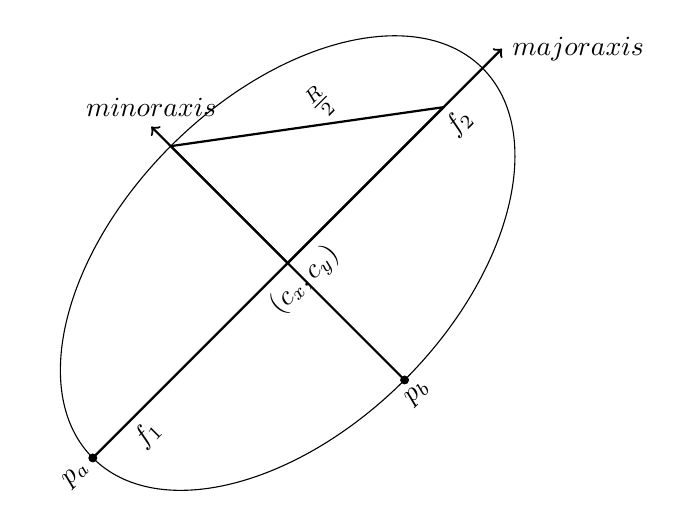
\begin{tikzpicture}[xscale=0.7, yscale=0.7][domain=0:11]
   % \draw [help axis] (-5,-3) grid (5,3);

    \begin{scope}[rotate=45]
    \draw (0,0) ellipse (5cm and 3cm);
    \node[rotate=45][below] at (-4,0) {$f_1$};
    \node[rotate=45][below] at (4,0) {$f_2$};
    \draw[fill] (-4,0) circle [radius=.5pt];
    \draw[fill] (4,0) circle [radius=.5pt];
    \draw [thick] (4,0) -- (0,0) -- (0,3) -- (4,0);
    \draw[->,thick] (-5,0)--(5.5,0) node[right]{$major axis$};
    \draw[->,thick] (0,-3)--(0,3.5) node[above]{$minor axis$};
        \node[rotate=45] [below] at (0,0) {$(c_x,c_y)$};
    \node [rotate=45][right] at (2.1,1.65) {$\frac{R}{2}$};
    
    \node [rotate=45][left] at (-5,0) {$p_a$};
    \draw[fill] (-5,0) circle [radius=2pt];
    
    \draw[fill] (0,-3) circle [radius=2pt];
    \node [below][rotate=45] at (0,-3) {$p_b$};
    \end{scope}

    %a^2-b^2=c^2 -> c^2=25-9=16 -> c=4
    
    %\draw[fill] (0,0) circle [radius=.5pt];
	
    %
    %\draw[fill] (5,0) circle [radius=1pt];
    %\draw[fill] (0,3) circle [radius=1pt];
    %
    

    %\node [below] at (2.1,0) {$c$};
	%\node [left] at (-0.1,1.5) {$b$};



    %\node [above] at (5,0) {$(x_0+a,y_0)$};
    %\node [above] at (-5,0) {$(x_0-a,y_0)$};
    %\node [above] at (0,3) {$(x_0,y_0+b)$};
    %
    

    
    %\draw [-] (-5,0) -- (5,0);
     %\draw [-] (0,-3) -- (0,3);
     %\draw [|-|] (0.001,-0.1) -- (4.999,-0.1);
\end{tikzpicture}
    \fautor
    \label{fig:ellipse_with_foci}
\end{figure}

Also, in \autoref{fig:ellipse_with_foci}, the distance $a = ||p_a - c||_2$ is called the semi-major, and the distance $b = ||p_b-c||_2$ is called the semi-minor. These two values are also referred to as the shape parameters of an ellipse. Let $d = ||c-f_1||_2$, then it is easy to see that $a = R - d$ and $b = \sqrt{\frac{R^2}{4} - d^2}$.

Finally, an ellipse is said to be axis-parallel if its major-axis (see \autoref{fig:ellipse_with_foci}), which is the line that passes through its two foci points, is parallel to the $x$-axis.

\subsection{Axis parallel}

An axis parallel ellipse centered at $c = (c_x,c_y)$ can be described using \autoref{def:ellipse} with $Q$ being a diagonal matrix \footnote{the only non-zero terms are in the main diagonal}. This can be understood as a scaling transformation applied to the euclidean norm.
Defining the matrix $Q$ as

\[
Q=
\left( {\begin{array}{cc}
    \frac{1}{a^2} & 0 \\
    0 & \frac{1}{b^2} \\
    \end{array} } \right)
\]

Then, starting from \autoref{def:ellipse}, we can obtain the following equation

\begin{align*}
        (p-c)^{T}Q(p-c) = 1\\
    (\frac{p_x-c_x}{a^2}, \frac{p_y-c_y}{b^2})^{T}(p_x-c_x, p_y-c_y) = 1
 \end{align*}
 \begin{equation}
  \frac{(p_x-c_x)^2}{a^2} + \frac{(p_y-c_y)^2}{b^2} = 1
 \end{equation}

where $a$ and $b$ are the semi-major and semi-minor shape parameters respectively.

Another way to represent ellipses, which will be useful in some occasions, is through writing it as a curve, function of the angle with its major-axis (see \autoref{fig:ellipse_params}).

\begin{figure}[H]
    \centering
    
    \caption{The ellipse as a parametric curve}
    

%\tikzset{every picture/.style={line width=0.75pt}} %set default line width to 0.75pt        

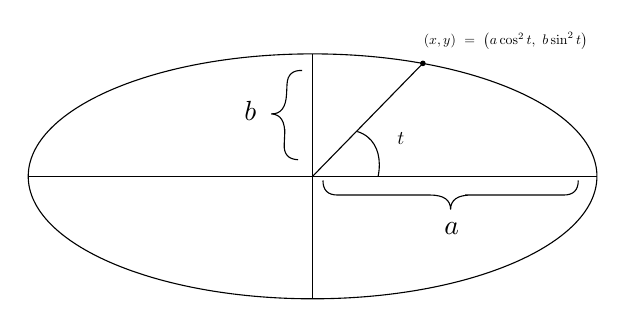
\begin{tikzpicture}[x=0.75pt,y=0.75pt,yscale=-1,xscale=1]
%uncomment if require: \path (0,300); %set diagram left start at 0, and has height of 300

%Shape: Ellipse [id:dp1559950964552308] 
\draw   (100,180) .. controls (100,147.42) and (161.34,121) .. (237,121) .. controls (312.66,121) and (374,147.42) .. (374,180) .. controls (374,212.58) and (312.66,239) .. (237,239) .. controls (161.34,239) and (100,212.58) .. (100,180) -- cycle ;
%Straight Lines [id:da3716259356733107] 
\draw    (100,180) -- (374,180) ;


%Straight Lines [id:da9880464900454329] 
\draw    (237,121) -- (237,239) ;


%Shape: Brace [id:dp3973633345998604] 
\draw   (242,182) .. controls (242,186.67) and (244.33,189) .. (249,189) -- (293.5,189) .. controls (300.17,189) and (303.5,191.33) .. (303.5,196) .. controls (303.5,191.33) and (306.83,189) .. (313.5,189)(310.5,189) -- (358,189) .. controls (362.67,189) and (365,186.67) .. (365,182) ;
%Shape: Brace [id:dp94498526835576] 
\draw   (232,129) .. controls (227.34,128.79) and (224.9,131.01) .. (224.68,135.67) -- (224.47,140.23) .. controls (224.16,146.89) and (221.68,150.11) .. (217.01,149.9) .. controls (221.68,150.11) and (223.85,153.55) .. (223.54,160.21)(223.68,157.21) -- (223.33,164.68) .. controls (223.12,169.35) and (225.34,171.79) .. (230,172) ;
%Shape: Arc [id:dp3154280429415799] 
\draw  [draw opacity=0] (258.54,158.43) .. controls (260.37,158.96) and (262.06,159.82) .. (263.54,161.03) .. controls (268.5,165.07) and (270.12,172.1) .. (268.62,179.79) -- (244.51,184.38) -- cycle ; \draw   (258.54,158.43) .. controls (260.37,158.96) and (262.06,159.82) .. (263.54,161.03) .. controls (268.5,165.07) and (270.12,172.1) .. (268.62,179.79) ;
%Shape: Circle [id:dp8908034615999807] 
\draw  [fill={rgb, 255:red, 0; green, 0; blue, 0 }  ,fill opacity=1 ] (289.08,125.57) .. controls (289.08,124.98) and (289.56,124.51) .. (290.14,124.51) .. controls (290.73,124.51) and (291.21,124.98) .. (291.21,125.57) .. controls (291.21,126.16) and (290.73,126.64) .. (290.14,126.64) .. controls (289.56,126.64) and (289.08,126.16) .. (289.08,125.57) -- cycle ;
%Straight Lines [id:da6323920079482996] 
\draw    (290.14,125.57) -- (237,180) ;



% Text Node
\draw (304,205) node   {$a$};
% Text Node
\draw (207,148.33) node   {$b$};
% Text Node
\draw (330,114.67) node [scale=0.5]  {$( x,y) \ =\ \left( a\cos^{2} t,\ b\sin^{2} t\right)$};
% Text Node
\draw (279.6,162) node [scale=0.7]  {$t$};


\end{tikzpicture}

    \fautor
    \label{fig:ellipse_params}
\end{figure}

Let $c \in \R^2$ be the center of an ellipse with shape parameters $(a,b) \in \R^2_{>0}$. Then $\gamma : [0, 2\pi] \mapsto \R^2$ defines a curve which maps every angle onto a point on the ellipse defined in \autoref{eq:parametric_ellipse}.

    \begin{equation}\label{eq:parametric_ellipse}
    \gamma(t) = \left\{
    \begin{array}{l}
    x(t)= a\cos{t} + c_x\\
    y(t)=b\sin{t} + c_y
    \end{array}
    \right.
    \end{equation}

No equivalent disk-circle wording exists for ellipses, this could be a source of ambiguity in the text, that is why a note for the reader was judged to be necessary. Throughout this work an ellipse will represent the set of points that satisfy \autoref{def:ellipse}. In some places, though, with prior clarification, we will denote as an ellipse, the set of points that are covered by the ellipse itself. For example, when we define $\Pp \cap E$ as the set of points in $\Pp$ that are covered by $E$, we are implicitly calling $E$ the set of points that are covered by the ellipse itself as it is defined by \autoref{def:ellipse}.

\chapter{Maximum Covering by Disks}
\label{chapter:pmclp}
In this chapter, we introduce a version of the classical Euclidean norm PMCLP, where each facility has a given coverage radius. 
We refer to this problem as \sigla{MCD}{Maximum Covering by Disks}. We also propose an algorithm for it to later adapt it for the elliptical PMCLP in the next chapter. 

\section{Definition}

An instance of MCD is given by a set of $n$ demand points $\Pp:=\{p_1, \dots, p_n\}$, with $p_j\in\R^2$; a set of weights $\Ww:=\{w_1, \dots, w_n\}$, with $w_j\in\R_{\ge0}$ being the weight of point $p_j$; and $m$ disks given by their radii $\Rr:=\{r_1, \dots, r_m\}$, with $r_j\in\R_{>0}$. 
Additionally, to make the text more clear, we define a set of $m$ disks as $\D:=\{D_1, \dots, D_m\}$, with $D_j : \R^2 \mapsto \R^2$ being a function that takes the center where the $j$-th disk is located as input, and returns its coverage region as defined by \autoref{eq:disk}.

A solution for an instance of MCD is determined by $Q:=(q_1, \dots, q_m) \in \R^{2m}$, which specifies the center of every disk in $\D$. Let $w: 2^{\Pp} \mapsto \R_{\ge0}$ be a function, which takes a subset of $\Pp$ and returns the sum of the weights of every point in it, defined as

\begin{equation}\label{eq:subset_w}
w(A) = \sum_{j : p_j \in A} w_j.
\end{equation}
Then an optimal solution of MCD is formulated as a solution of

\begin{equation*}
\max_{Q} w\left(\bigcup_{j=1}^m \Pp \cap D_j(q_j)\right).
\end{equation*}

It is worth mentioning that MCD is a slightly different PMCLP than the one introduced in the first study on the subject in \citeonline{church:1984}. There, a coverage radius is given for each demand, rather than for each facility, and a demand point is considered covered if a facility is located within its radius.

\subsection{CLS and CIPS}

The method proposed in \citeonline{church:1984} involves the construction of a finite set of locations where each facility can be placed as a way of transforming a problem, where every point in $\R^2$ is a possible solution, into one where only a finite number of possibilities need to be considered. This set of possible locations is called \sigla{CLS}{Candidate List Set}.

In \citeonline{church:1984}, a CLS is set to be the \sigla{CIPS}{circle intersection point set}, which contains the intersection of circles with fixed radii centered at every demand point. This approach provides an optimal solution if a complete search on the CLS for every facility is done. 

We introduce, in this chapter, a $\bigO(n^2\lg{n})$ algorithm that returns a CLS for each facility, which is based on the idea presented in \citeonline{church:1984} and in the works for the one disk case by \citeonline{chazelle:1986} and \citeonline{cabello:2006}. We refer to the CLS for the $j$-th facility as $S_j$ and prove that, indeed, an optimal solution can be found by just considering the centers in $S_j$ for each facility.

\section{Related Work}
In \citeonline{cabello:2006}, a $\bigO(n^{2m-1}\log{n})$ algorithm for $MCD$ is developed as a sub-routine for its $(1-\epsilon)$-approximation algorithm. Firstly, they solve a sub-problem for two disks in $\bigO(n^3\log{n})$. Then, for the rest of the points that are not in that solution, it uses the algorithm developed in \citeonline{chazelle:1986} for the one-disk case, checking every possible solution for every one of the disks left.

Also, in \citeonline{zhou} an heuristic method for large-scale $MCD$ is proposed. It uses a probabilistic algorithm called mean-shift which is a gradient ascent method proven to converge to a local density maxima of any probability distribution. The mean-shift is utilized to find good candidates of centers for the unit disks, then the method backtracks to find the best assignment. The results showed that the greedy algorithm achieves an optimal coverage in some instances, but for some other ones it has a 15 percent worse coverage ratio.

\section{One disk version}

This version of the problem will be refered to as \sigla{MCD1}{Maximum Covering by One Unit Disk} and it is just a specific case of MCD with only one disk with radius one ($m=1$ and $r_1=1$). We refer to an instance of MCD1 as the tuple $(\Pp, \Ww)$.
We later use the algorithm for MCD1 here described to construct a CLS which is guaranteed to contain an optimal solution for MCD.

Two exact methods for MCD1 have been found in the literature. A $\bigO(n^2)$ algorithm is proposed by \citeonline{chazelle:1986} which improved the previously $\bigO(n^2\log{n})$ one proposed by \citeonline{drezner}.
As it has been mentioned, MCD1 is a 3SUM-HARD problem, which means that it is as hard as the 3SUM problem (the problem of finding three real numbers that sum to zero, given $n$ real numbers). Initially the lower bound of the 3SUM problem was conjectured to be $\Omega(n^2)$, matching the best algorithm for MCD1, which meant that no better time-complexity could be achieved. Since then, however, better algorithms for 3SUM have been developed with a $\bigO(\frac{n^2}{poly(n)})$ run time complexity \cite{3SUM-kopelowitz:2014}.


In \citeonline{drezner}, the main idea used to develop the $\bigO(n^2\log{n})$ algorithm is that, even though there are infinitely many points where the disk could be placed, only a few of them, a finite amount of $\bigO(n^2)$, needs to be considered for the method to find an optimal solution.
The algorithm, for every point, sorts the other points with respect to the angle they form with the first one. After that, the first point is placed on the border of the disk and, going through the sorted list, the algorithm inserts and removes points from the disk coverage. Also, when inserting and removing a point from the coverage, it only checks the disk centers that make the entering/leaving point to be on the border. Because the algorithm only checks the centers that make the disk have two points on its border, the number of centers it goes through is bounded by the number of pairs of points, which is $\binom{n}{2} = \bigO(n^2)$.

The algorithm for MCD1, developed in this chapter, can be seen as a parallel version of the algorithm developed by \citeonline{drezner}.
We, however, based on \citeonline{chazelle:1986} and \citeonline{cabello:2006}, decided to work with an equivalent problem called \sigla{MWC}{Maximum Weight Clique} which is introduced in the next section.

\section{Maximum Weight Clique}

An instance of the \sigla{MWC}{Maximum Weight Clique} is given by a list of points \mbox{$\Pp:=\{p_1,\dots,p_n\}$}, with $p_i \in \R^2$ representing the center of a unit disk;  and \mbox{$\Ww:=\{w_1, \dots, w_n\}$}, with $w_i\in \R_{>0}$ being the weight of the $i$-th unit disk. We also define a list $\D=\{D_1, \dots, D_n\}$, such that $D_i$, $i\in\{1,\dots,n\}$, is a unit disk centered at $p_i$ having weight $w_i$ assigned to it.

A clique, in this context, is a non-empty intersection region of one or more disks, and its weight is the sum of the weights of those disks in the intersection.
Following this, a solution for MWC can be defined as just a point $q\in\cup_{j=1}^n D_j$, which is inside any of the given disks in $\D$.
From a solution $q$, the corresponding clique $S$ can be obtained by intersecting every disk that contains $q$ as follows

\begin{equation*}
S = \bigcap_{j : q \in D_j} D_j.
\end{equation*}

With a geometric observation, though, the number of possible values for the solution can be reduced.
Let $\partial \D = \{ \partial D_1, \dots, \partial D_n \}$ be the set of circles corresponding to each disk in $\D$. 
Unless a clique is formed by only one disk, its boundary contains at least two points, which are the intersection of two circles that are part of the clique.
Because of that, $q$ can be limited to the set of pairwise intersections of $\partial \D$ as well as the set of centers of each disk $\Pp$, which considers the case where the optimal clique is composed of only one disk. With this observation, an optimal solution of MWC can be defined by the optimization problem

\begin{equation*}
\max_{q} \sum_{D_k \cap q \neq \emptyset} w_k,
\end{equation*}
with $q \in \{\partial D_i \cap \partial D_j : 1 \le i < j \le n\} \cup \Pp$. With this new specification of the solution's search space, given an instance of MWC, an optimal solution can be found by going through $\binom{n}{2} + n$ points, that is, $\bigO(n^2)$ points.

It is worth pointing out that MWC is a different problem than the maximum clique on a intersection graph (a graph where the vertices are the disks and an edge exists if there is an intersection between two disks). 
As shown in \autoref{fig:three_disks_no_intersection}, three disks could have non-empty pairwise intersection and still have an empty intersection of all of them together.
That is why MWC is also referred to as the Maximum Geometric Clique Problem and the other version, when there is only the pairwise intersection condition, is referred to as the Maximum Graphical Clique Problem \cite{inplace:2014}. 

%The graphical version of the problem was studied by \citeonline{graphical-clique}, where a $\bigO(n^{4.5})$ algorithm was proposed. Also, in \citeonline{inplace:2014}, a $\bigO(n^2\log{n})$ time in-place algorithm\footnote{An in-place algorithm is an algorithm that needs $\bigO(1)$ extra space.} for arbitrary radii disks was proposed. 

In \citeonline{chazelle:1986}, the method for MWC consists on building a planar graph on which the vertices are the $\binom{n}{2}$ pairwise intersection of the circumferences and the edges are the arcs of the circumferences connecting the intersections. With the graph constructed, a traversal is done to obtain the answer, thus the time complexity of $\bigO(n^2)$.

As it has been mentioned, with the equivalence of the two problems, an optimal solution of the Maximum Weight Clique Problem is also an optimal solution of MCD1, which means that a disk centered at $q^*$ which is an optimal solution of MWC, will have a maximal weight covering of the demand set $\Pp$.

Given an instance of MCD1, the equivalent MWC intance is obtained by defining the set $\D$ to contain the disks centered at $\Pp$ and setting the weight of every disk to be the weight of its corresponding point in $\Pp$. A disk $D_i$ will represent the area where a disk can be placed in order to cover $p_i$. This means that an intersection between some disks is a region where a disk could be placed to cover the corresponding points.

In \autoref{fig:three_disks_no_intersection}, it can be seen that there is no point where a disk could be placed such that it would cover $p_1, p_2$ and $p_3$, nonetheless, in any of the pairwise intersections, a disk could be placed to cover the two corresponding points.

\begin{figure}[h]
	\centering
	
	\caption{Three disks that have non-empty pairwise intersection among them, but no common intersection.}
	
	\includegraphics[scale=.25]{tex/figures/three_disks_no_intersection.pdf}
	\label{fig:three_disks_no_intersection}
	\fautor
\end{figure}

Formally, in MWC, if a point $q$ lies inside $\bigcap_{k \in I} D_k$, with $I \subset \{1,\dots,n\}$, then a disk centered at $q$ will cover the points $p_k$, with $k\in I$ in the equivalent MCD1 instance. Conversely, the same applies for a disk placed at $q$ that covers points $p_k$, with $k \in I$ in the MCD1 instance. It means that $q$ will lie inside region $\bigcap_{k \in I} D_k$ in MWC.

\subsection{An algorithm for the Maximum Weight Clique Problem}

The algorithm described here is based on the one in \citeonline{drezner}, also with some ideas from \citeonline{inplace:2014} and \citeonline{cabello:2006}. It has a run time complexity of $\bigO(n^2\log{n})$ and uses $\bigO(n)$ of extra space. It is worth noting, though, that a $\bigO((n+K)\log{n})$ run time, with $K$ being the number of intersections, can be obtained by using the algorithm in \citeonline{bentley:1979} to find all the intersections among the $n$ circumferences.

In \citeonline{inplace:2014} an important observation is made about the intersection regions of disks. Given an instance of MWC, any clique formed by a subset of $\D$ is bounded by the arcs of circles that intersect with it. Also, those arcs have the intersection of circles as their end-points. This can be seen on \autoref{fig:3disks_intersect} where the cliques that $D_1$ is part of are bounded by $D_1$'s arcs which have its intersections with the other circles as end-points. Following this, a definition is presented to characterize the end-points of an arc bordering a clique.

\begin{definicao}\label{def:inter_arc}
    Let $D_i$ and $D_j$ be two unit disks with non-empty intersection, and \mbox{$(\theta_1, \theta_2) \in [0,2\pi)^2$} be the two angles that $\partial D_i$ and $\partial D_j$ intersect, with the condition that $(\theta_1,\theta_2)$ defines an arc (counter-clockwise order) of $D_i$ that is the border of $D_i \cap D_j$. Then, define $\Gamma_+(i,j) = \theta_1$ and $\Gamma_-(i,j) = \theta_2$. For convenience, if $D_i$ is tangent to $D_j$, then $\theta_1=\theta_2$; and if $i=j$, then $\Gamma_+(i, j)=0$ and $\Gamma_-(i,j)=2\pi$.
\end{definicao}

\begin{figure}
\centering

    \caption{Three disks and their intersection points.}
    \includegraphics[scale=.3]{tex/figures/3_disks_intersect.pdf}
%    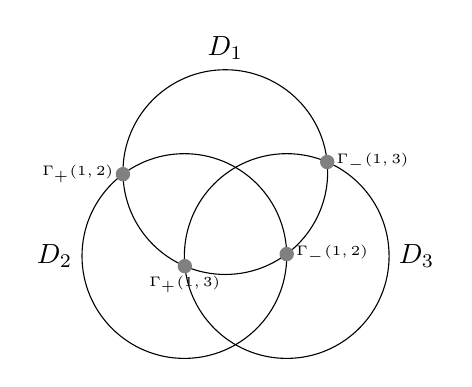
\begin{tikzpicture}[scale=1.3]
%\draw [help lines] (-5,-3) grid (5,3);

\draw[name path = c1] (0,0) circle (1cm);
\draw[name path = c3] (0.6,-0.82) circle (1cm);
\draw[name path = c2] (-0.4,-0.82) circle (1cm);

\node[above] at (0, 1) {$D_1$};
\node[left] at (-1.4, -0.82) {$D_2$};
\node[right] at (1.6, -0.82) {$D_3$};

\path [name intersections={of=c1 and c3}] ;
\foreach \i in {1,...,2}
\fill [color=gray] (intersection-\i) circle (2pt) ;

\node[right] at (intersection-1) {\tiny $\Gamma_-(1,3)$};
\node[left, below] at (intersection-2) {\tiny $\Gamma_+(1,3)$};

\path [name intersections={of=c1 and c2}] ;
\foreach \i in {1,...,2}
\fill [color=gray] (intersection-\i) circle (2pt) ;

\node[left] at (intersection-1) {\tiny $\Gamma_+(1,2)$};
\node[below,right] at (intersection-2) {\tiny $\Gamma_-(1,2)$};

%\draw [-] (-5,0) -- (5,0);
%\draw [-] (0,-3) -- (0,3);
%\draw [|-|] (0.001,-0.1) -- (4.999,-0.1);
\end{tikzpicture}
    \fautor
    \label{fig:3disks_intersect}
\end{figure}

Also, we refer to $\Gamma_+(i,j)$ as an opening angle, and to $\Gamma_-(i,j)$ as a closing angle. In \autoref{fig:3disks_intersect}, it is shown all the intersection points between $D_1$ with $D_2$ and $D_3$. Also, they are labeled according to \autoref{def:inter_arc}. Note that $\Gamma_+(1,3) > \Gamma_-(1,3)$ (the angles should be in the $[0,2\pi]$ interval).

With \autoref{def:inter_arc} in hand, we can establish the basis of the algorithm for MWC. For every disk $D_i$, let us describe an algorithm that gets the best clique which $D_i$ is part of. This way, an algorithm for MWC just uses that method for every disk and returns the best solution found. Firstly, let $A_i$ be a circular list that contains the intersection angles of $\partial D_i$ with every circle in $\partial \D$ defined as
\begin{equation*}
A_i = \bigcup_{j=1}^n \{ \Gamma_-(i,j), \Gamma_+(i,j) \}.
\end{equation*}
Assume also that $A_i$ is sorted in ascending order by the angle values with ties being broken by prioritizing opening angles.

Finding the best solution which $D_i$ is part of can be done by traversing $A_i$ while keeping a set of active disks. When an opening intersection angle is reached, the corresponding disk is added to the active set; and when a closing one is seen, the corresponding disk is removed from the active set. This way, finding an optimal solution can be achieved by keeping the weight of the active disks as well as the best clique found so far. Notice also that because $\Gamma_+(i,i)=0$ and $\Gamma_-(i,i)=2\pi$, any clique found by the traversal will also contain $D_i$.

In practice, traversing a circular list can be emulated by traversing a regular list that has a copy of the original circular list added to its end. 
Therefore, the list $B_i$ is defined here as a list that contains the elements of $A_i$ and a copy of it shifted to the interval $[2\pi, 4\pi]$. It is defined as

\begin{equation}\label{eq:b_i}
B_i = A_i\cup\bigcup_{j=1}^n \{ 2\pi+\Gamma_-(i,j), 2\pi+\Gamma_+(i,j) \}.
\end{equation}
Assuming $B_i$ is sorted with the same criteria as $A_i$, a simple traversal, starting at the first element and going until the last one, simulates a traversal on the circular list $A_i$.
This works because for any pair of disks $D_i$, $D_j$; $B_i$ contains $\Gamma_+(i,j) < \Gamma_-(i,j) + 2\pi$. That is, the algorithm encounters an opening angle before reaching a closing one for any circle.

In \autoref{fig:array_disks}, the intersection points between $\partial D_1$ (solid border) with $\partial D_2, \partial D_3$, and $\partial D_4$ (dashed border) are shown with a plus or minus sign indicating opening or closing intersection angles. 
The intersection list $B_1$ is also displayed in \autoref{fig:array_disks} along with the size of the set of active disks $Q$ after processing a point in $B_1$ -- this is exactly what \autoref{algoritmo:mcd_1} for MWC does for every disk. 
It is possible to see that the optimal clique highlighted in \autoref{fig:array_disks} is enclosed by the arcs defined by $\Gamma_+(1,4)$ and $\Gamma_-(1,4)$, and can also be identified by following $B_1$ while keeping track of $Q$.
The special intersection point of $\partial D_1$ with itself can also be seen in \autoref{fig:array_disks}. Its usage is very convenient as with $\Gamma_+(1, 1)$ and $\Gamma_-(1,1)$  in $B_1$, the algorithm inserts $D_1$ in the set of active disks before processing any point, and removes $D_1$ only after every point has been processed.
\begin{figure}[H]
	\centering
	
	\caption{The intersection list of a disk with three other disks.}
	%\input{tex/figures/array_disks.tex}
	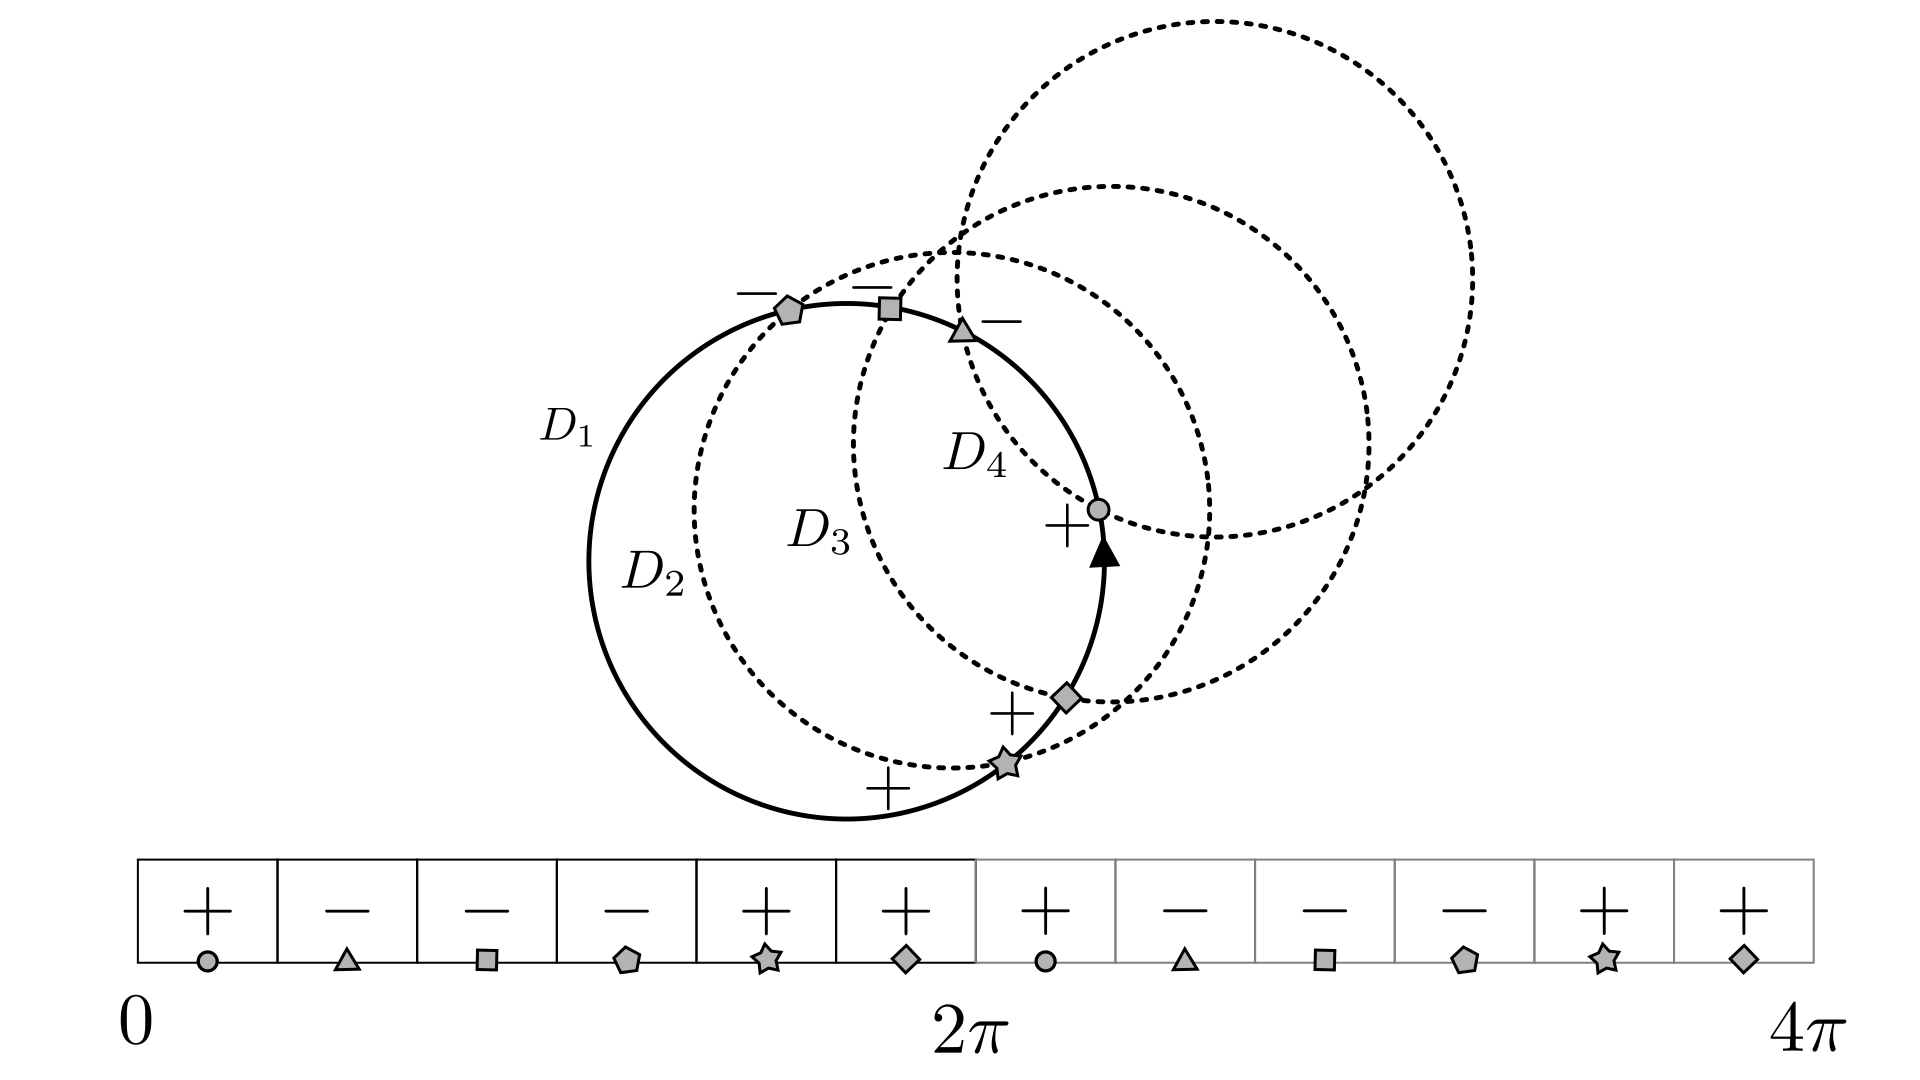
\includegraphics[scale=.3]{tex/figures/3_disks_intersect2.pdf}
	\fautor
	\label{fig:array_disks}
\end{figure}

Finally, we define \autoref{algoritmo:mcd_1} for MWC. Given an instance $(\Pp, \Ww)$ of MWC, the algorithm uses the approach described here of keeping a set of active disks while traversing the list $B_i$. It returns a point that is inside an optimal clique, this way \autoref{algoritmo:mcd_1} can also be used to get an optimal solution for an instance $(\Pp, \Ww)$ of MCD1.
\clearpage
\begin{algoritmo}[!htb]
	\caption{Algorithm for MWC.}\label{algoritmo:mcd_1}
	\begin{algorithmic}[1]
		\Require{A set of points $\Pp=\{p_1,\dots,p_n\}$, and a set of weights $\Ww=\{w_1, \dots, w_n\}$.}
		\Ensure{A point that is inside the maximum weight clique of unit disks.}
		
		\item[]
		
		\Procedure{$MWC$}{$\Pp, \Ww$}
		\State Let $\D=\{D_1, \dots, D_n\}$ be a set of unit disks, with centers in $\Pp$ and weights in $\Ww$
		
		\State $Q_{best} \gets \{\}$
		\State $q^* \gets$ $p_1$
		\ForAll{$D_i \in \D$}
		\State Let $B_i$ be the list of intersection angles of $D_i$ as defined by \autoref{eq:b_i}
		
		\State $Q \gets \{\}$ \Comment{The set of active disks.}
		\For{$\theta \in B_i$}\Comment{Assuming $B_i$ is sorted.}
		\State Let $D_j$ be the disk, such that $\theta \in D_j\cap D_i$
		\If{$\theta$ is a opening angle}
		\State $Q \gets Q \cup \{D_j\}$
		\Else
		\State $Q \gets Q \setminus \{D_j\}$
		\EndIf
		\If{$w(Q_{best}) < w(Q)$} 
		\State $Q_{best} \gets Q$
		\State $q^* \gets$ point corresponding to the intersection angle $\theta$
		\EndIf
		
		\EndFor
		\EndFor
		
		\State \Return $q^*$
		\EndProcedure
	\end{algorithmic}
\end{algoritmo}

\begin{theorem}\label{lema:disk}
	\autoref{algoritmo:mcd_1} for solving the Maximum Clique Problem has a $\bigO((n+K)\log{n})$ run time complexity, where $K$ is the number of intersections of the $n$ disks.
\end{theorem}

\begin{proof}
	Finding every intersection can be done in $\bigO((n+K)\log{n})$  by a plane sweep, the method is described in \citeonline{bentley:1979}. 
	Because sorting the intersection angles needs to be done, an additional $\bigO(K\log{K})$ pre-processing is added. All the other operations can be done in constant time. Therefore, the final algorithm complexity is $\bigO((n+K)\log{n})$.
\end{proof}

If a simpler implementation is desired, or the number of intersections is large, determining the set $I_i$ (the set of disks that intersect with $D_i$, defined in \autoref{algoritmo:mcd_1}) can be simply done in $\bigO(n^2)$, making the algorithm have a worst-case complexity of $\bigO(n^2\log{n})$.


\section{An algorithm for MCD}

A simple adaptation can be done on \autoref{algoritmo:mcd_1} to make it return a CLS that contains an optimal solution of MCD for that disk. This is shown in \autoref{algoritmo:mcd_cls}. 
Notice also that MCD1 is defined only for unit disks, however, this constraint can be dropped, as it is introduced just for the sake of keeping the text more simple and \autoref{algoritmo:mcd_1} works for any radius. A result about the runtime complexity of \autoref{algoritmo:mcd_cls} has already been given by \autoref{lema:disk}, the following result states about the adaption of it to be used in an algorithm for MCD.

\begin{lema}\label{lema:mcd}
	Suppose that an instance of MCD and an index $j\in\{1, \dots, m\}$ are given.
	Then \autoref{algoritmo:mcd_cls}, when given the instance $(\Pp, \Ww, r_j)$ as input, returns a CLS $S_j$ of size $\bigO(n^2)$, such that $q^*_j\in S_j$, with $(q^*_1, \dots, q^*_m)$ being an optimal solution of the given MCD's instance.
\end{lema}

\begin{proof}
It can be seen that in any solution of MCD, a disk placed at a point $q$ that covers at least one point $p \in \Pp$ has a correspondence to the Maximum Weight Clique Problem: the point $q$ is inside an intersection area of at least one disk and that area is bounded by some disk, which means it will be checked by \autoref{algoritmo:mcd_cls} as a candidate to be an optimal solution. The number of points \autoref{algoritmo:mcd_cls} goes through is $\bigO(n^2)$, then
obviously $|S_j|=\bigO(n^2)$.
\end{proof}

Then, with \autoref{algoritmo:mcd_cls}, an algorithm for MCD that checks every possible center for every disk yields a $\bigO(n^{2m})$ run-time complexity.
This algorithm is described in \autoref{chapter:ellipses} for the axis-parallel ellipses case.

It is worth mentioning that the choice of developing a different method for the problem, instead of using the one from \citeonline{cabello:2006}, is taken for the sake of simplicity, considering both algorithms achieve similar bounds.

\begin{algoritmo}
	\caption{Algorithm for MCD1 that returns a CLS.}\label{algoritmo:mcd_cls}
	\begin{algorithmic}[1]
		\Require{A set of points $\Pp=\{p_1,\dots,p_n\}$ with weights $\Ww=\{w_1, \dots, w_n\}$, and a radius $r\in\R_{>0}$.}
		\Ensure{A CLS for the disk given by radius $r$.}
		
		\item[]
		
		\Procedure{CLS-MCD}{$\Pp, \Ww, r$}
		\State $S \gets \{\}$
		\ForAll{$p_i \in \Pp$}
		%\State Let $D_i(p_i)$ be the disk with center at $p_i$
		\State Let $B_i$ be the list of intersection angles of $\partial D_i(p_i)$ as defined by \autoref{eq:b_i}
		
		\For{$\theta \in B_i$}\Comment{Assuming $B_i$ is sorted.}
		\If{$\theta$ is a opening angle}
		\State Let $q_\theta$ be the intersection point correspondent to angle $\theta$
		\State $S \gets S \cup \{q_\theta\}$	
		\EndIf
		\EndFor
		\EndFor
		
		\State \Return $S$
		\EndProcedure
	\end{algorithmic}
\end{algoritmo}

\chapter{Maximum Covering by Ellipses}
\label{chapter:mce}
In this chapter, we introduce the version of PMCLP where every 
facility has an axis-parallel ellipse as its coverage area. We refer to this problem as \sigla{MCE}{Maximum Covering by Ellipses}. We also present an algorithm for it which is an adaptation of the algorithm developed for MCD in \autoref{chapter:pmclp}.

\section{Definition}

Axis-parallel ellipses are defined as the set of points that satisfy \autoref{equation:pellipse}. Note that all it takes to describe an axis-parallel ellipse is a pair of positive real numbers $(a,b) \in \R_{>0}^2$, also called its shape parameters, and a center point $q \in \R^2$.

An instance of MCE is given by a set of $n$ demand points $\Pp = \{p_1, \dots, p_n\}$, with $p_j\in\R^2$; 
a set of weights $\Ww:=\{w_1, \dots, w_n\}$, with $w_j\in\R_{\ge0}$ being the weight of point $p_j$;
and a set of $m$ axis-parallel ellipses given by their shape parameters $\Rr:=\{(a_1, b_1), \dots, (a_m, b_m)\}$, with $(a_j, b_j)\in\R_{>0}^2$ and $a_j>b_j$.
Additionally, to make the text more clear, we define a set $\E = \{E_1, \dots, E_m\}$, with $E_j : \R^2 \mapsto \R^2$ being a function that takes the center where the $j$-th ellipse is located as input, and returns its coverage region as defined by \autoref{equation:cover_pellipse}.

Then, a solution for MCE is given by $Q:=(q_1, \dots, q_m)\in\R^{2m}$, with $q_j$ being the center of $j$-th ellipse. Finally, let $w : 2^\Pp \mapsto \R_{\ge0}$ as defined by \autoref{eq:subset_w}, then an optimal solution of MCE is given by the optimization problem

\begin{equation*}
\max_q w\left(\bigcup_{j=1}^m \Pp \cap E_j(q_j)\right).
\end{equation*}

In the next sections, we first describe a method for the case with only one ellipse, and then use it in the algorithm for multiple ellipses to construct a CLS containing an optimal solution.

\section{Related work}
The maximal planar covering using axis-parallel ellipses was first introduced in \citeonline{canbolat} which proposed a mixed integer non-linear programming method for the problem. This first approach showed to be not that efficient as it could not find an optimal solution for some instances within a timeout defined by them. To obtain solutions, not necessarily optimal ones, for the instances which the exact method showed inefficiency, a heuristic technique called Simulated Annealing was used to develop another method. Comparisons were made, which showed that the second approach was able to obtain good solutions, compared to the optimal ones found for some of the instances, within a good run-time.

The second work found in the literature was \citeonline{andreta}, which developed a method that breaks the problem into smaller ones fixing the set of points an ellipse is going to cover. For each set of points fixed as the points an ellipse is going to cover, a small optimization problem is solved to find out if there is a location where the ellipse can be placed, so to cover the set of fixed points. To enumerate the possible solutions and then find an optimal one, the method defined a data structure that stores every set of points an ellipse can cover. This method showed better results and was able to find optimal solutions for the instances that the first method could not get as well as for new created instances.

\section{One Ellipse Version}

The case with only one ellipse is considered first because it will be adapted to become the basis of the algorithm for more than one ellipse. We refer to this version as \sigla{MCE-1}{Maximum Cover by One Ellipse}. 

An instance of MCE-1 has $m=1$, and we set $(a, b):=(a_1, b_1)$, and $\E := \{E\}$. Therefore, an instance of MCE-1 is described by the tuple $(\Pp; \Ww; (a, b))$. A solution of MCE-1 is then given by a point $q\in\R^2$, and an optimal solution is given by the optimization problem

\begin{equation*}
\max_q w(\Pp \cap E(q)).
\end{equation*}
An adaptation of \autoref{algoritmo:mcd_1} is obtained by just replacing the function that finds the intersection points between two disks by a function that finds the intersection points between two ellipses $\partial E_i$ and $\partial E_j$.
It can be seen in \autoref{fig:3ellipses_intersect} that the intersection points and their correspondents $\Gamma_-(i,j)$ and $\Gamma_+(i,j)$ functions behave the same way as in the disks case.
The intersection of two ellipses as well as determining $\Gamma_-(i,j)$ and $\Gamma_+(i,j)$ are described in the next section.

\begin{figure}[H]
	\centering
	\caption{Three ellipses and their intersection points}
	\includegraphics[scale=.34]{tex/figures/3ellipses_intersect.pdf}
	\fautor
	\label{fig:3ellipses_intersect}
\end{figure}

\section{Determining $\Gamma_+(i,j)$ and $\Gamma_-(i,j)$}\label{section:ellipses_intersection}

Let $E_1(q_1)$, and $E_2(q_2)$ be two coverage region of ellipses centered at $q_1, q_2\in\R^2$ respectively, with shape parameters $(a, b)\in\R^2_{>0}$. After changing the coordinates to make the center of the first ellipse be at the origin, the intersection points between the two ellipses are defined by

\begin{align}
\frac{x^2}{a^2} + \frac{y^2}{b^2} = 1 && (E_1) \label{eq:ell_inter_1}\\
\frac{(x-h)^2}{a^2} + \frac{(y-k)^2}{b^2} = 1 && (E_2), \nonumber
\end{align}
where $(h,k)\in\R^2$ is the center of the second ellipse after the coordinates were translated by $-q_1$. As both equations are equal to $1$, we have
\begin{align}
    b^2x^2 + a^2y^2 &= b^2(x-h)^2 + a^2(y-k)^2 \nonumber\\
    x &= y\frac{-2ka^2}{2hb^2} + \frac{b^2h^2 + a^2k^2}{2hb^2} \nonumber\\
    x &= y\alpha + \beta.\label{eq:ell_inter_2}
\end{align}
Replacing \autoref{eq:ell_inter_2} into \autoref{eq:ell_inter_1}, we get
\begin{align}\label{eq:ell_inter_3}
y^2(b^2\alpha^2 + a^2) + y(2\beta\alpha b^2) + b^2\beta^2 -a^2b^2 = 0,
\end{align}
Which is a second degree polynomial. Then, $\partial E_1(q_1) \cap \partial E_2(q_2) \neq \{\}$ if, and only if the roots of \autoref{eq:ell_inter_3} are real. The intersection points itself can be obtained by solving the polynomial for $y$ and applying its value onto the $x=y\alpha + \beta$ equation.

Suppose that $\partial E_1(q_1) \cap \partial E_2(q_2) = \{p_1, p_2\}$, with $p_1 \neq p_2$. To determine $\Gamma_+(1,2)$ and $\Gamma_-(1,2)$, we need to first determine the angles of intersection of $p_1$ and $p_2$ on $E_1(q_1)$ using the parametric equation for an ellipse defined in \autoref{eq:parametric_ellipse}. Given a point $(x, y)\in \partial E_1(q_1)$, using \autoref{eq:parametric_ellipse} we have

\begin{equation*}
\dfrac{a}{b}\dfrac{y-q_{1y}}{x-q_{1x}} = \tan{t}.
\end{equation*}
Solving for $t$ gives the angle of point $(x,y)$ on $E_1(q_1)$. Using that process we obtain $t^{(1)}_1, t^{(1)}_2$ as the angles of the points $\{p_1, p_2\}$ on $E_1(q_1)$; and $t^{(2)}_1, t^{(2)}_2$ as the angles of points $\{p_1, p_2\}$ on $E_2(q_2)$.
Let $\gamma_1$ be the curve defined by $E_1(q_1)$ and $\gamma_2$ the curve defined by $E_2(q_2)$. Considering its derivatives \autoref{eq:der_parametric_ellipse} at the intersection points, as it can be seen in \autoref{fig:ellipse_gamma}, we have that $p_1$ is $\Gamma_+(1,2)$ if, and only if
\begin{equation*}
angle(\gamma_1'(t_1^{(1)}), -\gamma_2'(t_1^{(2)}) < \pi.
\end{equation*}
The case where that angle is equal to $\pi$ happens when both ellipses intersect at only one point. This case has to be treated separately as we need to have two equal intersection points: one as $\Gamma_+(1,2)$ and the other as $\Gamma_-(1,2)$.

\begin{figure}
	\centering
	
	\caption{The intersection list of a disk with three other disks.}
	%\input{tex/figures/array_disks.tex}
	\includegraphics[scale=.38]{tex/figures/ellipse_gamma.pdf}
	\fautor
	\label{fig:ellipse_gamma}
\end{figure}

\section{An algorithm for MCE}

The same procedure defined in \autoref{algoritmo:mcd_cls} can be used to get a CLS for every ellipse in MCE. We refer to the elliptical version of that procedure as CLS-MCE (we do not define it in this chapter because it would look the same as CLS-MCD defined in \autoref{algoritmo:mcd_cls}, apart from the name, of course). 

Then, with the algorithm to construct a CLS for every ellipse in hands, an algorithm for MCE naturally comes into existence. In \autoref{algoritmo:mce}, a complete search is done backtracking every possibility in the CLS of every ellipse. This strategy is backed-up by \autoref{lema:mcd}, which says that there is an optimal solution in the CLS of each ellipse. 
Following this, counting every possibility that the algorithm goes through, we arrive at the run-time complexity of $\bigO(n^{2m})$.

It is worth mentioning that, even though we call CLS-MCE every time in the recursion, in practice, it is probably best to pre-process this step, and only call it $m$ times for the whole set of points.
Some other easy improvements can also be made in the implementation. For example, if an ellipse covers two sets of points $X$ and $Y$, with $X \subset Y$, then set $X$ can be ignored by the algorithm because of the non-negative weights constraint. Also, if two ellipses have their centers with Euclidean distance greater than their semi-major parameter, they for sure do not intersect. Depending on the input, this observation can make the algorithm not go through the whole list of ellipses every time it needs to determine the ellipses pairwise intersections.

\section{Adding facility cost}

Additionally, in \citeonline{andreta} and \citeonline{canbolat}, two other parameters are present in the definition of the problem. This extension is the result of having costs associated with every facility.
In MCE, though, the total cost, which is the sum of costs of every used facility, is constant; hence, to create a decision about which ones are utilized, a new parameter $k\in\mathbb{N}$ is given, along with a constraint on the number of used ellipses.

We refer to this version of the problem as  \sigla{MCE-$k$}{Maximum Covering by Ellipses with a $k$-constraint}. An instance of it is given by the same parameters as MCE, plus a list of costs $\Cc=\{c_1, \dots, c_m\}$, with $c_j\in\R_{\ge0}$ being the $j$-th ellipse's cost, and $k\in\mathbb{N}$, $k\le m$.

 A solution for MCE-$k$, however,  when compared to MCE's, has a bit more cluttered description. We define it as a set $I:=\{i_1, \dots, i_k\}\subset\{1, \dots, m\}$, such that $|I|=k$; and a tuple $Q:=(q_1, \dots, q_k)$, with $q_j\in\R^2$ being the center of the $j$-th ellipse in $I$. An optimal solution of MCE-$k$ is given by the optimization problem

\begin{equation*}
\max_{I, Q} w\left(\bigcup_{j=1}^k \Pp \cap E_{i_j}(q_j)\right).
\end{equation*}

Finally, \autoref{algoritmo:mce} can serve as basis for the \autoref{algoritmo:mce-k} for MCE-$k$. 
Firstly, for every subset $I \subset \{1, \dots, m\}$, such that $|I| = k$, the algorithm for MCE is invoked for the instance $(\Pp, \Ww, \{(a_j, b_j) : j \in I\})$; that is, an instance where only the ellipses in $I$ are present.
After that, by keeping track of the utilized ellipses' costs for every $I \subset \{1, \dots, m\}$, an optimal solution can be obtained.
This simple adjustment achieves a run-time complexity of $\bigO(\binom{m}{k} \times n^{2k}) = \bigO(n^{3m})$. 

\begin{algoritmo}
    \caption{Algorithm for MCE}\label{algoritmo:mce}
    
    \begin{algorithmic}[1]
        \Require{A set of points $\Pp=\{p_1,\dots,p_n\}$, a list of weights $\Ww=\{w_1, \dots, w_n\}$, and a list of shape parameters $\Rr=\{(a_1, b_1), \dots, (a_m, b_m)\}$.}
        
        \Ensure{An optimal solution for MCE.}
        
        \item[]
        \Procedure{$MCE$}{$\Pp, \Ww, \Rr$}
	    \State \Return $MCE_{bt}(\Pp, \Ww, \Rr, 1)$
        \EndProcedure
        
        \Procedure{$MCE_{bt}$}{$Z, \Ww, \Rr, j=1$}
        \If{$j = m+1$}
        \State \Return $0$
        \EndIf
        
        \State $(q_j^*, \dots, q_m^*) \gets (0, \dots, 0)$

        \State $S_j \gets \textnormal{CLS-MCE}(Z, a_j, b_j)$
        \For{$q_j \in S_j$}
        \State $Cov \gets \Pp \cap E_j(q_j)$
        \State $(q_{j+1}, \dots, q_m) \gets MCE_{bt}(Z \setminus Cov, \Ww, \Rr, j+1)\}$
        
        \If{$w(Cov) + w(\cup_{k=j+1}^m Z \cap E_k(q_k)) >  w(\cup_{k=j}^m Z \cap E_k(q_k^*))$}
        \State $(q_j^*, \dots, q_j^*) \gets(q_j, \dots, q_m)$
        \EndIf
        \EndFor

        \State \Return $(q_j^*, \dots, q_m^*)$
        \EndProcedure
    \end{algorithmic}
\end{algoritmo}

\begin{algoritmo}
	\caption{Algorithm for MCE-$k$}\label{algoritmo:mce-k}

	
	\begin{algorithmic}[1]
   \Require{A set of points $\Pp=\{p_1,\dots,p_n\}$, a list of weights $\Ww=\{w_1, \dots, w_n\}$, a list of shape parameters $\Rr=\{(a_1, b_1), \dots, (a_m, b_m)\}$, a list of costs $\Cc=\{c_1, \dots, c_m\}$, and $k\in \mathbb{N}$.}
	\Ensure{An optimal solution for MCE-$k$.}
	        
	\item[]
	
\Procedure{MCE-$k$}{$\Pp, \Ww, \Rr, \Cc, k$}
	\State $I^* = \{i_1^*, \dots, i_k^*\}\gets \{1, \dots, k\}$
	\State $Q^* = (q_1^*, \dots, q_k^*) \gets (0, \dots, 0)$
	
	\ForAll{$I=\{i_1, \dots, i_k\} \subset \{1, \dots, m\}$, such that $|I|=k$}

		\State $(q_1, \dots, q_k) \gets MCE(\Pp, \Ww, \{(a_j, b_j) \in \Rr: j \in I\})$
		
			
		\If{$w(\bigcup_{j=1}^k \Pp \cap E_{i_j}(q_j)) - \sum_{j\in I} c_j > w(\bigcup_{j=1}^k \Pp \cap E_{i_j^*}(q_j^*)) - \sum_{j\in I^*}c_{j}$}
			\State $Q^* \gets (q_1, \dots, q_k)$
			\State $I^* \gets I$
		\EndIf
	\EndFor
	
	\State \Return $I^*, Q^*$
\EndProcedure
	\end{algorithmic}
\end{algoritmo}

%\chapter{Every Center and Angle of Rotation of an ellipse given its shape and three points}
\chapter{Determining every location of an ellipse given its shape and three points}
\label{chapter:e3p}
The problem of finding every center and angle of rotation of a fixed shape ellipse which makes it have three points on its border is presented in this section. Even though its simple statement--it is short and uses only basic mathematical concepts--we were not able to find any work on it, or even on related problems. 
As a result, starting from scratch, we ended up trying a handful of approaches with most of them failing on the way. We try to give a review of some of those, and also make a case for the method we propose in terms of velocity of convergence and quality of the solutions that it finds.

We refer to this problem as \sigla{E3PNT}{Ellipse by Three points}, and an instance of it is given by three points $u, v, w \in \R^2$ and $E$, an ellipse with shape parameters $(a, b) \in \R^2_{>0}$, with $a > b$. A solution of E3PNT is a pair $(q, \theta) \in \R^2\times[0, \pi]$, such that $\{u, v, w\} \subset \tilde{E}(q, \theta)$. In other words, the goal is to develop a method to find every solution of E3PNT. 


\section{Transforming the problem}

To make it simpler, let us translate the system, so the point $u$ is at $(0,0)$. Then, we assume that the ellipse is actually axis-parallel and the points are the ones rotating. When an angle is found such that the three points lie on the border of the axis-parallel ellipse, a linear transformation can be applied to compress the x-axis by $\frac{b}{a}$, transforming the ellipse into a circle of radius $b$. This transformation can be seen on \autoref{fig:circumscribed-circle} where a solution of the E3PNT is transformed into a solution of the problem of finding a circumscribed circle of a triangle. 
This process can be parametrized by the angle of rotation of the points, as described by \autoref{eq:trpnts}, and because of the invertibility of linear transformations solutions for E3PNT can be obtained by reversing the transformations.

\begin{figure}
	\centering
	\caption{Transforming an ellipse into a circle. T1, T2, and T3 represent the steps of the transformation.}
	\includegraphics{tex/figures/scripts/circumscribed-circle}
	\fautor
	\label{fig:circumscribed-circle}
\end{figure}
\begin{equation}\label{eq:trpnts}
\varphi(p, \theta)=\left[\begin{array}{cc}
\frac{b}{a}&0\\
0&1
\end{array}\right]
\left[\begin{array}{cc}
\cos{\theta}&\sin{\theta}\\
-\sin{\theta}&\cos{\theta}
\end{array}\right]\left[\begin{array}{c}
p_x\\
p_y
\end{array}\right].
\end{equation}

Then, the problem to be solved is finding a circumscribed circle of the triangle formed by the points $(0, 0), \varphi(v, \theta)$ and $\varphi(w, \theta)$, such that the circle has radius $b$. As, for three non-colinear fixed points, there is always an unique circumscribed circle for the triangle formed by those three points, the only variable to be determined ends up being the angle of rotation $\theta$.

Let $A(\theta)$ be the area of the triangle formed by the points $(0, 0), \varphi(v, \theta)$ and $\varphi(w, \theta)$--note that the transformation does not preserve distance or area. Then, the radius $R$ of the circumscribed circle is given by \autoref{eq:circumscribed_circle} \cite[p.~189]{johnson1960}.

\begin{equation}\label{eq:circumscribed_circle}
R = \dfrac{\norm{\varphi(v, \theta)}\norm{\varphi(w, \theta)}\norm{\varphi(v, \theta)-\varphi(w, \theta)}   }{4A(\theta)}.
\end{equation}

Imposing the radius to be equal $b$ and squaring to eliminate the square roots present in the Euclidean distance, a function $\xi : [0, \pi) \mapsto \mathbb{R}_{>0}$ is defined by \autoref{eq:circumscribed_circle_b} in such a way that its zeros determine solutions to the E3PNT's instance. Two questions about $\xi(\theta)$ that arise are: is its set of roots finite? And, can they be found analytically?

\begin{equation}\label{eq:circumscribed_circle_b}
\xi(\theta) = 16b^2A(\theta)^2 - \norm{\varphi(v, \theta)}^2\norm{\varphi(w, \theta)}^2\norm{\varphi(v, \theta)-\varphi(w, \theta)}^2.
\end{equation}

\subsection{The number of solutions is limited}

The method developed on \autoref{chapter:ellipses_n} iterates over every solution of E3PNT for every triplet of points, this is only possible if the size of this set of solutions is limited. Also, if this was not true, it would be very difficult to describe a method to get every solution which could be infinite.

According to \citeonline[p.~150]{powell}, any function of the form $\{\cos^j{x}\sin^k{x} : j, k \in \mathbb{N}\}$ can be written as a real trigonometric polynomial of degree $j+k$ which can have up to $2(j+k)$ different roots in the interval $[0, 2\pi)$. The reason to bring up this fact is that $\xi(\theta)$ can be written as $\sum_i^M c_i \cos^{j_i}(\theta)\sin^{k_i}(\theta)$, for some $M \in \mathbb{N}$ and $c_1, \dots, c_m \in \R$, which implies that it can have up to $2$ times its degree.

 To show that, just note that it is possible to write $\norm{\varphi(v, \theta)}^2$ and $A(\theta)^2$ in that form, as it can be seen on \autoref{eq:dd} and \autoref{eq:dd2}, combine the parts as $\xi(\theta)$ is just addition and multiplication of terms in that form. It is also possible to see that the term of higher the degree of $\xi(\theta)$ is the multiplication of the three squared distances, as $\norm{\varphi(v, \theta)}^2$ has degree $2$ the degree of $\xi(\theta)$ is $6$.


\begin{align}\label{eq:dd}
	\norm{\varphi(v, \theta)}^2 = (v_x\frac{b}{a}\cos\theta + v_y\frac{b}{a}\sin\theta)^2 + (v_y\cos\theta - v_x\sin\theta)^2\\
	\label{eq:dd2} A(\theta)^2=\dfrac{1}{4}\det\left(
	\begin{array}{cc}
		v_x\frac{b}{a}\cos\theta + v_y\frac{b}{a}\sin\theta&v_y\cos\theta - v_x\sin\theta\\
		w_x\frac{b}{a}\cos\theta + w_y\frac{b}{a}\sin\theta&w_y\cos\theta - w_x\sin\theta
	\end{array}\right)^2
\end{align}

Because ellipses are symmetrical with respect to their major-axis, and any rotation in the interval $[0, \pi)$ is identical to a rotation in $[\pi, 2\pi)$, the number of different solutions is cut in half.
Therefore, the number of angles of rotation and centers that an ellipse of fixed shape can be placed, so it has three fixed points on its border is limited to $6$.

\section{Attempts on solving E3PNT}

\subsection{Converting $\xi(\theta)$ into a polynomial}

Using the identity $x = \tan{\frac{\theta}{2}}$ it is possible to convert $\xi(\theta)$ on \autoref{eq:circumscribed_circle_b} into a univariate polynomial of degree $12$. The famous Abel-Ruffini Theorem (a proof can be seen in \citeonline{skopenkov2015}) states that for polynomials of degree higher than four, there is no closed formula to determine their roots. A possible approach, as described by \citeonline[p.~191]{horn}, is to find all the eigenvalues of a matrix related to the polynomial called the companion matrix. There are methods that do that fairly efficiently with the observation that roots which are not close to the origin are susceptible to large errors and some times can not be found, this indeed happened in practice, as for some instances the method did not find roots which were priorly known. Another possibility would be to use root-finding iterative methods, such as Newton's method, to approximate a root $\hat{x}$, divide the polynomial by $(x-\hat{x})$, and apply the method again until the method cannot converge. Nevertheless, a result published by \citeonline{mc1} says that iterative methods generally are not convergent for polynomials of degree $4$ or more, and also, the process of dividing the polynomial by $(x-\hat{x})$ carries along a lot of error, which could make the method, even if convergent, find spurious roots.

\subsection{Using the conic general equation}

The idea of this approach was to use the six-parameter conic equation to represent an ellipse. This equation is given by \autoref{eq:gen_ellipse}.

\begin{equation}\label{eq:gen_ellipse}
Ax^2+Bxy+Cy^2+Dy+Ex+F=0
\end{equation}

Setting the first point to be the origin, we get $F=0$, using the other two points, it is possible to write $D$ and $E$ in terms of $A, B, C$. As any multiple of \autoref{eq:gen_ellipse} represents the same conic, we can set $B$ to be equal $1$. Then, we end up with two variables, $A$ and $C$, and still need to impose that the final equation represents an ellipse and its major-axis and minor-axis have the predefined value. Let $\Delta=4AC-B^2=4AC-1$, \autoref{eq:gen_ellipse_a} and \autoref{eq:gen_ellipse_b} for both major-axis and minor-axis respectively, assuming $F=0$.

\begin{align}\label{eq:gen_ellipse_a}
a^2 = \dfrac{2\dfrac{AE^2 -BDE +CD^2}{\Delta}}{A + C - \sqrt{1 + (A-C)^2}}\\
\label{eq:gen_ellipse_b}b^2 = \frac{2\dfrac{AE^2 -BDE +CD^2}{\Delta}}{A + C + \sqrt{1 + (A-C)^2}}
\end{align}

These two equations define two curves in $\R^2$ with $A$ and $C$ being the chosen variables. The solutions lie in the set of intersection of these curves. Finding this set was judged to be non-trivial and probably could be approximated numerically, however, we decided not to further pursue this approach.

Another idea which has been explored was working with the ratio $\frac{a^2}{b^2}$ which becomes an expression that allows $A$ to be written as a function of $C$. This function appeared, at first we thought, to be monotonic, we tried to develop a method based on that, however, cases where the function does not behave as nicely were found. It is likely that developing a method to approximate solutions working with this function is possible, but we decided not to continue on this track.


\section{A method for E3PNT}

One of the most useful techniques when dealing with complicated functions is approximation. They appear in various methods whenever a derivative or integral needs to be calculated or for example, in our case, when the roots of a function need to be determined. In general, one has a function $f$ that is part of a family of functions $\mathcal{A}$ and wants to select a simpler function $f^*$ from a set of functions $\mathcal{A^*}$, such that $f^*$ is close enough to $f$ \cite[p.~3]{powell}. For this problem, the approximation of $\xi(\theta)$ on the interval $[0, \pi)$ is considered. The approximation set of functions is going to be the set of $N$-degree Chebyshev polynomials which the roots can be found through determining the eigenvalues of a $N$ by $N$ matrix.


\subsection{Chebyshev interpolation}

Chebyshev polynomials are widely used in Numerical Analysis in areas like numerical integration, polynomial approximation, and ordinary and partial differential equations.
They are also very useful in practice and are present in extension libraries in Python and MATLAB.

Because of the scope of this work, only a brief introduction of Chebyshev polynomials of the first kind and its usage in polynomial interpolation is given. For a more thorough work on the subject, please check the book by \citeonline{chebbook}.

We refer to $T_n : [-1, 1] \mapsto [-1, 1]$ as the $n$-degree Chebyshev polynomial of the first kind:

\begin{equation}
T_n(x) = \cos({n\arccos x})
\end{equation}

Although, its definition can be extended, so its domain is the whole real line, It also respects the following recurrence relation:

\begin{equation}
\begin{array}{ll}
T_0(x) = 1& \\
T_1(x) = x& \\
T_n(x) = 2xT_{n-1}(x) - T_{n-2}(x)&n = 2, 3, \dots
\end{array}
\end{equation}

Even though $\xi(\theta)$ is complicated enough, in a sense that finding its roots directly is no trivial task, it is very well-behaved (it is continuous with infinite continuous derivatives). This property provides very nice guarantees about the approximation function that is going to be constructed.

Polynomial interpolation is a form of approximating a function by a polynomial of degree $N$ that passes through $N+1$ points. In fact, this polynomial is unique and it is determined by Lagrange's formula:

\begin{equation}
\sum_{j=0}^{N} \dfrac{\prod_{k \neq j}^{N+1} (x-x_k)}{\prod_{k \neq j}^{N+1} (x_j-x_k)}.
\end{equation} 




\chapter{Maximum Covering by Ellipses with Rotation}
\label{chapter:mcer}
The version of PMCLP where the facilities are ellipses that can be freely rotated was first introduced in \cite{andreta} where an exact and a heuristic method were developed for it. In comparison with MCE, this problem introduces a new variable that is responsible for determining the rotation angle of every ellipse, making MCER a more challenging problem. We propose an algorithm for MCER which is able to obtain optimal solutions for every instance proposed in \cite{andreta} including the ones its exact method could not, and its heuristic obtained non-optimal ones.


\chapter{Numerical Experiments}
\label{chapter:numerical}
The goal of this chapter is to show the results of the algorithms for MCE-$k$ and MCER-$k$ proposed by us for instances proposed by other works as well as instances created by us. All the experiments were run in a computer with the following specification:
\begin{itemize}
	\item CPU Intel(R) Core(TM) i7-2600 CPU @ 3.40GHz;
	\item 16Gib of RAM memory;
	\item Linux Operating System: Debian 4.19.5.
\end{itemize}

\subsection{Numerical Results for known instances}

In this section, we present the results of our algorithms for MCE-$k$ and MCER-$k$ 
for the instances with more than $80$ demand points proposed in \cite{canbolat, andreta}. These instances are named CM6-CM9, and AB097-AB120.

For each instance, we display the selected ellipses and the income, which is the weight of every covered point minus the cost of the selected ellipses, of the found optimal solution.
We also display some performance metrics with the intention of giving an idea of how much computation had to be done for the algorithms to find an optimal solution. These metrics are: 
the CLS size of every ellipse, the number of nodes in the backtracking tree, the number of leaves corresponding to a solution in the backtracking tree, the CPU time in seconds spent on constructing the CLSs, and the total CPU time in seconds.
For the algorithms for MCER, we also have a column for the number of E3P subproblems that were solved, not counting the triplet of points which were skipped.
We made available at \url{https://sites.icmc.usp.br/andretta/tedeschi-2020/} every instance used here, along with the graphical representation of every obtained solution.

The results of MCE-$k$ are shown in \autoref{tab:mce-results-cm} and  \autoref{tab:mce-results-ab} for instances CM7-CM9 and AB097-AB120 respectively.


The algorithm proposed here showed great results as it was able to obtain optimal solutions in less than one second for every instance.
Even though the experiments were run in a different environment, we can still say that this is a great improvement compared with the results from \cite{andreta}. For example, to obtain an optimal solution for the instance CM9, the method proposed by \cite{andreta} took more than thirty minutes.
We can also observe here, that in practice, the bound for the CLS size of $n^2$ given by \autoref{thm:mce} seems to be very loose. The closest we got to this number was in instances CM7-CM9 where $|S_3|=174$, which is still very far from $n^2=100^2=\num{10000}$.

For MCER-$k$, the numerical results obtained by our implementation are shown in \autoref{tab:mcer-results-cm} for instances CM7-CM9, and in \autoref{tab:mcer-results-ab} for instances AB097-AB120.
An optimal solution was obtained for every instance, and overall, at most six seconds of CPU time was taken.
Looking at the numerical results of the heuristic method proposed in \cite{andreta} for MCER-$k$, the only non-optimal solutions it encountered were for instances AB105-AB108. For these instances, our algorithm obtained an optimal solution covering one more point. In \autoref{fig:AB108-AB120}, the optimal solution for AB108 and AB120 are displayed.
In general, our algorithm took much lower CPU time compared to the methods developed in \cite{andreta}. For example, for instance CM9, their heuristic method took more than six hours to return a solution, and their deterministic one exceeded the predefined time limit of twelve hours, while our implementation of the MCER-$k$'s algorithm took less than five seconds of CPU time.

\begin{figure}[!htb]
	
\begin{subfigure}{.5\textwidth}
	\centering
	\includegraphics[scale=.9]{figures/MCER_AB108}
	\caption{}
	\label{fig:AB108}
\end{subfigure}
\begin{subfigure}{.5\textwidth}
	\centering
	\includegraphics[scale=.9]{figures/MCER_AB120}
	\caption{}
	\label{fig:AB120}
\end{subfigure}
	\caption{An optimal solution of MCER-$k$ for the instance AB108 (a), and for the instance AB120 (b).}
	\label{fig:AB108-AB120}
\end{figure}

\subsection{New instances}

After examining the results obtained for the formerly known instances, we decided to construct new ones to analyze the algorithms proposed by our work more thoroughly.

Besides increasing the size of the demand set and the number of ellipses, we also designed instances with non-unitary weights, which is something none of the previous instances had. 
Moreover, for some instances, we used a different probability distribution, other than the uniform one, to generate the points.
We set a time limit of two hours of CPU time for solving each instance, meaning that if an algorithm did not stop in two hours, we report that it was not able to determine an optimal solution. 
In total, we designed 47 new instances, which will be referred to as TA01, \dots, TA47, and made all of them available at \url{https://sites.icmc.usp.br/andretta/tedeschi-2020/}.

The first set of instances, TA01-TA07, were constructed sampling each demand point from a bivariate normal distribution $\mathcal{N}([0, 0]^T, \mathbb{I})$, with $\mathbb{I} \in \R^{2\times 2}$ being the identity matrix; and setting each point's weight as its squared distance to the origin. This is expected to produce a demand set with most points located near the origin, with the most valuable ones located far away from it.
We generated a set of $n=100$ points, with $m=7$ ellipses, making the $j$-th ellipse have shape parameters randomly taken from a uniform distribution in $[0.5, 1.5]$, and cost $c_j=10\times a_j \times b_j$. From that, we created seven instances for MCE-$k$ and MCER-$k$ taking $k \in \{1, \dots, m\}$. The results for MCE-$k$ are presented in \autoref{tab:mce-results-ta1} and the results for MCER-$k$ are displayed in \autoref{tab:mcer-results-ta1}.
The optimal solutions for the instance TA04 for MCE-$k$ and MCER-$k$ are displayed in \autoref{fig:TA04}. There it is possible to see that because of the normal distribution, most of the points are located close to each other, near the origin, making every ellipse's CLS end up being bigger compared to the previously introduced instances with the same number of demand points. 
This, and the increase in the number of ellipses, made the algorithms for MCER-$k$ and MCE-$k$ time out for some instances. The algorithm for MCER-$k$ did not return an optimal solution within two hours for the instances TA05-TA07, while the algorithm for MCE-$k$ did not finish in time only for the instance TA07. 

For the second set of instances, TA08-TA22, we generated the demand set following the same process as for instances TA01-TA07.
We kept the number of facilities at $3$ and created five demand sets with $n\in\{200, 250, 300, 350, 400\}$. In total, we had $15$ instances with $k\in\{1, \dots, m\}$. The results for MCE-$k$ are displayed in \autoref{tab:mce-results-ta2} and the results for MCER-$k$ are presented in \autoref{tab:mcer-results-ta2}.
Our implementation of the algorithm for MCER-$k$ was not able to obtain a solution for the last instance TA22. Apart from instance TA13 for MCER-$k$, and instance TA22 for both algorithms, most of the CPU time was spent in constructing the CLSs.
The graphical representation of solutions for the instance TA21 for MCE-$k$ and MCER-$k$ are shown in \autoref{fig:TA21}.

The third set of instances, TA23-TA42, was constructed generating each demand point following a uniform distribution in $[0, 10]^2$, with each point having unitary weight; and the ellipses by the same process used for instances TA01-TA23. We created instances with $m=5$, $n\in \{400, 500, 600, 700\}$, and $k\in\{1, \dots, m\}$, with a total of $20$ instances. The results for MCE-$k$ can be seen in \autoref{tab:mce-results-ta3} and the results for MCER-$k$ are presented in \autoref{tab:mcer-results-ta3}. Optimal solutions were obtained for every one of the instances in this set. It is possible to see that, compared with the first two sets of instances, TA01-TA42, the CLS sizes are smaller, mostly because of the size of the ellipses and the uniform distribution used to generate the points. The optimal solution returned by MCER-$k$'s algorithm for the instance TA37 with $n=500$ and $k=5$ is shown in \autoref{fig:TA37}.

The last set of instances, TA43-TA47, were constructed using two bivariate normal distributions with distinct means $\mathcal{N}(\mu^{(1)}, \mathbb{I})$ and $\mathcal{N}(\mu^{(2)}, \mathbb{I})$, $\mu^{(1)}, \mu^{(2)} \in \R^2$. Half of the points were generated following $\mathcal{N}(\mu^{(1)}, \mathbb{I})$, and the other half $\mathcal{N}(\mu^{(2)}, \mathbb{I})$; the weight of every point was set as its squared distance to the mean of the distribution from which it was generated.
The ellipses were also divided into two halves, taking their shape parameters from uniform distributions in the intervals $[0.5, 1.5]$, and $[3, 4]$; setting the $j$-th ellipse's weight as $c_j=a_j \times b_j$.
The purpose of this last set of instances was to create an example where the chosen ellipses in the solution of an instance of MCER-$k$ is not a subset of the chosen ellipses in an optimal solution of that same instance for MCER-$(k+1)$. We created seven instances with $n=80$, $m=6$ and $k\in\{1, \dots, m\}$. We defined the values of $\mu^{(1)}$ and $\mu^{(2)}$ as $(-3, -3)$ and $(-3, -3)$ respectively to create such a counter-example. The results are shown in \autoref{tab:mce-results-ta4} for MCE-$k$ and in \autoref{tab:mcer-results-ta4} for MCER-$k$.
In \autoref{fig:TA44-45}, we show the solutions for the instances TA44-TA45 with $k=2$, where two of the bigger-sized ellipses are used, and $k=3$, where one of the bigger-sized ellipses is replaced by two small ones.

\begin{figure}
\begin{subfigure}{.5\textwidth}
	\centering
	\includegraphics[scale=.9]{figures/MCE_TA04}
	\caption{}
	\label{fig:MCE_TA04}
\end{subfigure}
\begin{subfigure}{.5\textwidth}
	\centering
	\includegraphics[scale=.9]{figures/MCER_TA04}
	\caption{}
	\label{fig:MCER_TA04}
\end{subfigure}
	\caption{Two optimal solutions for the instance TA04: (a) for MCE-$k$, and (b) for MCER-$k$.}
	\label{fig:TA04}
\end{figure}


\begin{figure}
	\begin{subfigure}{.5\textwidth}
		\centering
		\includegraphics[scale=.9]{figures/MCE_TA21}
		\caption{}
		\label{fig:MCE_TA21}
	\end{subfigure}
	\begin{subfigure}{.5\textwidth}
		\centering
		\includegraphics[scale=.9]{figures/MCER_TA21}
		\caption{}
		\label{fig:MCER_TA21}
	\end{subfigure}
	\caption{Two optimal solutions for the instance TA21 with $400$ points: (a) for MCE-$k$, and (b) for MCER-$k$.}
	\label{fig:TA21}
\end{figure}

\begin{figure}
	\begin{subfigure}{.5\textwidth}
		\centering
		\includegraphics[scale=.9]{figures/MCE_TA37}
		\caption{}
		\label{fig:MCE_TA37}
	\end{subfigure}
	\begin{subfigure}{.5\textwidth}
		\centering
		\includegraphics[scale=.9]{figures/MCER_TA37}
		\caption{}
		\label{fig:MCER_TA37}
	\end{subfigure}
	\caption{Two optimal solutions for the instance TA37: (a) for MCE-$k$, and (b) for MCER-$k$.}
	\label{fig:TA37}
\end{figure}

\begin{figure}
	\begin{subfigure}{.5\textwidth}
		\centering
		\includegraphics[scale=.9]{figures/MCER_TA44}
		\caption{}
		\label{fig:MCER_TA44}
	\end{subfigure}
	\begin{subfigure}{.5\textwidth}
		\centering
		\includegraphics[scale=.9]{figures/MCER_TA45}
		\caption{}
		\label{fig:MCER_TA45}
	\end{subfigure}
	\caption{Two optimal solutions for the instance TA44: (a) for MCE-$k$, and (b) for MCER-$k$.}
	\label{fig:TA44-45}
\end{figure}




%%%% TABLE CM

\begin{table}
	\begin{center}
		\resizebox{\textwidth}{!}{%
			
			\begin{tabular}{|cccc|cr|crrrr|}
				\hline
				\multicolumn{4}{|c|}{Instance} & \multicolumn{2}{c|}{Optimal Solution} & \multicolumn{5}{c|}{Performance metrics}\\
				\hline
				
				%%% Second line of header
				
				\multirow{2}{*}{Name} & 
				\multirow{2}{*}{$n$} & 
				\multirow{2}{*}{$m$} & 
				\multirow{2}{*}{$k$} & 
				Selected & 
				\multirow{2}{*}{Income} & 
				CLS size&
				\multicolumn{2}{c}{Backtracking Tree} & 
				\multicolumn{2}{c|}{\centering CPU Time (s)}\\
				& & & & \centering Ellipses & & $|S_k|$ & \# nodes & \# sol. leaves & CLS-MCE & Total\\
				\hline
				CM1&\multirow{3}{*}{\num{25}}&\multirow{3}{*}{\num{3}}&\num{1}&\num{1}&\num{2.0}&\num{19}&\num{124}&\num{59}&\num{0.00}&\num{0.00}
\\CM2& & &\num{2}&\num{1},\num{2}&\num{3.8}&\num{21}&\num{159}&\num{57}&\num{0.00}&\num{0.00}
\\CM3& & &\num{3}&\num{1},\num{2},\num{3}&\num{3.0}&\num{19}&\num{58}&\num{18}&\num{0.00}&\num{0.00}
\\\hline
CM4&\multirow{3}{*}{\num{50}}&\multirow{3}{*}{\num{3}}&\num{1}&\num{3}&\num{4.2}&\num{43}&\num{185}&\num{93}&\num{0.00}&\num{0.00}
\\CM5& & &\num{2}&\num{1},\num{3}&\num{8.2}&\num{47}&\num{280}&\num{100}&\num{0.01}&\num{0.01}
\\CM6& & &\num{3}&\num{1},\num{2},\num{3}&\num{10.0}&\num{50}&\num{141}&\num{50}&\num{0.00}&\num{0.00}
\\\hline
CM7&\multirow{3}{*}{\num{100}}&\multirow{3}{*}{\num{3}}&\num{1}&\num{3}&\num{12.2}&\num{101}&\num{483}&\num{275}&\num{0.02}&\num{0.02}
\\CM8& & &\num{2}&\num{2},\num{3}&\num{20.0}&\num{135}&\num{1660}&\num{1218}&\num{0.02}&\num{0.02}
\\CM9& & &\num{3}&\num{1},\num{2},\num{3}&\num{27.0}&\num{174}&\num{2103}&\num{1731}&\num{0.02}&\num{0.02}
\\
				\hline
				
			\end{tabular}
		}
		\caption{Numerical results of MCE-$k$ for instances CM7-CM9.}
		\label{tab:mce-results-cm}
	\end{center}
\end{table}
%%% TABLE AB
\begin{table}
	\begin{center}
		\resizebox{0.85\textwidth}{!}{%
			
			\begin{tabular}{|cccc|cr|crrrr|}
				\hline
				\multicolumn{4}{|c|}{Instance} & \multicolumn{2}{c|}{Optimal Solution} & \multicolumn{5}{c|}{Performance metrics}\\
				\hline
				
				%%% Second line of header
				\multirow{2}{*}{Name} & 
				\multirow{2}{*}{$n$} & 
				\multirow{2}{*}{$m$} & 
				\multirow{2}{*}{$k$} & 
				Selected & 
				\multirow{2}{*}{Income} & 
				CLS size&
				\multicolumn{2}{c}{Backtracking Tree} & 
				\multicolumn{2}{c|}{\centering CPU Time (s)}\\
				& & & & \centering Ellipses & & $|S_k|$ & \# nodes & \# sol. leaves & CLS-MCE & Total\\
				\hline
				AB097&\multirow{3}{*}{\num{90}}&\multirow{3}{*}{\num{3}}&\num{1}&\num{1}&\num{5.5}&\num{77}&\num{439}&\num{216}&\num{0.02}&\num{0.02}
\\AB098& & &\num{2}&\num{1},\num{2}&\num{9.9}&\num{63}&\num{561}&\num{203}&\num{0.02}&\num{0.02}
\\AB099& & &\num{3}&\num{1},\num{2},\num{3}&\num{11.8}&\num{76}&\num{205}&\num{67}&\num{0.02}&\num{0.02}
\\\hline
AB100&\multirow{4}{*}{\num{90}}&\multirow{4}{*}{\num{4}}&\num{1}&\num{1}&\num{6.2}&\num{87}&\num{757}&\num{292}&\num{0.02}&\num{0.02}
\\AB101& & &\num{2}&\num{1},\num{2}&\num{10.7}&\num{68}&\num{1424}&\num{395}&\num{0.02}&\num{0.02}
\\AB102& & &\num{3}&\num{1},\num{2},\num{3}&\num{14.1}&\num{58}&\num{1030}&\num{260}&\num{0.02}&\num{0.02}
\\AB103& & &\num{4}&\num{1},\num{2},\num{3},\num{4}&\num{17.0}&\num{79}&\num{267}&\num{65}&\num{0.02}&\num{0.02}
\\\hline
AB104&\multirow{5}{*}{\num{90}}&\multirow{5}{*}{\num{5}}&\num{1}&\num{2}&\num{8.2}&\num{130}&\num{770}&\num{287}&\num{0.04}&\num{0.04}
\\AB105& & &\num{2}&\num{2},\num{3}&\num{12.7}&\num{96}&\num{1522}&\num{365}&\num{0.04}&\num{0.04}
\\AB106& & &\num{3}&\num{1},\num{2},\num{3}&\num{16.2}&\num{61}&\num{9612}&\num{352}&\num{0.04}&\num{0.04}
\\AB107& & &\num{4}&\num{1},\num{2},\num{3},\num{4}&\num{19.6}&\num{58}&\num{26173}&\num{206}&\num{0.04}&\num{0.05}
\\AB108& & &\num{5}&\num{1},\num{2},\num{3},\num{4},\num{5}&\num{21.5}&\num{72}&\num{16033}&\num{211}&\num{0.04}&\num{0.05}
\\\hline
AB109&\multirow{3}{*}{\num{100}}&\multirow{3}{*}{\num{3}}&\num{1}&\num{1}&\num{5.5}&\num{90}&\num{511}&\num{249}&\num{0.02}&\num{0.02}
\\AB110& & &\num{2}&\num{1},\num{2}&\num{10.9}&\num{76}&\num{653}&\num{230}&\num{0.02}&\num{0.02}
\\AB111& & &\num{3}&\num{1},\num{2},\num{3}&\num{13.8}&\num{83}&\num{238}&\num{74}&\num{0.02}&\num{0.02}
\\\hline
AB112&\multirow{4}{*}{\num{100}}&\multirow{4}{*}{\num{4}}&\num{1}&\num{1}&\num{7.2}&\num{119}&\num{928}&\num{339}&\num{0.03}&\num{0.03}
\\AB113& & &\num{2}&\num{1},\num{2}&\num{12.7}&\num{80}&\num{1705}&\num{411}&\num{0.03}&\num{0.03}
\\AB114& & &\num{3}&\num{1},\num{2},\num{3}&\num{17.1}&\num{62}&\num{1217}&\num{258}&\num{0.03}&\num{0.03}
\\AB115& & &\num{4}&\num{1},\num{2},\num{3},\num{4}&\num{20.0}&\num{78}&\num{313}&\num{63}&\num{0.03}&\num{0.03}
\\\hline
AB116&\multirow{5}{*}{\num{100}}&\multirow{5}{*}{\num{5}}&\num{1}&\num{1}&\num{8.5}&\num{142}&\num{1185}&\num{376}&\num{0.05}&\num{0.05}
\\AB117& & &\num{2}&\num{1},\num{3}&\num{16.0}&\num{119}&\num{1445}&\num{369}&\num{0.05}&\num{0.05}
\\AB118& & &\num{3}&\num{1},\num{2},\num{3}&\num{22.2}&\num{76}&\num{1815}&\num{338}&\num{0.05}&\num{0.05}
\\AB119& & &\num{4}&\num{1},\num{2},\num{3},\num{4}&\num{25.6}&\num{74}&\num{1796}&\num{249}&\num{0.05}&\num{0.05}
\\AB120& & &\num{5}&\num{1},\num{2},\num{3},\num{4},\num{5}&\num{27.5}&\num{84}&\num{723}&\num{118}&\num{0.05}&\num{0.05}
\\
				\hline
				
			\end{tabular}
		}
		\caption{Numerical results of MCE-$k$ for instances AB097-AB120.}
		\label{tab:mce-results-ab}
	\end{center}
\end{table}


\begin{table}
	\begin{center}
		\resizebox{\textwidth}{!}{%
			
			\begin{tabular}{|cccc|cr|ccrrrr|}
				\hline
				\multicolumn{4}{|c|}{Instance} & \multicolumn{2}{c|}{Optimal Solution} & \multicolumn{6}{c|}{Performance metrics}\\
				\hline
				
				%%% Second line of header
				
				\multirow{2}{*}{Name} & 
				\multirow{2}{*}{$n$} & 
				\multirow{2}{*}{$m$} & 
				\multirow{2}{*}{$k$} & 
				Selected & 
				\multirow{2}{*}{Income} & 
				CLS size&
				\# E3P&
				\multicolumn{2}{c}{Backtracking Tree} & 
				\multicolumn{2}{c|}{\centering CPU Time (s)}\\
				& & & & \centering Ellipses & & $|S_k|$ & subproblems & \# nodes & \# sol leaves & CLS-MCER & Total\\
				
				%%%
				%%%
				
				\hline
				CM1&\multirow{3}{*}{\num{25}}&\multirow{3}{*}{\num{3}}&\num{1}&\num{2}&\num{2.8}&\num{27}&\multirow{3}{*}{\num{480}}&\num{172}&\num{88}&\num{0.09}&\num{0.09}
\\CM2& & &\num{2}&\num{1},\num{2}&\num{4.8}&\num{24}& &\num{231}&\num{98}&\num{0.09}&\num{0.09}
\\CM3& & &\num{3}&\num{1},\num{2},\num{3}&\num{5.0}&\num{37}& &\num{272}&\num{148}&\num{0.09}&\num{0.09}
\\\hline
CM4&\multirow{3}{*}{\num{50}}&\multirow{3}{*}{\num{3}}&\num{1}&\num{2}&\num{5.8}&\num{70}&\multirow{3}{*}{\num{3427}}&\num{505}&\num{270}&\num{0.62}&\num{0.62}
\\CM5& & &\num{2}&\num{2},\num{3}&\num{10.0}&\num{89}& &\num{414}&\num{111}&\num{0.62}&\num{0.62}
\\CM6& & &\num{3}&\num{1},\num{2},\num{3}&\num{13.0}&\num{111}& &\num{582}&\num{333}&\num{0.62}&\num{0.62}
\\\hline
CM7&\multirow{3}{*}{\num{100}}&\multirow{3}{*}{\num{3}}&\num{1}&\num{3}&\num{13.2}&\num{201}&\multirow{3}{*}{\num{32242}}&\num{1310}&\num{902}&\num{7.87}&\num{7.87}
\\CM8& & &\num{2}&\num{2},\num{3}&\num{22.0}&\num{369}& &\num{2378}&\num{1402}&\num{7.89}&\num{7.90}
\\CM9& & &\num{3}&\num{1},\num{2},\num{3}&\num{28.0}&\num{701}& &\num{8616}&\num{7676}&\num{7.84}&\num{7.86}
\\
				\hline
				
			\end{tabular}
		}
		\caption{Numerical results of MCER-$k$ for instances CM7-CM9.}
		\label{tab:mcer-results-cm}
	\end{center}
\end{table}

%%% FIM TABLE CM

\begin{table}
	\begin{center}
		\resizebox{\textwidth}{!}{%
			
			\begin{tabular}{|cccc|cr|ccrrrr|}
				\hline
				\multicolumn{4}{|c|}{Instance} & \multicolumn{2}{c|}{Optimal Solution} & \multicolumn{6}{c|}{Performance metrics}\\
				\hline
				
				%%% Second line of header
				
				\multirow{2}{*}{Name} & 
				\multirow{2}{*}{$n$} & 
				\multirow{2}{*}{$m$} & 
				\multirow{2}{*}{$k$} & 
				Selected & 
				\multirow{2}{*}{Income} & 
				CLS size&
				\# E3P&
				\multicolumn{2}{c}{Backtracking Tree} & 
				\multicolumn{2}{c|}{\centering CPU Time (s)}\\
				& & & & \centering Ellipses & & $|S_k|$ & subproblems & \# nodes & \# sol leaves & CLS-MCER & Total\\
				
				%%%%
				%%%%
				
				
				\hline
				AB097&\multirow{3}{*}{\num{90}}&\multirow{3}{*}{\num{3}}&\num{1}&\num{1}&\num{5.5}&\num{160}&\multirow{3}{*}{\num{1157}}&\num{728}&\num{319}&\num{0.29}&\num{0.29}
\\AB098& & &\num{2}&\num{1},\num{2}&\num{9.9}&\num{83}& &\num{866}&\num{221}&\num{0.28}&\num{0.28}
\\AB099& & &\num{3}&\num{1},\num{2},\num{3}&\num{11.8}&\num{76}& &\num{306}&\num{67}&\num{0.29}&\num{0.29}
\\\hline
AB100&\multirow{4}{*}{\num{90}}&\multirow{4}{*}{\num{4}}&\num{1}&\num{1}&\num{7.2}&\num{207}&\multirow{4}{*}{\num{3019}}&\num{1465}&\num{494}&\num{0.72}&\num{0.73}
\\AB101& & &\num{2}&\num{1},\num{2}&\num{12.7}&\num{132}& &\num{2593}&\num{481}&\num{0.73}&\num{0.73}
\\AB102& & &\num{3}&\num{1},\num{2},\num{3}&\num{16.1}&\num{76}& &\num{1800}&\num{261}&\num{0.74}&\num{0.74}
\\AB103& & &\num{4}&\num{1},\num{2},\num{3},\num{4}&\num{19.0}&\num{79}& &\num{455}&\num{61}&\num{0.72}&\num{0.72}
\\\hline
AB104&\multirow{5}{*}{\num{90}}&\multirow{5}{*}{\num{5}}&\num{1}&\num{1}&\num{10.5}&\num{452}&\multirow{5}{*}{\num{10488}}&\num{2820}&\num{703}&\num{2.46}&\num{2.46}
\\AB105& & &\num{2}&\num{1},\num{2}&\num{16.7}&\num{249}& &\num{5862}&\num{704}&\num{2.48}&\num{2.48}
\\AB106& & &\num{3}&\num{1},\num{2},\num{3}&\num{21.2}&\num{115}& &\num{13041}&\num{434}&\num{2.48}&\num{2.49}
\\AB107& & &\num{4}&\num{1},\num{2},\num{3},\num{4}&\num{24.6}&\num{64}& &\num{72194}&\num{501}&\num{2.56}&\num{2.60}
\\AB108& & &\num{5}&\num{1},\num{2},\num{3},\num{4},\num{5}&\num{26.5}&\num{72}& &\num{105181}&\num{312}&\num{2.46}&\num{2.51}
\\\hline
AB109&\multirow{3}{*}{\num{100}}&\multirow{3}{*}{\num{3}}&\num{1}&\num{1}&\num{7.5}&\num{181}&\multirow{3}{*}{\num{1614}}&\num{836}&\num{366}&\num{0.39}&\num{0.39}
\\AB110& & &\num{2}&\num{1},\num{2}&\num{12.9}&\num{102}& &\num{1002}&\num{255}&\num{0.41}&\num{0.41}
\\AB111& & &\num{3}&\num{1},\num{2},\num{3}&\num{15.8}&\num{83}& &\num{354}&\num{74}&\num{0.40}&\num{0.40}
\\\hline
AB112&\multirow{4}{*}{\num{100}}&\multirow{4}{*}{\num{4}}&\num{1}&\num{1}&\num{8.2}&\num{337}&\multirow{4}{*}{\num{5613}}&\num{2091}&\num{660}&\num{1.33}&\num{1.33}
\\AB113& & &\num{2}&\num{1},\num{2}&\num{14.7}&\num{165}& &\num{3604}&\num{527}&\num{1.35}&\num{1.35}
\\AB114& & &\num{3}&\num{1},\num{2},\num{3}&\num{19.1}&\num{80}& &\num{2487}&\num{270}&\num{1.32}&\num{1.32}
\\AB115& & &\num{4}&\num{1},\num{2},\num{3},\num{4}&\num{22.0}&\num{78}& &\num{629}&\num{62}&\num{1.33}&\num{1.33}
\\\hline
AB116&\multirow{5}{*}{\num{100}}&\multirow{5}{*}{\num{5}}&\num{1}&\num{1}&\num{9.5}&\num{649}&\multirow{5}{*}{\num{14029}}&\num{5571}&\num{1387}&\num{3.31}&\num{3.31}
\\AB117& & &\num{2}&\num{1},\num{2}&\num{17.7}&\num{368}& &\num{6671}&\num{1031}&\num{3.30}&\num{3.30}
\\AB118& & &\num{3}&\num{1},\num{2},\num{3}&\num{25.2}&\num{183}& &\num{7344}&\num{609}&\num{3.32}&\num{3.32}
\\AB119& & &\num{4}&\num{1},\num{2},\num{3},\num{4}&\num{29.6}&\num{103}& &\num{6474}&\num{320}&\num{3.32}&\num{3.33}
\\AB120& & &\num{5}&\num{1},\num{2},\num{3},\num{4},\num{5}&\num{31.5}&\num{84}& &\num{1579}&\num{119}&\num{3.30}&\num{3.30}
\\
				\hline
				
			\end{tabular}
		}
		\caption{Numerical results of MCER-$k$ for instances AB097-AB120.}
		\label{tab:mcer-results-ab}
	\end{center}
\end{table}

%%% FIM TABLE AB
%%%% NEW INSTANCES





\begin{table}
	\begin{center}
		\resizebox{\textwidth}{!}{%
			
			\begin{tabular}{|cccc|cr|crrrr|}
				\hline
				\multicolumn{4}{|c|}{Instance} & \multicolumn{2}{c|}{Optimal Solution} & \multicolumn{5}{c|}{Performance metrics}\\
				\hline
				
				%%% Second line of header
				
				\multirow{2}{*}{Name} & 
				\multirow{2}{*}{$n$} & 
				\multirow{2}{*}{$m$} & 
				\multirow{2}{*}{$k$} & 
				Selected & 
				\multirow{2}{*}{Income} & 
				CLS size&
				\multicolumn{2}{c}{Backtracking Tree} & 
				\multicolumn{2}{c|}{\centering CPU Time (s)}\\
				& & & & \centering Ellipses & & $|S_k|$ & \# nodes & \# sol leaves & CLS-MCER & Total\\
				
				%%%%
				%%%%
				
				
				\hline
				TA001&\multirow{8}{*}{\num{100}}&\multirow{8}{*}{\num{8}}&\num{1}&\num{1}&\num{27.5}&\num{205}&\num{1641}&\num{205}&\num{0.22}&\num{0.22}
\\TA002& & &\num{2}&\num{1},\num{2}&\num{56.3}&\num{188}&\num{1522}&\num{188}&\num{0.22}&\num{0.22}
\\TA003& & &\num{3}&\num{1},\num{2},\num{3}&\num{83.6}&\num{212}&\num{2938}&\num{424}&\num{0.22}&\num{0.23}
\\TA004& & &\num{4}&\num{1},\num{2},\num{3},\num{4}&\num{100.6}&\num{209}&\num{10726}&\num{1389}&\num{0.22}&\num{0.28}
\\TA005& & &\num{5}&\num{1},\num{2},\num{3},\num{4},\num{5}&\num{117.5}&\num{184}&\num{10172}&\num{2191}&\num{0.22}&\num{0.27}
\\TA006& & &\num{6}&\num{1},\num{2},\num{3},\num{4},\num{5},\num{6}&\num{130.6}&\num{204}&\num{28575}&\num{5293}&\num{0.21}&\num{0.72}
\\TA007& & &\num{7}&\num{1},\num{2},\num{3},\num{4},\num{5},\num{6},\num{7}&\num{129.7}&\num{186}&\num{10498}&\num{3399}&\num{0.22}&\num{0.34}
\\TA008& & &\num{8}&\num{1},\num{2},\num{3},\num{4},\num{5},\num{6},\num{7},\num{8}&\num{128.9}&\num{200}&\num{10816}&\num{4280}&\num{0.22}&\num{0.46}
\\
				\hline
				
			\end{tabular}
		}
		\caption{Numerical results of MCE-$k$ for instances TA001-TA007.}
		\label{tab:mce-results-ta1}
	\end{center}
\end{table}

\begin{table}
	\begin{center}
		\resizebox{\textwidth}{!}{%
			
			\begin{tabular}{|cccc|cr|crrrr|}
				\hline
				\multicolumn{4}{|c|}{Instance} & \multicolumn{2}{c|}{Optimal Solution} & \multicolumn{5}{c|}{Performance metrics}\\
				\hline
				
				%%% Second line of header
				
				\multirow{2}{*}{Name} & 
				\multirow{2}{*}{$n$} & 
				\multirow{2}{*}{$m$} & 
				\multirow{2}{*}{$k$} & 
				Selected & 
				\multirow{2}{*}{Income} & 
				CLS size&
				\multicolumn{2}{c}{Backtracking Tree} & 
				\multicolumn{2}{c|}{\centering CPU Time (s)}\\
				& & & & \centering Ellipses & & $|S_k|$ & \# nodes & \# sol leaves & CLS-MCER & Total\\
				
				%%%%
				%%%%
				
				%%%%
				%%%%
				
				
				\hline
				TA008&\multirow{3}{*}{\num{200}}&\multirow{3}{*}{\num{3}}&\num{1}&\num{2}&\num{82.1}&\num{836}&\num{2577}&\num{1760}&\num{1.19}&\num{1.19}
\\TA009& & &\num{2}&\num{1},\num{2}&\num{157.2}&\num{811}&\num{9993}&\num{4238}&\num{1.19}&\num{1.21}
\\TA010& & &\num{3}&\num{1},\num{2},\num{3}&\num{192.6}&\num{949}&\num{38939}&\num{7294}&\num{1.19}&\num{1.31}
\\\hline
TA011&\multirow{3}{*}{\num{250}}&\multirow{3}{*}{\num{3}}&\num{1}&\num{2}&\num{103.4}&\num{1349}&\num{3845}&\num{2610}&\num{2.11}&\num{2.11}
\\TA012& & &\num{2}&\num{2},\num{3}&\num{196.5}&\num{1229}&\num{3995}&\num{2762}&\num{1.95}&\num{1.96}
\\TA013& & &\num{3}&\num{1},\num{2},\num{3}&\num{249.0}&\num{1381}&\num{23598}&\num{12416}&\num{1.96}&\num{2.09}
\\\hline
TA014&\multirow{3}{*}{\num{300}}&\multirow{3}{*}{\num{3}}&\num{1}&\num{1}&\num{112.1}&\num{2128}&\num{8493}&\num{4231}&\num{2.95}&\num{2.96}
\\TA015& & &\num{2}&\num{1},\num{3}&\num{207.7}&\num{2152}&\num{10602}&\num{4190}&\num{3.00}&\num{3.01}
\\TA016& & &\num{3}&\num{1},\num{2},\num{3}&\num{299.4}&\num{2103}&\num{12726}&\num{4181}&\num{2.97}&\num{2.99}
\\\hline
TA017&\multirow{3}{*}{\num{350}}&\multirow{3}{*}{\num{3}}&\num{1}&\num{2}&\num{224.4}&\num{2561}&\num{6487}&\num{4550}&\num{9.54}&\num{9.55}
\\TA018& & &\num{2}&\num{1},\num{2}&\num{379.7}&\num{1931}&\num{14030}&\num{7603}&\num{10.47}&\num{10.54}
\\TA019& & &\num{3}&\num{1},\num{2},\num{3}&\num{460.1}&\num{2619}&\num{197645}&\num{17431}&\num{10.24}&\num{12.01}
\\

				\hline
				%TA014&\multirow{3}{*}{\num{300}}&\multirow{3}{*}{\num{3}}&\num{1}&\num{1}&\num{112.1}&\num{6693}&\multirow{3}{*}{\num{1755415}}&\num{42702}&\num{29310}&\num{383.00}&\num{383.05}
\\TA015& & &\num{2}&\num{1},\num{3}&\num{214.2}&\num{22954}& &\num{81519}&\num{45175}&\num{410.92}&\num{411.05}
\\TA016& & &\num{3}&\num{1},\num{2},\num{3}&\num{311.2}&\num{22617}& &\num{257865}&\num{22558}&\num{401.90}&\num{402.44}
\\

				%\hline
				
			\end{tabular}
		}
		\caption{Numerical results of MCE-$k$ for instances TA008-TA022.}
		
		\label{tab:mce-results-ta2}
	\end{center}
\end{table}

\begin{table}
	\begin{center}
		\resizebox{\textwidth}{!}{%
			
			\begin{tabular}{|cccc|cr|crrrr|}
				\hline
				\multicolumn{4}{|c|}{Instance} & \multicolumn{2}{c|}{Optimal Solution} & \multicolumn{5}{c|}{Performance metrics}\\
				\hline
				
				%%% Second line of header
				
				\multirow{2}{*}{Name} & 
				\multirow{2}{*}{$n$} & 
				\multirow{2}{*}{$m$} & 
				\multirow{2}{*}{$k$} & 
				Selected & 
				\multirow{2}{*}{Income} & 
				CLS size&
				\multicolumn{2}{c}{Backtracking Tree} & 
				\multicolumn{2}{c|}{\centering CPU Time (s)}\\
				& & & & \centering Ellipses & & $|S_k|$ & \# nodes & \# sol leaves & CLS-MCER & Total\\
				
				%%%%
				%%%%
				
				%%%%
				%%%%
				
				
				\hline
				TA23&\multirow{5}{*}{\num{400}}&\multirow{5}{*}{\num{5}}&\num{1}&\num{5}&\num{14.5}&\num{830}&\num{1165}&\num{1150}&\num{0.96}&\num{0.96}
\\TA24& & &\num{2}&\num{3},\num{5}&\num{27.4}&\num{627}&\num{2930}&\num{1150}&\num{0.95}&\num{0.95}
\\TA25& & &\num{3}&\num{3},\num{4},\num{5}&\num{36.8}&\num{880}&\num{26520}&\num{3450}&\num{0.95}&\num{0.97}
\\TA26& & &\num{4}&\num{1},\num{3},\num{4},\num{5}&\num{46.2}&\num{660}&\num{587336}&\num{9200}&\num{0.95}&\num{1.48}
\\TA27& & &\num{5}&\num{1},\num{2},\num{3},\num{4},\num{5}&\num{54.2}&\num{1150}&\num{5715962}&\num{18356}&\num{0.95}&\num{9.91}
\\\hline
TA28&\multirow{5}{*}{\num{500}}&\multirow{5}{*}{\num{5}}&\num{1}&\num{4}&\num{30.9}&\num{1396}&\num{4071}&\num{2028}&\num{2.48}&\num{2.48}
\\TA29& & &\num{2}&\num{4},\num{5}&\num{57.8}&\num{1256}&\num{3983}&\num{1935}&\num{2.52}&\num{2.53}
\\TA30& & &\num{3}&\num{3},\num{4},\num{5}&\num{80.9}&\num{1678}&\num{19478}&\num{9673}&\num{2.53}&\num{2.56}
\\TA31& & &\num{4}&\num{1},\num{3},\num{4},\num{5}&\num{101.3}&\num{2028}&\num{101334}&\num{9674}&\num{2.50}&\num{2.67}
\\TA32& & &\num{5}&\num{1},\num{2},\num{3},\num{4},\num{5}&\num{117.7}&\num{1939}&\num{2040107}&\num{17428}&\num{2.56}&\num{6.11}
\\\hline
TA33&\multirow{5}{*}{\num{600}}&\multirow{5}{*}{\num{5}}&\num{1}&\num{2}&\num{42.5}&\num{1980}&\num{14067}&\num{3513}&\num{4.79}&\num{4.80}
\\TA34& & &\num{2}&\num{2},\num{4}&\num{73.5}&\num{3513}&\num{12372}&\num{2663}&\num{4.70}&\num{4.71}
\\TA35& & &\num{3}&\num{1},\num{2},\num{4}&\num{101.8}&\num{1713}&\num{19671}&\num{5325}&\num{4.80}&\num{4.82}
\\TA36& & &\num{4}&\num{1},\num{2},\num{4},\num{5}&\num{126.0}&\num{2696}&\num{24966}&\num{7960}&\num{4.71}&\num{4.73}
\\TA37& & &\num{5}&\num{1},\num{2},\num{3},\num{4},\num{5}&\num{147.4}&\num{2047}&\num{70594}&\num{7949}&\num{4.74}&\num{4.81}
\\\hline
TA38&\multirow{5}{*}{\num{700}}&\multirow{5}{*}{\num{5}}&\num{1}&\num{5}&\num{63.0}&\num{4635}&\num{5557}&\num{5542}&\num{8.96}&\num{8.97}
\\TA39& & &\num{2}&\num{1},\num{5}&\num{110.5}&\num{3243}&\num{24102}&\num{5542}&\num{9.06}&\num{9.12}
\\TA40& & &\num{3}&\num{1},\num{2},\num{5}&\num{143.6}&\num{2212}&\num{19804}&\num{5542}&\num{9.06}&\num{9.46}
\\TA41& & &\num{4}&\num{1},\num{2},\num{4},\num{5}&\num{169.9}&\num{2536}&\num{341942}&\num{44336}&\num{9.04}&\num{14.92}
\\TA42& & &\num{5}&\num{1},\num{2},\num{3},\num{4},\num{5}&\num{195.3}&\num{5542}&\num{506117}&\num{49878}&\num{9.00}&\num{22.39}
\\

				\hline
				%TA014&\multirow{3}{*}{\num{300}}&\multirow{3}{*}{\num{3}}&\num{1}&\num{1}&\num{112.1}&\num{6693}&\multirow{3}{*}{\num{1755415}}&\num{42702}&\num{29310}&\num{383.00}&\num{383.05}
\\TA015& & &\num{2}&\num{1},\num{3}&\num{214.2}&\num{22954}& &\num{81519}&\num{45175}&\num{410.92}&\num{411.05}
\\TA016& & &\num{3}&\num{1},\num{2},\num{3}&\num{311.2}&\num{22617}& &\num{257865}&\num{22558}&\num{401.90}&\num{402.44}
\\

				%\hline
				
			\end{tabular}
		}
		\caption{Numerical results of MCE-$k$ for instances TA023-TA042.}
		\label{tab:mce-results-ta3}
	\end{center}
\end{table}

\begin{table}
	\begin{center}
		\resizebox{\textwidth}{!}{%
			
			\begin{tabular}{|cccc|cr|crrrr|}
				\hline
				\multicolumn{4}{|c|}{Instance} & \multicolumn{2}{c|}{Optimal Solution} & \multicolumn{5}{c|}{Performance metrics}\\
				\hline
				
				%%% Second line of header
				
				\multirow{2}{*}{Name} & 
				\multirow{2}{*}{$n$} & 
				\multirow{2}{*}{$m$} & 
				\multirow{2}{*}{$k$} & 
				Selected & 
				\multirow{2}{*}{Income} & 
				CLS size&
				\multicolumn{2}{c}{Backtracking Tree} & 
				\multicolumn{2}{c|}{\centering CPU Time (s)}\\
				& & & & \centering Ellipses & & $|S_k|$ & \# nodes & \# sol leaves & CLS-MCER & Total\\

				
				
				\hline
				TA43&\multirow{5}{*}{\num{80}}&\multirow{5}{*}{\num{5}}&\num{1}&\num{5}&\num{87.9}&\num{97}&\num{43}&\num{28}&\num{0.22}&\num{0.22}
\\TA44& & &\num{2}&\num{3},\num{4}&\num{126.9}&\num{89}&\num{314}&\num{95}&\num{0.21}&\num{0.22}
\\TA45& & &\num{3}&\num{1},\num{2},\num{3}&\num{136.8}&\num{39}&\num{33898}&\num{229}&\num{0.21}&\num{0.43}
\\TA46& & &\num{4}&\num{1},\num{2},\num{3},\num{4}&\num{124.8}&\num{42}&\num{1689010}&\num{146}&\num{0.21}&\num{11.71}
\\TA47& & &\num{5}&\num{1},\num{2},\num{3},\num{4},\num{5}&\num{110.3}&\num{28}&\num{12794063}&\num{1}&\num{0.22}&\num{101.23}
\\
				\hline
				%TA014&\multirow{3}{*}{\num{300}}&\multirow{3}{*}{\num{3}}&\num{1}&\num{1}&\num{112.1}&\num{6693}&\multirow{3}{*}{\num{1755415}}&\num{42702}&\num{29310}&\num{383.00}&\num{383.05}
\\TA015& & &\num{2}&\num{1},\num{3}&\num{214.2}&\num{22954}& &\num{81519}&\num{45175}&\num{410.92}&\num{411.05}
\\TA016& & &\num{3}&\num{1},\num{2},\num{3}&\num{311.2}&\num{22617}& &\num{257865}&\num{22558}&\num{401.90}&\num{402.44}
\\

				%\hline
				
			\end{tabular}
		}
		\caption{Numerical results of MCE-$k$ for instances TA043-TA047.}
		
		\label{tab:mce-results-ta4}
	\end{center}
\end{table}


\begin{table}
	\begin{center}
		\resizebox{\textwidth}{!}{%
			
			\begin{tabular}{|cccc|cr|ccrrrr|}
				\hline
				\multicolumn{4}{|c|}{Instance} & \multicolumn{2}{c|}{Optimal Solution} & \multicolumn{6}{c|}{Performance metrics}\\
				\hline
				
				%%% Second line of header
				
				\multirow{2}{*}{Name} & 
				\multirow{2}{*}{$n$} & 
				\multirow{2}{*}{$m$} & 
				\multirow{2}{*}{$k$} & 
				Selected & 
				\multirow{2}{*}{Income} & 
				CLS size&
				\# E3P&
				\multicolumn{2}{c}{Backtracking Tree} & 
				\multicolumn{2}{c|}{\centering CPU Time (s)}\\
				& & & & \centering Ellipses & & $|S_k|$ & subproblems & \# nodes & \# sol leaves & CLS-MCER & Total\\
				
				
				\hline
				TA001&\multirow{8}{*}{\num{100}}&\multirow{8}{*}{\num{8}}&\num{1}&\num{5}&\num{47.1}&\num{493}&\multirow{8}{*}{\num{818621}}&\num{20323}&\num{8302}&\num{184.83}&\num{184.84}
\\TA002& & &\num{2}&\num{5},\num{6}&\num{88.0}&\num{2872}& &\num{41423}&\num{9162}&\num{184.81}&\num{188.33}
\\TA003& & &\num{3}&\num{5},\num{6},\num{7}&\num{114.8}&\num{2639}& &\num{115116}&\num{44040}&\num{179.91}&\num{194.80}
\\TA004& & &\num{4}&\num{5},\num{6},\num{7},\num{8}&\num{129.5}&\num{2023}& &\num{147669}&\num{54545}&\num{180.97}&\num{214.72}
\\TA005& & &\num{5}&\num{4},\num{5},\num{6},\num{7},\num{8}&\num{143.7}&\num{1861}& &\num{199297}&\num{113270}&\num{185.58}&\num{224.68}
\\TA006& & &\num{6}&\num{3},\num{4},\num{5},\num{6},\num{7},\num{8}&\num{142.5}&\num{266}& &\num{158546}&\num{100101}&\num{170.87}&\num{200.08}
\\TA007& & &\num{7}&\num{1},\num{2},\num{3},\num{4},\num{6},\num{7},\num{8}&\num{142.2}&\num{2951}& &\num{4576926}&\num{218098}&\num{185.33}&\num{2768.22}
\\
				\hline
				
			\end{tabular}
		}
		\caption{Numerical results of MCER-$k$ for instances TA001-TA007.}
		\label{tab:mcer-results-ta1}
	\end{center}
\end{table}



\begin{table}
	\begin{center}
		\resizebox{\textwidth}{!}{%
			
			\begin{tabular}{|cccc|cr|ccrrrr|}
				\hline
				\multicolumn{4}{|c|}{Instance} & \multicolumn{2}{c|}{Optimal Solution} & \multicolumn{6}{c|}{Performance metrics}\\
				\hline
				
				%%% Second line of header
				
				\multirow{2}{*}{Name} & 
				\multirow{2}{*}{$n$} & 
				\multirow{2}{*}{$m$} & 
				\multirow{2}{*}{$k$} & 
				Selected & 
				\multirow{2}{*}{Income} & 
				CLS size&
				\# E3P&
				\multicolumn{2}{c}{Backtracking Tree} & 
				\multicolumn{2}{c|}{\centering CPU Time (s)}\\
				& & & & \centering Ellipses & & $|S_k|$ & subproblems & \# nodes & \# sol leaves & CLS-MCER & Total\\
				
				
				\hline
				TA008&\multirow{3}{*}{\num{200}}&\multirow{3}{*}{\num{3}}&\num{1}&\num{1}&\num{85.9}&\num{8589}&\multirow{3}{*}{\num{681627}}&\num{37146}&\num{18514}&\num{129.71}&\num{129.73}
\\TA009& & &\num{2}&\num{1},\num{2}&\num{169.7}&\num{1448}& &\num{53908}&\num{25243}&\num{129.22}&\num{129.27}
\\TA010& & &\num{3}&\num{1},\num{2},\num{3}&\num{202.6}&\num{8477}& &\num{772760}&\num{60542}&\num{128.75}&\num{138.25}
\\\hline
TA011&\multirow{3}{*}{\num{250}}&\multirow{3}{*}{\num{3}}&\num{1}&\num{2}&\num{126.2}&\num{11226}&\multirow{3}{*}{\num{995713}}&\num{59486}&\num{34196}&\num{228.61}&\num{228.68}
\\TA012& & &\num{2}&\num{2},\num{3}&\num{215.0}&\num{25284}& &\num{34200}&\num{8912}&\num{232.41}&\num{233.87}
\\
TA013 & & & \num{3} & \num{1},\num{2},\num{3} & \num{262.8} & \num{8912} & & \num{32908602} & \num{53459} & \num{226.03} & \num{610.32}
\\\hline
TA014&\multirow{3}{*}{\num{300}}&\multirow{3}{*}{\num{3}}&\num{1}&\num{1}&\num{112.1}&\num{6693}&\multirow{3}{*}{\num{1755415}}&\num{42702}&\num{29310}&\num{383.00}&\num{383.05}
\\TA015& & &\num{2}&\num{1},\num{3}&\num{214.2}&\num{22954}& &\num{81519}&\num{45175}&\num{410.92}&\num{411.05}
\\TA016& & &\num{3}&\num{1},\num{2},\num{3}&\num{311.2}&\num{22617}& &\num{257865}&\num{22558}&\num{401.90}&\num{402.44}
\\\hline
TA017&\multirow{3}{*}{\num{350}}&\multirow{3}{*}{\num{3}}&\num{1}&\num{2}&\num{225.9}&\num{63315}&\multirow{3}{*}{\num{2961709}}&\num{54419}&\num{43151}&\num{775.78}&\num{775.85}
\\TA018& & &\num{2}&\num{1},\num{2}&\num{398.1}&\num{11262}& &\num{191753}&\num{83386}&\num{771.38}&\num{772.47}
\\TA019& & &\num{3}&\num{1},\num{2},\num{3}&\num{483.3}&\num{31889}& &\num{2421540}&\num{274754}&\num{800.72}&\num{874.46}
\\

				\hline
				%TA014&\multirow{3}{*}{\num{300}}&\multirow{3}{*}{\num{3}}&\num{1}&\num{1}&\num{112.1}&\num{6693}&\multirow{3}{*}{\num{1755415}}&\num{42702}&\num{29310}&\num{383.00}&\num{383.05}
\\TA015& & &\num{2}&\num{1},\num{3}&\num{214.2}&\num{22954}& &\num{81519}&\num{45175}&\num{410.92}&\num{411.05}
\\TA016& & &\num{3}&\num{1},\num{2},\num{3}&\num{311.2}&\num{22617}& &\num{257865}&\num{22558}&\num{401.90}&\num{402.44}
\\

				%\hline
				
			\end{tabular}
		}
		\caption{Numerical results of MCER-$k$ for instances TA008-TA022.}
		
		\label{tab:mcer-results-ta2}
	\end{center}
\end{table}




\begin{table}
	\begin{center}
		\resizebox{\textwidth}{!}{%
			
			\begin{tabular}{|cccc|cr|ccrrrr|}
				\hline
				\multicolumn{4}{|c|}{Instance} & \multicolumn{2}{c|}{Optimal Solution} & \multicolumn{6}{c|}{Performance metrics}\\
				\hline
				
				%%% Second line of header
				
				\multirow{2}{*}{Name} & 
				\multirow{2}{*}{$n$} & 
				\multirow{2}{*}{$m$} & 
				\multirow{2}{*}{$k$} & 
				Selected & 
				\multirow{2}{*}{Income} & 
				CLS size&
				\# E3P&
				\multicolumn{2}{c}{Backtracking Tree} & 
				\multicolumn{2}{c|}{\centering CPU Time (s)}\\
				& & & & \centering Ellipses & & $|S_k|$ & subproblems & \# nodes & \# sol leaves & CLS-MCER & Total\\
				
				
				\hline
				TA23&\multirow{5}{*}{\num{400}}&\multirow{5}{*}{\num{5}}&\num{1}&\num{1}&\num{15.4}&\num{8939}&\multirow{5}{*}{\num{207056}}&\num{44710}&\num{8939}&\num{63.46}&\num{63.47}
\\TA24& & &\num{2}&\num{1},\num{3}&\num{30.3}&\num{1116}& &\num{31689}&\num{4597}&\num{62.78}&\num{62.80}
\\TA25& & &\num{3}&\num{1},\num{3},\num{5}&\num{41.8}&\num{4597}& &\num{549510}&\num{2212}&\num{63.17}&\num{63.37}
\\TA26& & &\num{4}&\num{1},\num{3},\num{4},\num{5}&\num{51.2}&\num{1317}& &\num{10524741}&\num{8844}&\num{63.07}&\num{71.62}
\\TA27& & &\num{5}&\num{1},\num{2},\num{3},\num{4},\num{5}&\num{60.2}&\num{2212}& &\num{100446086}&\num{19904}&\num{63.16}&\num{219.73}
\\\hline
TA28&\multirow{5}{*}{\num{500}}&\multirow{5}{*}{\num{5}}&\num{1}&\num{4}&\num{32.9}&\num{9141}&\multirow{5}{*}{\num{655969}}&\num{15093}&\num{7539}&\num{198.29}&\num{198.30}
\\TA29& & &\num{2}&\num{4},\num{5}&\num{60.8}&\num{12541}& &\num{9861}&\num{2302}&\num{196.96}&\num{196.99}
\\TA30& & &\num{3}&\num{3},\num{4},\num{5}&\num{84.9}&\num{15986}& &\num{146030}&\num{4599}&\num{197.41}&\num{197.90}
\\TA31& & &\num{4}&\num{1},\num{3},\num{4},\num{5}&\num{105.3}&\num{7539}& &\num{14107397}&\num{16124}&\num{197.83}&\num{238.85}
\\TA32& & &\num{5}&\num{1},\num{2},\num{3},\num{4},\num{5}&\num{123.7}&\num{2313}& &\num{510878989}&\num{39157}&\num{197.21}&\num{2347.94}
\\\hline
TA33&\multirow{5}{*}{\num{600}}&\multirow{5}{*}{\num{5}}&\num{1}&\num{2}&\num{44.5}&\num{34585}&\multirow{5}{*}{\num{1266119}}&\num{71347}&\num{17833}&\num{379.90}&\num{379.93}
\\TA34& & &\num{2}&\num{2},\num{4}&\num{77.5}&\num{17833}& &\num{61168}&\num{12741}&\num{378.37}&\num{378.44}
\\TA35& & &\num{3}&\num{1},\num{2},\num{4}&\num{105.8}&\num{5988}& &\num{243344}&\num{50873}&\num{379.79}&\num{379.98}
\\TA36& & &\num{4}&\num{1},\num{2},\num{4},\num{5}&\num{131.0}&\num{12861}& &\num{275879}&\num{12085}&\num{381.46}&\num{381.73}
\\TA37& & &\num{5}&\num{1},\num{2},\num{3},\num{4},\num{5}&\num{153.4}&\num{2090}& &\num{280278}&\num{16108}&\num{380.39}&\num{380.87}
\\\hline
TA38&\multirow{5}{*}{\num{700}}&\multirow{5}{*}{\num{5}}&\num{1}&\num{5}&\num{64.0}&\num{7597}&\multirow{5}{*}{\num{2500817}}&\num{7195}&\num{7180}&\num{731.35}&\num{731.38}
\\TA39& & &\num{2}&\num{1},\num{5}&\num{112.5}&\num{14076}& &\num{44768}&\num{14360}&\num{725.67}&\num{725.86}
\\TA40& & &\num{3}&\num{1},\num{2},\num{5}&\num{146.6}&\num{2386}& &\num{271740}&\num{14360}&\num{729.36}&\num{732.77}
\\TA41& & &\num{4}&\num{1},\num{2},\num{4},\num{5}&\num{174.9}&\num{26697}& &\num{938333}&\num{57437}&\num{725.81}&\num{750.48}
\\TA42& & &\num{5}&\num{1},\num{2},\num{3},\num{4},\num{5}&\num{199.3}&\num{7180}& &\num{5572365}&\num{78977}&\num{723.72}&\num{1242.04}
\\

				\hline
				%TA014&\multirow{3}{*}{\num{300}}&\multirow{3}{*}{\num{3}}&\num{1}&\num{1}&\num{112.1}&\num{6693}&\multirow{3}{*}{\num{1755415}}&\num{42702}&\num{29310}&\num{383.00}&\num{383.05}
\\TA015& & &\num{2}&\num{1},\num{3}&\num{214.2}&\num{22954}& &\num{81519}&\num{45175}&\num{410.92}&\num{411.05}
\\TA016& & &\num{3}&\num{1},\num{2},\num{3}&\num{311.2}&\num{22617}& &\num{257865}&\num{22558}&\num{401.90}&\num{402.44}
\\

				%\hline
				
			\end{tabular}
		}
		\caption{Numerical results of MCER-$k$ for instances TA023-TA042.}
		\label{tab:mcer-results-ta3}
	\end{center}
\end{table}


\begin{table}
	\begin{center}
		\resizebox{\textwidth}{!}{%
			
			\begin{tabular}{|cccc|cr|ccrrrr|}
				\hline
				\multicolumn{4}{|c|}{Instance} & \multicolumn{2}{c|}{Optimal Solution} & \multicolumn{6}{c|}{Performance metrics}\\
				\hline
				
				%%% Second line of header
				
				\multirow{2}{*}{Name} & 
				\multirow{2}{*}{$n$} & 
				\multirow{2}{*}{$m$} & 
				\multirow{2}{*}{$k$} & 
				Selected & 
				\multirow{2}{*}{Income} & 
				CLS size&
				\# E3P&
				\multicolumn{2}{c}{Backtracking Tree} & 
				\multicolumn{2}{c|}{\centering CPU Time (s)}\\
				& & & & \centering Ellipses & & $|S_k|$ & subproblems & \# nodes & \# sol leaves & CLS-MCER & Total\\
				
				%%%%
				%%%%
				
				\hline
				TA43&\multirow{5}{*}{\num{80}}&\multirow{5}{*}{\num{5}}&\num{1}&\num{5}&\num{87.9}&\num{228}&\multirow{5}{*}{\num{72307}}&\num{50}&\num{35}&\num{19.73}&\num{19.73}
\\TA44& & &\num{2}&\num{3},\num{4}&\num{126.9}&\num{439}& &\num{508}&\num{138}&\num{19.76}&\num{19.76}
\\TA45& & &\num{3}&\num{1},\num{2},\num{3}&\num{136.8}&\num{70}& &\num{225790}&\num{455}&\num{19.64}&\num{21.45}
\\TA46& & &\num{4}&\num{1},\num{2},\num{3},\num{4}&\num{124.8}&\num{71}& &\num{31519719}&\num{172}&\num{19.70}&\num{309.69}
\\TA47& & &5&-&-&35& &-&-&-&-\\
				\hline
				
			\end{tabular}
		}
		\caption{Numerical results of MCER-$k$ for instances TA043-TA047.}
		\label{tab:mcer-results-ta4}
	\end{center}
\end{table}

\chapter{Conclusion}
\label{chapter:future_work}
To take advantage of the great amount of work found in the literature,
 we decided to first introduce the planar maximal covering by disks problem, develop a method for it, and just then adapt it for the ellipses case. It turned out that because of the similarities between the two problems, adapting was possible and actually very simple. This made the method developed by us have a very different approach than the ones in \cite{andreta} and \cite{canbolat}. The next step is to implement it and compare the results that \cite{andreta} obtained.
 
As of future work, we intend to study the $(1-\epsilon)$-approximation method for the planar covering with disks in \cite{cabello:2006} and develop an adapted version of the algorithm for ellipses with the same time complexity of $\bigO(n\log{n})$.

Also, the version of the problem where every ellipse can be freely rotated is set as a primary goal for this master's research. In \cite{andreta}, the deterministic method developed by them could not obtain solutions for moderate-to-large instances within reasonable time. Because of that, a stochastic global optimization method was proposed, it performed well and was able to obtain an optimal solution for small cases. The goal we have in mind for the future is to develop an exact method that takes into consideration the algorithm we developed for the axis-parallel version of the problem and compare the results.

Finally, as a secondary goal, we want to develop a probabilistic approximation algorithm based on \cite{aronov:2008} which proposed a Monte Carlo approximation for the problem of finding the deepest point in a arrangement of regions. The method runs in $\bigO(n\epsilon^2\log{n})$ and can be applied to solve the case with one ellipse, the case with more than one is left as a challenge for us for the next steps of our research.



%\chapter{Orientações gerais}
%\label{chapter:orientacoes-gerais}
%\input{tex/orientacoes-gerais}

%\chapter{Configuração dos elementos pré-textuais}
%\label{chapter:config-pre-textual}
%\input{tex/config-pre-textual}

%\chapter{Corpos flutuantes}
%\label{chapter:corpos-flutuantes}
%\input{tex/corpos-flutuantes}

%\chapter{Listas}
%\label{chapter:listas}
%\input{tex/listas}

%\chapter{Ferramentas úteis}
%\label{chapter:ferramentas-uteis}
%\input{tex/ferramentas-uteis}

%\chapter{Citações e referências}
%\label{chapter:citacoes}
%\input{tex/citacoes}


% ---
% Finaliza a parte no bookmark do PDF, para que se inicie o bookmark na raiz
% ---
\bookmarksetup{startatroot}% 
% ---

% ----------------------------------------------------------
% ELEMENTOS PÓS-TEXTUAIS
% ----------------------------------------------------------
\postextual

% ----------------------------------------------------------
% Referências bibliográficas
% ----------------------------------------------------------
\bibliography{references}

% ---------------------------------------------------------------------
% GLOSSÁRIO
% ---------------------------------------------------------------------

% Arquivo que contém as definições que vão aparecer no glossário
\input{tex/glossario}
% Comando para incluir todas as definições do arquivo glossario.tex
%\glsaddall
% Impressão do glossário
%\printglossaries

% ----------------------------------------------------------
% Apêndices
% ----------------------------------------------------------

% ---
% Inicia os apêndices
% ---
\begin{apendicesenv}

    \chapter{Complex polynomial's coefficients}
	\label{chapter:poly}
	We present here the coefficients of the polynomial $f(y) = \sum_{k=0}^{6} c_{2k} y^k$ defined in \autoref{eq:poly_f}.

\section{$c_0$}

$$+\frac{x_{1}^{4} x_{2}^{2}}{64} - 0.015625 x_{1}^{4} y_{2}^{2} + \frac{x_{1}^{2} x_{2}^{4}}{64} + \frac{x_{1}^{2} y_{2}^{4}}{64} - 0.015625 x_{2}^{4} y_{1}^{2} + \frac{x_{2}^{2} y_{1}^{4}}{64} + \frac{y_{1}^{2} y_{2}^{2} \left(- y_{1}^{2} + 2 y_{1} y_{2} - y_{2}^{2}\right)}{64}$$
$$+0.09375 x_{1}^{3} x_{2} y_{2}^{2} + 0.03125 x_{1}^{3} \left(- x_{2}^{3} + i y_{2}^{3}\right) + 0.09375 x_{1}^{2} y_{1}^{2} y_{2}^{2} + 0.09375 x_{1} x_{2}^{3} y_{1}^{2} + 0.03125 i x_{2}^{3} y_{1}^{3}$$
$$+\frac{- 6.0 a^{6} \left(x_{1}^{2} x_{2}^{2} y_{2}^{2} + y_{1} \left(x_{1}^{2} x_{2}^{2} y_{1} + y_{2} \left(x_{2}^{2} y_{1}^{2} + y_{2} \left(x_{1}^{2} y_{2} - x_{2}^{2} y_{1}\right)\right)\right)\right) - b^{6} x_{1}^{4} x_{2}^{2} + 2 b^{6} x_{1}^{3} x_{2}^{3} - b^{6} x_{1}^{2} x_{2}^{4}}{64 a^{6}}$$
$$+\frac{0.03125 i a^{6} x_{1} x_{2}^{4} y_{1} + 0.03125 i a^{6} x_{1} y_{1} y_{2}^{4} + 0.015625 b^{6} \left(x_{1}^{4} y_{2}^{2} + x_{2}^{4} y_{1}^{2} + y_{1}^{4} y_{2}^{2} + y_{1}^{2} y_{2}^{4}\right)}{a^{6}}$$
$$+i \left(0.0625 x_{1}^{3} x_{2}^{2} y_{1} + 0.0625 x_{1}^{2} x_{2}^{3} y_{2} + y_{2} \left(0.0625 x_{1} y_{1}^{3} y_{2} + 0.0625 x_{2} y_{1}^{2} y_{2}^{2} + 0.03125 x_{2} \left(x_{1}^{4} + y_{1}^{4}\right)\right)\right)$$
$$+\frac{x_{1} \left(0.046875 b^{4} x_{1}^{3} x_{2}^{2} + 0.046875 b^{4} x_{1} y_{2}^{4} + x_{2} \left(0.125 a^{4} y_{1} y_{2} \left(y_{1}^{2} + y_{2}^{2}\right) + 0.046875 b^{4} x_{1} x_{2}^{3}\right)\right)}{a^{4}}$$
$$+\frac{0.046875 b^{2} \left(a^{2} x_{1}^{4} y_{2}^{2} + a^{2} x_{2}^{4} y_{1}^{2} + a^{2} y_{1}^{4} y_{2}^{2} + a^{2} y_{1}^{2} y_{2}^{4} + b^{2} x_{2}^{2} y_{1}^{4}\right)}{a^{4}}$$
$$+\frac{0.28125 a^{6} x_{1}^{2} x_{2}^{2} y_{1} y_{2} + 0.09375 a^{4} b^{2} x_{1}^{3} x_{2}^{3} + 0.09375 a^{2} b^{4} y_{1}^{3} y_{2}^{3} - 0.015625 b^{6} \left(x_{1}^{2} y_{2}^{4} + x_{2}^{2} y_{1}^{4}\right)}{a^{6}}$$
$$- \frac{0.0625 i a^{6} x_{1} \left(x_{1}^{2} y_{1} y_{2}^{2} + x_{1} x_{2} y_{2}^{3} + x_{2}^{2} y_{1}^{3}\right) + 0.0625 i a^{6} x_{2}^{3} y_{1}^{2} y_{2} + 0.03125 b^{6} y_{1}^{3} y_{2}^{3}}{a^{6}}$$
$$- \frac{0.046875 b^{4} x_{2}^{4} y_{1}^{2} + 0.046875 b^{4} y_{1}^{2} y_{2}^{4} + x_{1} y_{2} \left(0.125 a^{4} x_{2} y_{1} \left(x_{1}^{2} + x_{2}^{2}\right) + 0.046875 b^{4} x_{1}^{3} y_{2}\right)}{a^{4}}$$
$$- \frac{0.09375 i a^{4} x_{1} y_{1}^{2} y_{2}^{3} + 0.046875 b^{2} \left(a^{2} x_{1}^{4} x_{2}^{2} + a^{2} x_{1}^{2} x_{2}^{4} + a^{2} x_{1}^{2} y_{2}^{4} + a^{2} x_{2}^{2} y_{1}^{4} + b^{2} y_{1}^{4} y_{2}^{2}\right)}{a^{4}}$$
$$- \frac{0.28125 a^{4} x_{1} x_{2} y_{1}^{2} y_{2}^{2} + 0.09375 a^{2} b^{2} y_{1}^{3} y_{2}^{3} + 0.09375 x_{2} \left(i a^{4} \left(x_{1}^{3} x_{2} y_{2} + y_{1} \left(x_{1}^{2} x_{2}^{2} + y_{1}^{2} y_{2}^{2}\right)\right) + b^{4} x_{1}^{3} x_{2}^{2}\right)}{a^{4}}$$
$$+\frac{0.09375 b^{4} \left(i a^{2} \left(x_{1}^{3} y_{2}^{3} + x_{2}^{3} y_{1}^{3}\right) + b^{2} x_{1}^{2} x_{2}^{2} y_{1}^{2} + b^{2} x_{1}^{2} x_{2}^{2} y_{2}^{2} + b^{2} x_{1}^{2} y_{1} y_{2}^{3} + b^{2} x_{2}^{2} y_{1}^{3} y_{2}\right)}{a^{6}}$$
$$+\frac{0.28125 \left(a^{2} b^{2} x_{2}^{2} y_{1}^{3} y_{2} + x_{1} \left(a^{2} b^{2} x_{1} y_{1} y_{2}^{3} + x_{2} \left(b^{4} x_{1}^{2} y_{2}^{2} + y_{1} \left(i a^{4} y_{2} \left(x_{1} y_{2} + x_{2} y_{1}\right) + b^{4} x_{2}^{2} y_{1}\right)\right)\right)\right)}{a^{4}}$$
$$+\frac{b^{2} \left(0.28125 a^{2} \left(a^{2} x_{1}^{2} x_{2}^{2} y_{2}^{2} + y_{1}^{2} \left(a^{2} x_{1}^{2} x_{2}^{2} + b^{2} y_{2}^{2} \left(x_{1}^{2} + x_{2}^{2}\right)\right)\right) - 0.03125 i b^{4} x_{1}^{3} y_{2}^{3} - 0.03125 i b^{4} x_{2}^{3} y_{1}^{3}\right)}{a^{6}}$$
$$- \frac{0.09375 b^{2} \left(i a^{4} \left(x_{1}^{3} y_{2}^{3} + x_{2}^{3} y_{1}^{3}\right) + b^{4} x_{1}^{3} x_{2} y_{2}^{2} + b^{4} x_{1}^{2} y_{1}^{2} y_{2}^{2} + b^{4} x_{1} x_{2}^{3} y_{1}^{2} + b^{4} x_{2}^{2} y_{1}^{2} y_{2}^{2}\right)}{a^{6}}$$
$$- \frac{x_{1} \left(a^{2} x_{2} \left(0.28125 b^{2} x_{1}^{2} y_{2}^{2} + y_{1} \left(0.1875 i a^{2} y_{2} \left(x_{1} y_{1} + x_{2} y_{2}\right) + 0.28125 b^{2} x_{2}^{2} y_{1}\right)\right) + 0.28125 b^{4} x_{1} y_{1} y_{2}^{3}\right)}{a^{4}}$$
$$+\frac{b^{2} \left(- 0.28125 a^{2} \left(a^{2} x_{1}^{2} y_{1}^{2} y_{2}^{2} + a^{2} x_{2}^{2} y_{1}^{2} y_{2}^{2} + b^{2} x_{2}^{2} \left(x_{1}^{2} y_{2}^{2} + y_{1}^{2} \left(x_{1}^{2} + y_{1} y_{2}\right)\right)\right) + 0.0625 i b^{4} x_{1} x_{2}^{2} y_{1}^{3}\right)}{a^{6}}$$
$$+\frac{b^{4} \left(0.09375 i a^{2} x_{1} x_{2}^{4} y_{1} + b^{2} y_{2} \left(0.125 x_{1}^{3} x_{2} y_{1} + 0.125 x_{1} x_{2}^{3} y_{1} + 0.0625 i \left(x_{1}^{2} y_{2} \left(x_{1} y_{1} + x_{2} y_{2}\right) + x_{2}^{3} y_{1}^{2}\right)\right)\right)}{a^{6}}$$
$$+\frac{0.09375 i b^{4} \left(b^{2} x_{1}^{3} x_{2}^{2} y_{2} + b^{2} x_{1}^{2} x_{2}^{3} y_{1} + y_{2} \left(a^{2} x_{2} y_{1}^{4} + b^{2} x_{2} y_{1}^{3} y_{2} + x_{1} \left(a^{2} x_{1}^{3} x_{2} + y_{1} y_{2}^{2} \left(a^{2} y_{2} + b^{2} y_{1}\right)\right)\right)\right)}{a^{6}}$$
$$+\frac{0.1875 i b^{2} \left(a^{2} x_{1}^{3} y_{1} y_{2}^{2} + a^{2} x_{1}^{2} x_{2} y_{2}^{3} + b^{2} x_{1}^{3} x_{2}^{2} y_{1} + b^{2} x_{1}^{2} x_{2}^{3} y_{2} + y_{1}^{2} \left(b^{2} x_{2} y_{2}^{3} + x_{1} y_{1} \left(a^{2} x_{2}^{2} + b^{2} y_{2}^{2}\right)\right)\right)}{a^{4}}$$
$$+\frac{b^{2} x_{2} y_{1} y_{2} \left(0.375 a^{2} x_{1}^{3} + 0.375 a^{2} x_{1} x_{2}^{2} + 0.1875 i a^{2} x_{2}^{2} y_{1} + 0.375 b^{2} x_{1} y_{1}^{2} + 0.375 b^{2} x_{1} y_{2}^{2}\right)}{a^{4}}$$
$$+\frac{0.28125 b^{2} \left(i a^{4} \left(x_{1}^{3} x_{2}^{2} y_{2} + y_{1} \left(x_{1}^{2} x_{2}^{3} + y_{1} y_{2}^{2} \left(x_{1} y_{2} + x_{2} y_{1}\right)\right)\right) + b^{4} x_{1} x_{2} y_{1}^{2} y_{2}^{2}\right)}{a^{6}}$$
$$- \frac{b^{2} x_{1} \left(0.03125 i b^{4} x_{1}^{3} x_{2} y_{2} + y_{1} \left(0.03125 i b^{4} y_{2}^{4} - x_{2} \left(0.84375 a^{2} y_{2} \left(a^{2} y_{1} y_{2} + b^{2} x_{1} x_{2}\right) - 0.03125 i b^{4} x_{2}^{3}\right)\right)\right)}{a^{6}}$$
$$- \frac{i b^{6} \left(0.0625 x_{1}^{2} x_{2}^{3} y_{2} + y_{1} \left(0.0625 x_{1}^{3} x_{2}^{2} + y_{1} y_{2} \left(0.0625 x_{2} y_{2}^{2} + y_{1} \left(0.0625 x_{1} y_{2} + 0.03125 x_{2} y_{1}\right)\right)\right)\right)}{a^{6}}$$
$$- \frac{b^{2} x_{1} \left(0.09375 i a^{4} x_{1}^{3} x_{2} y_{2} + y_{1} \left(0.09375 i a^{4} y_{2}^{4} + x_{2} \left(0.09375 i a^{4} x_{2}^{3} + 0.125 b^{4} y_{2} \left(y_{1}^{2} + y_{2}^{2}\right)\right)\right)\right)}{a^{6}}$$
$$- \frac{i b^{2} \left(0.1875 a^{2} x_{2} y_{1}^{2} y_{2}^{3} + 0.1875 b^{2} x_{1}^{2} x_{2} y_{2}^{3} + y_{1}^{3} \left(0.1875 a^{2} x_{1} y_{2}^{2} + x_{2} \left(0.09375 a^{2} y_{1} y_{2} + 0.1875 b^{2} x_{1} x_{2}\right)\right)\right)}{a^{4}}$$
$$- \frac{b^{2} \left(0.375 a^{2} x_{1} x_{2} y_{1}^{3} y_{2} + 0.375 a^{2} x_{1} x_{2} y_{1} y_{2}^{3} + 0.1875 i \left(a^{2} x_{1}^{2} x_{2}^{3} y_{2} + y_{1} \left(b^{2} x_{2}^{3} y_{1} y_{2} + x_{1}^{3} \left(a^{2} x_{2}^{2} + b^{2} y_{2}^{2}\right)\right)\right)\right)}{a^{4}}$$
$$- \frac{b^{4} y_{1} \left(0.28125 i x_{1}^{2} x_{2}^{3} + y_{2} \left(x_{1} \left(0.375 x_{2} \left(x_{1}^{2} + x_{2}^{2}\right) + 0.28125 i y_{1} y_{2}^{2}\right) + 0.28125 i x_{2} y_{1}^{2} y_{2}\right)\right)}{a^{4}}$$
$$+\frac{b^{2} x_{1} x_{2} y_{2} \left(- 0.84375 a^{4} x_{1} x_{2} y_{1} + 0.1875 i b^{4} x_{2} y_{1} y_{2} - b^{2} \left(0.84375 a^{2} y_{1}^{2} y_{2} + 0.28125 x_{1} x_{2} \left(i a^{2} x_{1} + b^{2} y_{1}\right)\right)\right)}{a^{6}}$$
$$+\frac{i b^{2} x_{1} x_{2} y_{1} y_{2} \left(0.5625 a^{4} x_{1} y_{1} + 0.5625 a^{4} x_{2} y_{2} + 0.84375 a^{2} b^{2} x_{1} y_{2} + 0.84375 a^{2} b^{2} x_{2} y_{1} + 0.1875 b^{4} x_{1} y_{1}\right)}{a^{6}}$$
$$- \frac{i b^{2} x_{1} x_{2} y_{1} y_{2} \left(0.84375 a^{4} x_{2} y_{1} + b^{2} \left(0.5625 a^{2} x_{1} y_{1} + 0.5625 a^{2} x_{2} y_{2} + 0.28125 b^{2} \left(x_{1} y_{2} + x_{2} y_{1}\right)\right)\right)}{a^{6}}$$
$$- \frac{0.84375 i b^{2} x_{1}^{2} x_{2} y_{1} y_{2}^{2}}{a^{2}}$$

\section{$c_2$}
$$+0.1875 x_{1}^{3} x_{2}^{3} - 0.09375 x_{1}^{2} x_{2}^{4} + \frac{x_{2}^{4} y_{1}^{2}}{32} + \frac{x_{2}^{2} y_{1}^{4}}{32} + \frac{y_{2}^{2} \left(x_{1}^{4} + x_{1}^{2} y_{2}^{2} + 3 y_{1}^{2} \left(- y_{1}^{2} + 2 y_{1} y_{2} - y_{2}^{2}\right)\right)}{32}$$
$$+x_{1}^{2} \left(x_{2}^{2} \left(- 0.09375 x_{1}^{2} + 0.1875 y_{1}^{2} + 0.1875 y_{2}^{2}\right) + 0.1875 y_{1}^{2} y_{2}^{2}\right) - 0.1875 x_{1} x_{2}^{3} y_{1}^{2} + 0.1875 x_{2}^{2} y_{1}^{2} y_{2}^{2}$$
$$+\frac{- 6.0 a^{6} y_{2} \left(x_{1}^{2} y_{2} \left(x_{1} x_{2} + y_{1} y_{2}\right) + x_{2}^{2} y_{1}^{3}\right) - 3 b^{6} x_{1}^{4} x_{2}^{2} + b^{6} x_{1}^{4} y_{2}^{2} + 6 b^{6} x_{1}^{3} x_{2}^{3} - 3 b^{6} x_{1}^{2} x_{2}^{4} + b^{6} x_{1}^{2} y_{2}^{4}}{32 a^{6}}$$
$$+0.25 i x_{1} y_{1}^{3} y_{2}^{2} + 0.125 i x_{1} y_{1} y_{2}^{4} + 0.125 i x_{2} y_{1}^{4} y_{2} + 0.25 i x_{2} y_{1}^{2} y_{2}^{3} + \frac{0.03125 b^{6} x_{2}^{4} y_{1}^{2}}{a^{6}} + \frac{0.03125 b^{6} x_{2}^{2} y_{1}^{4}}{a^{6}}$$
$$+\frac{0.09375 b^{4} y_{1}^{2} y_{2}^{4} + x_{1} x_{2} \left(0.25 a^{4} y_{1} y_{2} \left(x_{1}^{2} + x_{2}^{2} + y_{1}^{2} + y_{2}^{2}\right) + 0.09375 b^{4} x_{1}^{3} x_{2} + 0.09375 b^{4} x_{1} x_{2}^{3}\right)}{a^{4}}$$
$$+\frac{b^{2} \left(0.09375 a^{2} \left(a^{2} x_{1}^{4} x_{2}^{2} + a^{2} x_{1}^{2} x_{2}^{4} + a^{2} y_{1}^{4} y_{2}^{2} + a^{2} y_{1}^{2} y_{2}^{4} + b^{2} y_{1}^{4} y_{2}^{2}\right) + 0.1875 b^{4} y_{1}^{3} y_{2}^{3}\right)}{a^{6}}$$
$$+\frac{- 0.03125 b^{4} x_{2}^{4} y_{1}^{2} - 0.03125 b^{4} x_{2}^{2} y_{1}^{4} + x_{1}^{2} \left(0.375 i a^{4} x_{2}^{2} \left(x_{1} y_{2} + x_{2} y_{1}\right) - 0.03125 b^{4} x_{1}^{2} y_{2}^{2} - 0.03125 b^{4} y_{2}^{4}\right)}{a^{4}}$$
$$- \frac{0.125 i a^{2} x_{1}^{4} x_{2} y_{2} + 0.25 i a^{2} x_{1}^{3} x_{2}^{2} y_{1} + 0.125 i a^{2} x_{1} x_{2}^{4} y_{1} + 0.03125 b^{2} \left(x_{1}^{2} y_{2}^{2} \left(x_{1}^{2} + y_{2}^{2}\right) + x_{2}^{4} y_{1}^{2} + x_{2}^{2} y_{1}^{4}\right)}{a^{2}}$$
$$- \frac{0.1875 a^{2} b^{4} x_{1}^{3} x_{2}^{3} + 0.1875 a^{2} b^{4} y_{1}^{3} y_{2}^{3} + y_{2} \left(0.25 i a^{6} x_{1}^{2} x_{2}^{3} + 0.09375 b^{6} y_{1}^{4} y_{2} + 0.09375 b^{6} y_{1}^{2} y_{2}^{3}\right)}{a^{6}}$$
$$- 0.5625 x_{1} x_{2} y_{1}^{2} y_{2}^{2} - 0.375 i x_{1} y_{1}^{2} y_{2}^{3} - 0.375 i x_{2} y_{1}^{3} y_{2}^{2} - \frac{0.1875 b^{2} x_{1}^{3} x_{2}^{3}}{a^{2}} - \frac{0.1875 b^{2} y_{1}^{3} y_{2}^{3}}{a^{2}}$$
$$+\frac{x_{1} x_{2} \left(0.1875 a^{2} b^{2} x_{1}^{2} y_{2}^{2} + 0.1875 b^{4} x_{1}^{2} y_{2}^{2} + x_{2} y_{1} \left(- 0.5625 a^{4} x_{1} y_{2} + 0.1875 a^{2} b^{2} x_{2} y_{1} + 0.1875 b^{4} x_{2} y_{1}\right)\right)}{a^{4}}$$
$$+\frac{0.1875 b^{2} \left(b^{4} x_{1}^{2} x_{2}^{2} y_{2}^{2} + b^{4} x_{1}^{2} y_{1}^{2} y_{2}^{2} + y_{1} \left(a^{2} y_{2} \left(a^{2} x_{2}^{2} y_{1}^{2} + b^{2} x_{2}^{2} y_{1}^{2} + x_{1}^{2} y_{2}^{2} \left(a^{2} + b^{2}\right)\right) + b^{4} x_{1}^{2} x_{2}^{2} y_{1}\right)\right)}{a^{6}}$$
$$- \frac{0.1875 b^{4} \left(a^{2} x_{1}^{2} x_{2}^{2} y_{1}^{2} + a^{2} x_{1}^{2} x_{2}^{2} y_{2}^{2} + b^{2} \left(x_{1}^{2} y_{1} y_{2}^{3} + x_{2}^{2} y_{1}^{3} y_{2} + x_{2} \left(x_{1}^{3} y_{2}^{2} + x_{2} y_{1}^{2} \left(x_{1} x_{2} - y_{2}^{2}\right)\right)\right)\right)}{a^{6}}$$
$$- \frac{0.1875 b^{2} \left(a^{2} x_{1}^{2} x_{2}^{2} y_{2}^{2} + a^{2} x_{1}^{2} y_{1}^{2} y_{2}^{2} + a^{2} x_{2}^{2} y_{1}^{2} y_{2}^{2} + y_{1}^{2} \left(a^{2} x_{1}^{2} x_{2}^{2} + b^{2} y_{2}^{2} \left(x_{1}^{2} + x_{2}^{2}\right)\right)\right)}{a^{4}}$$
$$+\frac{0.125 i b^{2} \left(a^{4} x_{1}^{4} x_{2} y_{2} + a^{2} b^{2} x_{1}^{4} x_{2} y_{2} + y_{1} \left(b^{4} x_{2} y_{1}^{3} y_{2} + x_{1} \left(a^{4} x_{2}^{4} + b^{2} \left(a^{2} x_{2}^{4} + b^{2} y_{2}^{4}\right)\right)\right)\right)}{a^{6}}$$
$$+\frac{0.25 i b^{2} \left(a^{4} x_{1}^{2} x_{2}^{3} y_{2} + a^{2} b^{2} x_{1}^{2} x_{2}^{3} y_{2} + y_{1} \left(a^{4} x_{1}^{3} x_{2}^{2} + b^{2} \left(a^{2} x_{1}^{3} x_{2}^{2} + b^{2} y_{1} y_{2}^{2} \left(x_{1} y_{1} + x_{2} y_{2}\right)\right)\right)\right)}{a^{6}}$$
$$+\frac{b^{2} y_{1} y_{2} \left(0.375 i a^{2} b^{2} x_{2} y_{1}^{2} y_{2} + x_{1} \left(0.375 i a^{4} y_{1} y_{2}^{2} + b^{2} \left(0.375 i a^{2} y_{1} y_{2}^{2} + 0.25 b^{2} x_{2} \left(x_{1}^{2} + x_{2}^{2} + y_{1}^{2} + y_{2}^{2}\right)\right)\right)\right)}{a^{6}}$$
$$+\frac{b^{2} x_{2} \left(0.5625 a^{4} x_{1} y_{1}^{2} y_{2}^{2} + 0.5625 a^{2} b^{2} x_{1} y_{1}^{2} y_{2}^{2} + 0.375 i \left(b^{4} x_{1}^{3} x_{2} y_{2} + y_{1} \left(a^{4} y_{1}^{2} y_{2}^{2} + b^{4} x_{1}^{2} x_{2}^{2}\right)\right)\right)}{a^{6}}$$
$$- \frac{b^{2} x_{1} \left(0.125 i b^{4} x_{1}^{3} x_{2} y_{2} + y_{1} \left(0.125 i a^{4} y_{2}^{4} + 0.125 i a^{2} b^{2} y_{2}^{4} - x_{2}^{2} \left(0.5625 a^{2} x_{1} y_{2} \left(a^{2} + b^{2}\right) - 0.125 i b^{4} x_{2}^{2}\right)\right)\right)}{a^{6}}$$
$$- \frac{i b^{2} y_{1}^{2} y_{2} \left(0.25 a^{2} x_{2} y_{2}^{2} + 0.25 b^{2} x_{2} y_{2}^{2} + y_{1} \left(0.25 a^{2} x_{1} y_{2} + 0.25 b^{2} x_{1} y_{2} + 0.125 x_{2} y_{1} \left(a^{2} + b^{2}\right)\right)\right)}{a^{4}}$$
$$- \frac{0.25 b^{2} x_{1} x_{2} \left(a^{4} y_{1}^{3} y_{2} + a^{4} y_{1} y_{2}^{3} + a^{2} b^{2} x_{2}^{2} y_{1} y_{2} + a^{2} b^{2} y_{1}^{3} y_{2} + b^{2} \left(a^{2} y_{1} y_{2}^{3} + i b^{2} x_{1} x_{2} \left(x_{1} y_{1} + x_{2} y_{2}\right)\right)\right)}{a^{6}}$$
$$- \frac{b^{2} y_{1} \left(0.375 i a^{2} b^{2} x_{1}^{2} x_{2}^{3} + y_{2} \left(0.375 i b^{4} x_{2} y_{1}^{2} y_{2} + x_{1} \left(0.25 a^{2} x_{2} \left(a^{2} x_{1}^{2} + a^{2} x_{2}^{2} + b^{2} x_{1}^{2}\right) + 0.375 i b^{4} y_{1} y_{2}^{2}\right)\right)\right)}{a^{6}}$$
$$- \frac{b^{2} x_{1} x_{2} \left(0.375 i a^{2} x_{1} x_{2} \left(a^{2} x_{1} y_{2} + a^{2} x_{2} y_{1} + b^{2} x_{1} y_{2}\right) + 0.5625 b^{4} x_{1} x_{2} y_{1} y_{2} + 0.5625 b^{4} y_{1}^{2} y_{2}^{2}\right)}{a^{6}}$$

\section{$c_4$}
$$+0.234375 x_{1}^{4} x_{2}^{2} + 0.234375 x_{1}^{2} x_{2}^{4} - 0.015625 x_{1}^{2} y_{2}^{4} + \frac{x_{2}^{4} y_{1}^{2}}{64} + \frac{y_{2}^{2} \left(x_{1}^{4} + 15 y_{1}^{2} \left(- y_{1}^{2} + 2 y_{1} y_{2} - y_{2}^{2}\right)\right)}{64}$$
$$+0.09375 x_{1}^{2} x_{2}^{2} y_{1}^{2} + 0.09375 x_{1}^{2} y_{1} y_{2}^{3} + 0.09375 x_{2}^{2} y_{1}^{3} y_{2} - x_{2}^{2} \left(0.46875 x_{1}^{3} x_{2} + 0.015625 y_{1}^{4}\right)$$
$$- 0.09375 x_{1}^{3} x_{2} y_{2}^{2} - 0.09375 x_{1}^{2} y_{1}^{2} y_{2}^{2} - 0.09375 x_{1}^{2} y_{2}^{2} \left(i x_{1} y_{2} - x_{2}^{2}\right) - 0.09375 x_{1} x_{2}^{3} y_{1}^{2} - 0.09375 i x_{2}^{3} y_{1}^{3}$$
$$+\frac{8.0 a^{6} x_{1} x_{2}^{3} y_{1} y_{2} + b^{6} x_{1}^{2} y_{2}^{4} + b^{6} x_{2}^{2} y_{1}^{4} + x_{2}^{2} \left(- 6.0 a^{6} y_{1}^{2} y_{2}^{2} - 15 b^{6} x_{1}^{4} + 30 b^{6} x_{1}^{3} x_{2} - 15.0 b^{6} x_{1}^{2} x_{2}^{2}\right)}{64 a^{6}}$$
$$+\frac{0.046875 a^{2} b^{2} x_{1}^{4} x_{2}^{2} + 0.046875 a^{2} b^{2} x_{1}^{2} x_{2}^{4} + y_{1} y_{2} \left(0.125 a^{4} x_{1}^{3} x_{2} + 0.046875 b^{4} y_{1}^{3} y_{2} + 0.046875 b^{4} y_{1} y_{2}^{3}\right)}{a^{4}}$$
$$+\frac{0.1875 i a^{4} x_{1}^{3} y_{1} y_{2}^{2} + 0.1875 i a^{4} x_{1} x_{2} \left(x_{1} y_{2}^{3} + x_{2} y_{1}^{3}\right) + 0.09375 a^{2} b^{2} y_{1}^{3} y_{2}^{3} + 0.09375 b^{4} x_{1}^{3} x_{2}^{3}}{a^{4}}$$
$$+i \left(0.15625 x_{1}^{4} x_{2} y_{2} + 0.3125 x_{1} y_{1}^{3} y_{2}^{2} + 0.15625 x_{2} y_{1}^{4} y_{2} + y_{1} \left(0.15625 x_{1} y_{2}^{4} + x_{2}^{3} \left(0.15625 x_{1} x_{2} + 0.1875 y_{1} y_{2}\right)\right)\right)$$
$$+\frac{a^{4} x_{2} \left(0.28125 x_{1} y_{1}^{2} y_{2}^{2} + 0.3125 i \left(x_{1}^{2} x_{2}^{2} y_{2} + y_{1} \left(x_{1}^{3} x_{2} + y_{1} y_{2}^{3}\right)\right)\right) + 0.203125 b^{4} x_{1}^{2} y_{2}^{4} + 0.203125 b^{4} x_{2}^{2} y_{1}^{4}}{a^{4}}$$
$$+\frac{b^{2} \left(0.203125 a^{4} \left(x_{1}^{4} y_{2}^{2} + x_{2}^{4} y_{1}^{2}\right) - 0.015625 b^{4} x_{1}^{4} y_{2}^{2} + 0.234375 b^{4} y_{1}^{4} y_{2}^{2} + 0.234375 b^{4} y_{1}^{2} y_{2}^{4}\right)}{a^{6}}$$
$$- \frac{x_{2} \left(0.046875 a^{2} b^{4} x_{1}^{4} x_{2} + 0.046875 a^{2} b^{4} x_{1}^{2} x_{2}^{3} + y_{1} \left(0.125 a^{6} x_{1} y_{2} \left(y_{1}^{2} + y_{2}^{2}\right) + 0.015625 b^{6} x_{2}^{3} y_{1}\right)\right)}{a^{6}}$$
$$- \frac{0.28125 a^{4} x_{1}^{2} x_{2}^{2} y_{1} y_{2} + b^{2} \left(0.09375 a^{2} x_{1}^{3} x_{2}^{3} + y_{1}^{2} y_{2}^{2} \left(0.046875 a^{2} \left(y_{1}^{2} + y_{2}^{2}\right) + 0.09375 b^{2} y_{1} y_{2}\right)\right)}{a^{4}}$$
$$- \frac{0.46875 i a^{4} x_{1} y_{1}^{2} y_{2}^{3} + 0.46875 i a^{4} x_{2} y_{1}^{3} y_{2}^{2} + 0.203125 b^{2} \left(a^{2} x_{1}^{2} y_{2}^{4} + a^{2} x_{2}^{2} y_{1}^{4} + b^{2} \left(x_{1}^{4} y_{2}^{2} + x_{2}^{4} y_{1}^{2}\right)\right)}{a^{4}}$$
$$+\frac{- 0.46875 i a^{6} x_{1}^{2} x_{2}^{2} \left(x_{1} y_{2} + x_{2} y_{1}\right) + 0.09375 i b^{6} x_{1}^{3} y_{2}^{3} + 0.09375 i b^{6} x_{2}^{3} y_{1}^{3} - 0.46875 b^{6} y_{1}^{3} y_{2}^{3}}{a^{6}}$$
$$+\frac{b^{4} \left(0.21875 i a^{2} x_{1}^{3} y_{2}^{3} + 0.21875 i a^{2} x_{2}^{3} y_{1}^{3} + 0.09375 b^{2} \left(x_{1} \left(x_{1} y_{1}^{2} y_{2}^{2} + x_{2} \left(x_{1}^{2} y_{2}^{2} + x_{2}^{2} y_{1}^{2}\right)\right) + x_{2}^{2} y_{1}^{2} y_{2}^{2}\right)\right)}{a^{6}}$$
$$+\frac{0.21875 b^{2} \left(a^{2} x_{2}^{2} y_{1}^{3} y_{2} + b^{2} x_{1}^{2} y_{1}^{2} y_{2}^{2} + b^{2} x_{2}^{2} y_{1}^{2} y_{2}^{2} + x_{1} \left(a^{2} x_{1} y_{1} y_{2}^{3} + b^{2} x_{2} \left(x_{1}^{2} y_{2}^{2} + x_{2}^{2} y_{1}^{2}\right)\right)\right)}{a^{4}}$$
$$+\frac{x_{1} \left(a^{4} x_{2} \left(0.5625 i a^{2} x_{1} y_{1}^{2} y_{2} + x_{2} \left(0.5625 i a^{2} y_{1} y_{2}^{2} + 0.21875 b^{2} x_{1} \left(y_{1}^{2} + y_{2}^{2}\right)\right)\right) - 0.09375 b^{6} x_{1} y_{1} y_{2}^{3}\right)}{a^{6}}$$
$$- \frac{b^{2} \left(0.21875 i a^{4} x_{1}^{3} y_{2}^{3} + 0.21875 i a^{4} x_{2}^{3} y_{1}^{3} + 0.09375 b^{4} x_{2}^{2} \left(x_{1}^{2} y_{2}^{2} + y_{1}^{2} \left(x_{1}^{2} + y_{1} y_{2}\right)\right)\right)}{a^{6}}$$
$$- \frac{0.21875 b^{2} \left(b^{2} x_{1}^{2} x_{2}^{2} y_{1}^{2} + b^{2} x_{1}^{2} x_{2}^{2} y_{2}^{2} + b^{2} x_{2}^{2} y_{1}^{3} y_{2} + x_{1} \left(a^{2} x_{2} \left(x_{1}^{2} y_{2}^{2} + x_{2}^{2} y_{1}^{2}\right) + b^{2} x_{1} y_{1} y_{2}^{3}\right)\right)}{a^{4}}$$
$$+\frac{y_{1} \left(0.03125 i b^{2} x_{1} x_{2}^{4} - y_{2} \left(0.84375 i a^{2} x_{1}^{2} x_{2} y_{2} + y_{1} \left(0.84375 i a^{2} x_{1} x_{2}^{2} + 0.21875 b^{2} y_{2} \left(x_{1}^{2} + x_{2}^{2}\right)\right)\right)\right)}{a^{2}}$$
$$+\frac{i b^{2} \left(0.0625 x_{1}^{3} x_{2}^{2} y_{1} + y_{2} \left(0.0625 x_{1} y_{1}^{3} y_{2} + 0.03125 x_{1} \left(x_{1}^{3} x_{2} + y_{1} y_{2}^{3}\right) + 0.03125 x_{2} y_{1}^{4} + 0.0625 x_{2} y_{1}^{2} y_{2}^{2}\right)\right)}{a^{2}}$$
$$+\frac{b^{2} x_{1} y_{2} \left(0.09375 i a^{2} b^{2} y_{1}^{2} y_{2}^{2} + x_{2} \left(0.0625 i a^{4} x_{1} x_{2}^{2} + 0.125 b^{4} y_{1}^{3} + 0.125 b^{4} y_{1} y_{2}^{2}\right)\right)}{a^{6}}$$
$$+\frac{b^{2} x_{2} \left(0.375 a^{2} x_{1} y_{1}^{3} y_{2} + 0.375 a^{2} x_{1} y_{1} y_{2}^{3} + 0.375 b^{2} x_{1} x_{2}^{2} y_{1} y_{2} + 0.09375 i b^{2} \left(x_{1}^{3} x_{2} y_{2} + y_{1} \left(x_{1}^{2} x_{2}^{2} + y_{1}^{2} y_{2}^{2}\right)\right)\right)}{a^{4}}$$
$$+\frac{b^{2} x_{1} \left(0.4375 i a^{2} x_{1}^{2} y_{1} y_{2}^{2} + x_{2} \left(0.4375 i a^{2} x_{1} y_{2}^{3} + y_{1} \left(0.4375 i a^{2} x_{2} y_{1}^{2} + 0.375 b^{2} x_{1}^{2} y_{2}\right)\right)\right)}{a^{4}}$$
$$+\frac{b^{2} x_{2} y_{1} y_{2} \left(0.34375 a^{4} x_{1}^{2} x_{2} + 0.34375 a^{2} b^{2} x_{1} y_{1} y_{2} + x_{2} \left(0.4375 i a^{4} x_{2} y_{1} + 0.28125 b^{4} x_{1}^{2}\right)\right)}{a^{6}}$$
$$+\frac{i b^{4} \left(- 0.03125 a^{2} x_{1} x_{2}^{4} y_{1} - 0.03125 a^{2} x_{1} y_{1} y_{2}^{4} + 0.46875 b^{2} \left(x_{1}^{3} x_{2}^{2} y_{2} + y_{1} \left(x_{1}^{2} x_{2}^{3} + y_{1} y_{2}^{2} \left(x_{1} y_{2} + x_{2} y_{1}\right)\right)\right)\right)}{a^{6}}$$
$$- \frac{i b^{4} \left(0.0625 x_{1}^{3} x_{2}^{2} y_{1} + 0.0625 x_{1}^{2} x_{2}^{3} y_{2} + y_{2} \left(0.0625 x_{1} y_{1}^{3} y_{2} + 0.0625 x_{2} y_{1}^{2} y_{2}^{2} + 0.03125 x_{2} \left(x_{1}^{4} + y_{1}^{4}\right)\right)\right)}{a^{4}}$$
$$- \frac{b^{2} y_{1} \left(0.09375 i a^{4} x_{1}^{2} x_{2}^{3} + y_{2} \left(0.09375 i a^{4} x_{2} y_{1}^{2} y_{2} + x_{1} \left(0.09375 i a^{4} y_{1} y_{2}^{2} + 0.125 b^{4} x_{2} \left(x_{1}^{2} + x_{2}^{2}\right)\right)\right)\right)}{a^{6}}$$
$$- \frac{i b^{2} x_{1} \left(0.1875 b^{4} x_{1}^{2} y_{1} y_{2}^{2} + x_{2} \left(0.1875 b^{4} x_{1} y_{2}^{3} + x_{2} \left(0.09375 a^{4} x_{1}^{2} y_{2} + 0.1875 b^{4} y_{1}^{3}\right)\right)\right)}{a^{6}}$$
$$- \frac{b^{2} x_{2} y_{1} y_{2} \left(0.375 a^{4} x_{1}^{3} + 0.375 a^{4} x_{1} x_{2}^{2} + b^{2} \left(0.375 a^{2} x_{1} y_{1}^{2} + 0.375 a^{2} x_{1} y_{2}^{2} + 0.1875 i b^{2} x_{2}^{2} y_{1}\right)\right)}{a^{6}}$$
$$- \frac{i b^{6} \left(0.3125 x_{1} y_{1}^{3} y_{2}^{2} + 0.15625 x_{1} \left(x_{1}^{3} x_{2} y_{2} + y_{1} \left(x_{2}^{4} + y_{2}^{4}\right)\right) + 0.15625 x_{2} y_{1}^{4} y_{2} + 0.3125 x_{2} y_{1}^{2} y_{2}^{3}\right)}{a^{6}}$$
$$- \frac{i b^{4} x_{1} \left(0.4375 a^{2} x_{1}^{2} y_{1} y_{2}^{2} + x_{2} \left(0.4375 a^{2} x_{1} y_{2}^{3} + x_{2} \left(0.4375 a^{2} y_{1}^{3} + 0.3125 b^{2} x_{1} \left(x_{1} y_{1} + x_{2} y_{2}\right)\right)\right)\right)}{a^{6}}$$
$$- \frac{b^{2} x_{2} y_{1} y_{2} \left(0.34375 a^{2} b^{2} x_{1}^{2} x_{2} + y_{1} \left(0.34375 a^{4} x_{1} y_{2} + b^{2} \left(0.4375 i a^{2} x_{2}^{2} + 0.28125 b^{2} x_{1} y_{2}\right)\right)\right)}{a^{6}}$$
$$+\frac{i b^{2} x_{1} x_{2} y_{1} y_{2} \left(a^{2} \left(0.03125 a^{2} \left(x_{1} y_{2} + x_{2} y_{1}\right) + 0.6875 b^{2} x_{1} y_{1} + 0.6875 b^{2} x_{2} y_{2}\right) + 0.84375 b^{4} x_{2} y_{1}\right)}{a^{6}}$$
$$+\frac{i b^{4} x_{1} x_{2} y_{1} y_{2} \left(- 0.03125 a^{2} x_{1} y_{2} - 0.03125 a^{2} x_{2} y_{1} - 0.5625 b^{2} x_{1} y_{1} + 0.84375 b^{2} x_{1} y_{2} - 0.5625 b^{2} x_{2} y_{2}\right)}{a^{6}}$$
$$- \frac{0.6875 i b^{2} x_{1} x_{2} y_{1} y_{2} \left(x_{1} y_{1} + x_{2} y_{2}\right)}{a^{2}}$$

\section{$c_6$}

$$- 0.0625 x_{1}^{4} y_{2}^{2} + 0.625 x_{1}^{3} x_{2}^{3} - 0.0625 x_{1}^{2} y_{2}^{4} - 0.0625 x_{2}^{4} y_{1}^{2} - 0.0625 x_{2}^{2} y_{1}^{4} - \frac{5 y_{1}^{2} y_{2}^{2} \left(y_{1}^{2} - 2 y_{1} y_{2} + y_{2}^{2}\right)}{16}$$
$$+x_{1} \left(0.375 x_{1} y_{1} y_{2}^{3} + x_{2} \left(0.375 x_{1}^{2} y_{2}^{2} - x_{2} \left(0.3125 x_{1} \left(x_{1}^{2} + x_{2}^{2}\right) - 0.375 x_{2} y_{1}^{2}\right)\right)\right) + 0.375 x_{2}^{2} y_{1}^{3} y_{2}$$
$$+\frac{- 6.0 a^{6} \left(x_{1}^{2} \left(x_{2}^{2} \left(y_{1}^{2} + y_{2}^{2}\right) + y_{1}^{2} y_{2}^{2}\right) + x_{2}^{2} y_{1}^{2} y_{2}^{2}\right) + 64.0 a^{4} b^{4} x_{1}^{2} y_{2}^{2} - 5 b^{6} x_{1}^{4} x_{2}^{2} + 10 b^{6} x_{1}^{3} x_{2}^{3} - 5 b^{6} x_{1}^{2} x_{2}^{4}}{16 a^{6}}$$
$$+\frac{b^{2} \left(a^{2} \left(0.375 a^{2} x_{1}^{3} x_{2}^{3} + 0.375 a^{2} y_{1}^{3} y_{2}^{3} + b^{2} \left(x_{2}^{2} \left(4.0 a^{2} y_{1}^{2} + 0.375 x_{1}^{3} x_{2}\right) + 0.375 y_{1}^{3} y_{2}^{3}\right)\right) + 0.625 b^{4} y_{1}^{3} y_{2}^{3}\right)}{a^{6}}$$
$$- \frac{0.0625 b^{6} x_{2}^{4} y_{1}^{2} + 0.0625 b^{6} x_{2}^{2} y_{1}^{4} + x_{1} y_{2} \left(- 1.125 a^{6} x_{2} y_{1} \left(x_{1} x_{2} + y_{1} y_{2}\right) + 0.0625 b^{6} x_{1}^{3} y_{2} + 0.0625 b^{6} x_{1} y_{2}^{3}\right)}{a^{6}}$$
$$- \frac{0.1875 b^{4} y_{1}^{2} y_{2}^{4} + x_{1} x_{2} \left(0.5 a^{4} y_{1} y_{2} \left(x_{1}^{2} + x_{2}^{2} + y_{1}^{2} + y_{2}^{2}\right) + 0.1875 b^{4} x_{1}^{3} x_{2} + 0.1875 b^{4} x_{1} x_{2}^{3}\right)}{a^{4}}$$
$$- \frac{b^{2} \left(0.1875 a^{2} \left(a^{2} x_{1}^{4} x_{2}^{2} + a^{2} x_{1}^{2} x_{2}^{4} + a^{2} y_{1}^{4} y_{2}^{2} + a^{2} y_{1}^{2} y_{2}^{4} + b^{2} y_{1}^{4} y_{2}^{2}\right) + 0.3125 b^{4} y_{1}^{4} y_{2}^{2} + 0.3125 b^{4} y_{1}^{2} y_{2}^{4}\right)}{a^{6}}$$
$$- \frac{0.4375 b^{2} \left(a^{2} x_{1}^{4} y_{2}^{2} + a^{2} x_{1}^{2} y_{2}^{4} + a^{2} x_{2}^{4} y_{1}^{2} + a^{2} x_{2}^{2} y_{1}^{4} + b^{2} \left(x_{1}^{2} y_{2}^{2} \left(x_{1}^{2} + y_{2}^{2}\right) + x_{2}^{4} y_{1}^{2} + x_{2}^{2} y_{1}^{4}\right)\right)}{a^{4}}$$
$$+\frac{b^{2} \left(0.625 a^{4} x_{1} x_{2}^{3} y_{1}^{2} + b^{2} \left(0.625 a^{2} x_{1} x_{2}^{3} y_{1}^{2} + 0.375 b^{2} \left(x_{1} \left(x_{1} y_{1} y_{2}^{3} + x_{2} \left(x_{1}^{2} y_{2}^{2} + x_{2}^{2} y_{1}^{2}\right)\right) + x_{2}^{2} y_{1}^{3} y_{2}\right)\right)\right)}{a^{6}}$$
$$+\frac{b^{2} \left(0.625 a^{2} y_{2} \left(a^{2} x_{2}^{2} y_{1}^{3} + b^{2} x_{2}^{2} y_{1}^{3} + x_{1}^{2} y_{2} \left(a^{2} y_{1} y_{2} + b^{2} y_{1} y_{2} + x_{1} x_{2} \left(a^{2} + b^{2}\right)\right)\right) - 0.375 b^{4} x_{1}^{2} x_{2}^{2} y_{1}^{2}\right)}{a^{6}}$$
$$- \frac{b^{4} \left(0.625 a^{2} x_{1}^{2} x_{2}^{2} y_{1}^{2} + 0.625 a^{2} x_{1}^{2} x_{2}^{2} y_{2}^{2} + 0.625 a^{2} x_{1}^{2} y_{1}^{2} y_{2}^{2} + 0.375 b^{2} y_{2}^{2} \left(x_{1}^{2} \left(x_{2}^{2} + y_{1}^{2}\right) + x_{2}^{2} y_{1}^{2}\right)\right)}{a^{6}}$$
$$+\frac{b^{2} \left(- 0.625 a^{2} x_{1}^{2} y_{1}^{2} y_{2}^{2} - 0.625 a^{2} x_{2}^{2} y_{1}^{2} y_{2}^{2} + 0.5 b^{2} x_{1} x_{2} y_{1} y_{2}^{3} - 0.625 x_{2}^{2} \left(a^{2} x_{1}^{2} y_{2}^{2} + y_{1}^{2} \left(a^{2} x_{1}^{2} + b^{2} y_{2}^{2}\right)\right)\right)}{a^{4}}$$
$$+\frac{b^{2} x_{1} x_{2} y_{1} y_{2} \left(0.5 a^{2} \left(a^{2} x_{1}^{2} + a^{2} x_{2}^{2} + a^{2} y_{1}^{2} + a^{2} y_{2}^{2} + b^{2} x_{1}^{2} + b^{2} x_{2}^{2} + b^{2} y_{1}^{2}\right) + 1.125 b^{4} x_{1} x_{2} + 1.125 b^{4} y_{1} y_{2}\right)}{a^{6}}$$
$$- \frac{b^{2} x_{1} x_{2} y_{1} y_{2} \left(0.125 a^{2} \left(a^{2} x_{1} x_{2} + b^{2} x_{1} x_{2} + y_{1} y_{2} \left(a^{2} + b^{2}\right)\right) + 0.5 b^{4} x_{1}^{2} + 0.5 b^{4} x_{2}^{2} + 0.5 b^{4} y_{1}^{2} + 0.5 b^{4} y_{2}^{2}\right)}{a^{6}}$$
$$- \frac{8.0 b^{4} x_{1} x_{2} y_{1} y_{2}}{a^{2}}$$


\section{$c_8$}

$$+0.234375 x_{1}^{4} x_{2}^{2} + 0.234375 x_{1}^{2} x_{2}^{4} - 0.015625 x_{1}^{2} y_{2}^{4} + \frac{x_{2}^{4} y_{1}^{2}}{64} + \frac{y_{2}^{2} \left(x_{1}^{4} + 15 y_{1}^{2} \left(- y_{1}^{2} + 2 y_{1} y_{2} - y_{2}^{2}\right)\right)}{64}$$
$$+0.09375 i x_{1}^{3} y_{2}^{3} + 0.09375 x_{1}^{2} y_{1} y_{2}^{3} + 0.09375 i x_{2}^{3} y_{1}^{3} + 0.09375 x_{2}^{2} y_{1}^{3} y_{2} - x_{2}^{2} \left(0.46875 x_{1}^{3} x_{2} + 0.015625 y_{1}^{4}\right)$$
$$- \frac{6.0 a^{6} \left(x_{1} \left(x_{1} y_{1}^{2} y_{2}^{2} + x_{2} \left(x_{1}^{2} y_{2}^{2} - x_{2} \left(x_{1} \left(y_{1}^{2} + y_{2}^{2}\right) - x_{2} y_{1}^{2}\right)\right)\right) + x_{2}^{2} y_{1}^{2} y_{2}^{2}\right) + 15 b^{6} x_{1}^{4} x_{2}^{2} + 15 b^{6} x_{1}^{2} x_{2}^{4}}{64 a^{6}}$$
$$+\frac{4.0 a^{6} x_{1}^{3} x_{2} y_{1} y_{2} + 4.0 a^{6} x_{1} x_{2}^{3} y_{1} y_{2} + 1.5 a^{2} b^{4} y_{1}^{2} y_{2}^{4} + b^{6} \left(x_{1}^{2} \left(15 x_{1} x_{2}^{3} + 0.5 y_{2}^{4}\right) + 0.5 x_{2}^{2} y_{1}^{4}\right)}{32 a^{6}}$$
$$+\frac{b^{2} \left(0.046875 a^{2} x_{1}^{4} x_{2}^{2} + 0.046875 a^{2} x_{1}^{2} x_{2}^{4} + 0.09375 a^{2} y_{1}^{3} y_{2}^{3} + 0.09375 b^{2} x_{1}^{3} x_{2}^{3} + 0.046875 b^{2} y_{1}^{4} y_{2}^{2}\right)}{a^{4}}$$
$$+\frac{0.28125 a^{4} x_{1} x_{2} y_{1}^{2} y_{2}^{2} + 0.203125 a^{2} b^{2} x_{1}^{4} y_{2}^{2} + 0.203125 b^{4} x_{1}^{2} y_{2}^{4} + 0.203125 b^{4} x_{2}^{2} y_{1}^{4}}{a^{4}}$$
$$+\frac{y_{1}^{2} \left(0.46875 i a^{6} x_{1} y_{2}^{3} + 0.46875 i a^{6} x_{2} y_{1} y_{2}^{2} + b^{2} \left(0.203125 a^{4} x_{2}^{4} + 0.234375 b^{4} y_{1}^{2} y_{2}^{2} + 0.234375 b^{4} y_{2}^{4}\right)\right)}{a^{6}}$$
$$+\frac{- 0.125 a^{6} x_{1} x_{2} y_{1} y_{2}^{3} - 0.015625 b^{6} x_{2}^{4} y_{1}^{2} + x_{1}^{2} \left(0.46875 i a^{6} x_{2}^{2} \left(x_{1} y_{2} + x_{2} y_{1}\right) - 0.015625 b^{6} x_{1}^{2} y_{2}^{2}\right)}{a^{6}}$$
$$- \frac{0.046875 a^{2} b^{2} y_{1}^{4} y_{2}^{2} + 0.046875 a^{2} b^{2} y_{1}^{2} y_{2}^{4} + x_{1} x_{2} \left(0.125 a^{4} y_{1}^{3} y_{2} + 0.046875 b^{4} x_{1}^{3} x_{2} + 0.046875 b^{4} x_{1} x_{2}^{3}\right)}{a^{4}}$$
$$- \frac{0.1875 i a^{4} x_{1}^{3} y_{1} y_{2}^{2} + 0.1875 i a^{4} x_{1} x_{2} \left(x_{1} y_{2}^{3} + x_{2} y_{1}^{3}\right) + 0.09375 a^{2} b^{2} x_{1}^{3} x_{2}^{3} + 0.09375 b^{4} y_{1}^{3} y_{2}^{3}}{a^{4}}$$
$$- i \left(0.15625 x_{1}^{4} x_{2} y_{2} + 0.15625 x_{2} y_{1}^{4} y_{2} + y_{1} \left(0.15625 x_{1} y_{2}^{4} + x_{2}^{3} \left(0.15625 x_{1} x_{2} + 0.1875 y_{1} y_{2}\right)\right)\right)$$
$$- \frac{a^{4} \left(0.28125 x_{1}^{2} x_{2}^{2} y_{1} y_{2} + 0.3125 i \left(x_{1}^{2} x_{2}^{3} y_{2} + y_{1} \left(x_{1}^{3} x_{2}^{2} + y_{1} y_{2}^{2} \left(x_{1} y_{1} + x_{2} y_{2}\right)\right)\right)\right) + 0.203125 b^{4} x_{1}^{4} y_{2}^{2}}{a^{4}}$$
$$+\frac{b^{2} \left(- 0.203125 a^{2} \left(a^{2} x_{1}^{2} y_{2}^{4} + a^{2} x_{2}^{2} y_{1}^{4} + b^{2} x_{2}^{4} y_{1}^{2}\right) + 0.09375 b^{4} x_{1} x_{2}^{3} y_{1}^{2} - 0.46875 b^{4} y_{1}^{3} y_{2}^{3}\right)}{a^{6}}$$
$$+\frac{b^{2} \left(0.21875 i a^{4} x_{2}^{3} y_{1}^{3} + y_{2}^{2} \left(0.21875 i a^{4} x_{1}^{3} y_{2} + 0.09375 b^{4} \left(x_{1}^{2} \left(x_{1} x_{2} + y_{1}^{2}\right) + x_{2}^{2} y_{1}^{2}\right)\right)\right)}{a^{6}}$$
$$+\frac{0.21875 b^{2} \left(a^{2} x_{2}^{2} y_{1}^{3} y_{2} + b^{2} x_{1}^{2} y_{1}^{2} y_{2}^{2} + b^{2} x_{2}^{2} y_{1}^{2} y_{2}^{2} + x_{1} \left(a^{2} x_{1} y_{1} y_{2}^{3} + b^{2} x_{2} \left(x_{1}^{2} y_{2}^{2} + x_{2}^{2} y_{1}^{2}\right)\right)\right)}{a^{4}}$$
$$+\frac{x_{1} \left(a^{4} x_{2} \left(0.84375 i a^{2} x_{1} y_{1} y_{2}^{2} + x_{2} \left(0.84375 i a^{2} y_{1}^{2} y_{2} + 0.21875 b^{2} x_{1} \left(y_{1}^{2} + y_{2}^{2}\right)\right)\right) - 0.09375 i b^{6} x_{1}^{2} y_{2}^{3}\right)}{a^{6}}$$
$$- \frac{b^{4} \left(0.21875 i a^{2} x_{1}^{3} y_{2}^{3} + 0.09375 b^{2} \left(x_{1}^{2} x_{2}^{2} y_{2}^{2} + y_{1} \left(x_{1}^{2} x_{2}^{2} y_{1} + x_{1}^{2} y_{2}^{3} + i x_{2}^{3} y_{1}^{2} + x_{2}^{2} y_{1}^{2} y_{2}\right)\right)\right)}{a^{6}}$$
$$- \frac{0.21875 b^{2} \left(b^{2} x_{1}^{2} x_{2}^{2} y_{1}^{2} + b^{2} x_{1}^{2} x_{2}^{2} y_{2}^{2} + b^{2} x_{1}^{2} y_{1} y_{2}^{3} + b^{2} x_{2}^{2} y_{1}^{3} y_{2} + x_{2} \left(a^{2} x_{1}^{3} y_{2}^{2} + x_{2}^{2} y_{1}^{2} \left(a^{2} x_{1} + i b^{2} y_{1}\right)\right)\right)}{a^{4}}$$
$$+\frac{y_{1} \left(- a^{2} y_{2} \left(0.5625 i a^{2} x_{1}^{2} x_{2} y_{1} + y_{2} \left(0.5625 i a^{2} x_{1} x_{2}^{2} + 0.21875 b^{2} y_{1} \left(x_{1}^{2} + x_{2}^{2}\right)\right)\right) + 0.03125 i b^{4} x_{1} x_{2}^{4}\right)}{a^{4}}$$
$$+\frac{i b^{4} \left(0.0625 x_{1}^{3} x_{2}^{2} y_{1} + y_{2} \left(0.0625 x_{1} y_{1}^{3} y_{2} + 0.03125 x_{1} \left(x_{1}^{3} x_{2} + y_{1} y_{2}^{3}\right) + 0.03125 x_{2} y_{1}^{4} + 0.0625 x_{2} y_{1}^{2} y_{2}^{2}\right)\right)}{a^{4}}$$
$$+\frac{b^{2} y_{2} \left(0.09375 i a^{4} x_{2} y_{1}^{3} y_{2} + x_{1} \left(0.09375 i a^{4} y_{1}^{2} y_{2}^{2} + b^{2} x_{2} \left(0.0625 i a^{2} x_{1} x_{2}^{2} + 0.125 b^{2} y_{1}^{3} + 0.125 b^{2} y_{1} y_{2}^{2}\right)\right)\right)}{a^{6}}$$
$$+\frac{i b^{2} x_{1} \left(0.1875 b^{4} x_{1}^{2} y_{1} y_{2}^{2} + x_{2} \left(0.1875 b^{4} x_{1} y_{2}^{3} + x_{2} \left(0.09375 a^{4} x_{1} \left(x_{1} y_{2} + x_{2} y_{1}\right) + 0.1875 b^{4} y_{1}^{3}\right)\right)\right)}{a^{6}}$$
$$+\frac{b^{2} x_{2} y_{1} y_{2} \left(0.375 a^{4} x_{1} y_{1}^{2} + 0.375 a^{4} x_{1} y_{2}^{2} + 0.375 a^{2} b^{2} x_{1}^{3} + 0.375 a^{2} b^{2} x_{1} x_{2}^{2} + 0.1875 i b^{4} x_{2}^{2} y_{1}\right)}{a^{6}}$$
$$+\frac{i b^{6} \left(0.3125 x_{1} y_{1}^{3} y_{2}^{2} + 0.15625 x_{1} \left(x_{1}^{3} x_{2} y_{2} + y_{1} \left(x_{2}^{4} + y_{2}^{4}\right)\right) + 0.15625 x_{2} y_{1}^{4} y_{2} + 0.3125 x_{2} y_{1}^{2} y_{2}^{3}\right)}{a^{6}}$$
$$+\frac{i b^{4} x_{1} \left(0.4375 a^{2} x_{1}^{2} y_{1} y_{2}^{2} + x_{2} \left(0.4375 a^{2} x_{1} y_{2}^{3} + x_{2} \left(0.4375 a^{2} y_{1}^{3} + 0.3125 b^{2} x_{1} \left(x_{1} y_{1} + x_{2} y_{2}\right)\right)\right)\right)}{a^{6}}$$
$$+\frac{b^{2} x_{2} y_{1} y_{2} \left(0.34375 a^{4} x_{1}^{2} x_{2} + b^{2} \left(0.34375 a^{2} x_{1} y_{1} y_{2} + x_{2} \left(0.4375 i a^{2} x_{2} y_{1} + 0.28125 b^{2} x_{1}^{2}\right)\right)\right)}{a^{6}}$$
$$- \frac{i b^{2} \left(0.0625 x_{1} y_{1}^{3} y_{2}^{2} + 0.03125 x_{1} \left(x_{1}^{3} x_{2} y_{2} + y_{1} \left(x_{2}^{4} + y_{2}^{4}\right)\right) + 0.03125 x_{2} y_{1}^{4} y_{2} + 0.0625 x_{2} y_{1}^{2} y_{2}^{3}\right)}{a^{2}}$$
$$- \frac{b^{2} x_{1} \left(0.09375 i a^{2} b^{2} y_{1}^{2} y_{2}^{3} + x_{2} \left(0.125 b^{4} x_{1}^{2} y_{1} y_{2} + x_{2} \left(0.0625 i a^{4} x_{1} \left(x_{1} y_{1} + x_{2} y_{2}\right) + 0.125 b^{4} x_{2} y_{1} y_{2}\right)\right)\right)}{a^{6}}$$
$$- \frac{b^{2} x_{2} \left(0.375 a^{2} x_{1} x_{2}^{2} y_{1} y_{2} + b^{2} \left(0.375 x_{1} y_{1}^{3} y_{2} + 0.375 x_{1} y_{1} y_{2}^{3} + 0.09375 i \left(x_{1}^{3} x_{2} y_{2} + y_{1} \left(x_{1}^{2} x_{2}^{2} + y_{1}^{2} y_{2}^{2}\right)\right)\right)\right)}{a^{4}}$$
$$- \frac{b^{2} \left(x_{1} \left(0.4375 i x_{1}^{2} y_{1} y_{2}^{2} + x_{2} \left(0.4375 i x_{1} y_{2}^{3} + y_{1} \left(0.375 x_{1}^{2} y_{2} + 0.4375 i x_{2} y_{1}^{2}\right)\right)\right) + 0.4375 i x_{2}^{3} y_{1}^{2} y_{2}\right)}{a^{2}}$$
$$- \frac{b^{2} x_{1} y_{1} y_{2} \left(0.46875 i b^{4} y_{1} y_{2}^{2} + x_{2} \left(0.34375 a^{2} b^{2} x_{1} x_{2} + y_{1} y_{2} \left(0.34375 a^{4} + 0.28125 b^{4}\right)\right)\right)}{a^{6}}$$
$$+\frac{i b^{4} x_{2} \left(0.03125 a^{2} x_{1}^{2} y_{1} y_{2}^{2} + 0.03125 a^{2} x_{1} x_{2} y_{1}^{2} y_{2} - 0.46875 b^{2} \left(x_{1}^{3} x_{2} y_{2} + y_{1} \left(x_{1}^{2} x_{2}^{2} + y_{1}^{2} y_{2}^{2}\right)\right)\right)}{a^{6}}$$
$$+\frac{i b^{2} x_{1} x_{2} y_{1} y_{2} \left(0.6875 a^{4} x_{1} y_{1} - 0.03125 a^{4} x_{1} y_{2} - 0.03125 a^{4} x_{2} y_{1} + 0.6875 a^{4} x_{2} y_{2} + 0.5625 b^{4} \left(x_{1} y_{1} + x_{2} y_{2}\right)\right)}{a^{6}}$$
$$- \frac{i b^{4} x_{1} x_{2} y_{1} y_{2} \left(0.6875 a^{2} \left(x_{1} y_{1} + x_{2} y_{2}\right) + 0.84375 b^{2} x_{1} y_{2} + 0.84375 b^{2} x_{2} y_{1}\right)}{a^{6}}$$

\section{$c_{10}$}

$$+0.1875 x_{1}^{3} x_{2}^{3} - 0.09375 x_{1}^{2} x_{2}^{4} + \frac{x_{2}^{4} y_{1}^{2}}{32} + \frac{x_{2}^{2} y_{1}^{4}}{32} + \frac{y_{2}^{2} \left(x_{1}^{4} + x_{1}^{2} y_{2}^{2} + 3 y_{1}^{2} \left(- y_{1}^{2} + 2 y_{1} y_{2} - y_{2}^{2}\right)\right)}{32}$$
$$+x_{1}^{2} \left(x_{2}^{2} \left(- 0.09375 x_{1}^{2} + 0.1875 y_{1}^{2} + 0.1875 y_{2}^{2}\right) + 0.1875 y_{1}^{2} y_{2}^{2}\right) - 0.1875 x_{1} x_{2}^{3} y_{1}^{2} + 0.1875 x_{2}^{2} y_{1}^{2} y_{2}^{2}$$
$$+\frac{- 6.0 a^{6} y_{2} \left(x_{1}^{2} y_{2} \left(x_{1} x_{2} + y_{1} y_{2}\right) + x_{2}^{2} y_{1}^{3}\right) - 3 b^{6} x_{1}^{4} x_{2}^{2} + b^{6} x_{1}^{4} y_{2}^{2} + 6 b^{6} x_{1}^{3} x_{2}^{3} - 3 b^{6} x_{1}^{2} x_{2}^{4} + b^{6} x_{1}^{2} y_{2}^{4}}{32 a^{6}}$$
$$+\frac{x_{2} \left(0.125 i a^{6} x_{1}^{4} y_{2} + 0.25 i a^{6} x_{1}^{3} x_{2} y_{1} + 0.25 i a^{6} x_{1}^{2} x_{2}^{2} y_{2} + x_{2} y_{1} \left(0.125 i a^{6} x_{1} x_{2}^{2} + 0.03125 b^{6} y_{1} \left(x_{2}^{2} + y_{1}^{2}\right)\right)\right)}{a^{6}}$$
$$+\frac{0.09375 b^{4} y_{1}^{2} y_{2}^{4} + x_{1} x_{2} \left(0.25 a^{4} y_{1} y_{2} \left(x_{1}^{2} + x_{2}^{2} + y_{1}^{2} + y_{2}^{2}\right) + 0.09375 b^{4} x_{1}^{3} x_{2} + 0.09375 b^{4} x_{1} x_{2}^{3}\right)}{a^{4}}$$
$$+\frac{b^{2} \left(0.09375 a^{2} \left(a^{2} x_{1}^{4} x_{2}^{2} + a^{2} x_{1}^{2} x_{2}^{4} + a^{2} y_{1}^{4} y_{2}^{2} + a^{2} y_{1}^{2} y_{2}^{4} + b^{2} y_{1}^{4} y_{2}^{2}\right) + 0.1875 b^{4} y_{1}^{3} y_{2}^{3}\right)}{a^{6}}$$
$$+\frac{- 0.03125 b^{4} x_{2}^{4} y_{1}^{2} - 0.03125 b^{4} x_{2}^{2} y_{1}^{4} + y_{2}^{2} \left(0.375 i a^{4} y_{1}^{2} \left(x_{1} y_{2} + x_{2} y_{1}\right) - 0.03125 b^{4} x_{1}^{4} - 0.03125 b^{4} x_{1}^{2} y_{2}^{2}\right)}{a^{4}}$$
$$- \frac{0.25 i a^{2} x_{1} y_{1}^{3} y_{2}^{2} + 0.125 i a^{2} x_{1} y_{1} y_{2}^{4} + 0.125 i a^{2} x_{2} y_{1}^{4} y_{2} + 0.03125 b^{2} \left(x_{1}^{2} y_{2}^{2} \left(x_{1}^{2} + y_{2}^{2}\right) + x_{2}^{4} y_{1}^{2} + x_{2}^{2} y_{1}^{4}\right)}{a^{2}}$$
$$- \frac{0.1875 a^{2} b^{4} x_{1}^{3} x_{2}^{3} + 0.1875 a^{2} b^{4} y_{1}^{3} y_{2}^{3} + y_{1}^{2} y_{2}^{2} \left(0.09375 b^{6} y_{1}^{2} + y_{2} \left(0.25 i a^{6} x_{2} + 0.09375 b^{6} y_{2}\right)\right)}{a^{6}}$$
$$- 0.375 i x_{1}^{3} x_{2}^{2} y_{2} - 0.375 i x_{1}^{2} x_{2}^{3} y_{1} - 0.5625 x_{1} x_{2} y_{1}^{2} y_{2}^{2} - \frac{0.1875 b^{2} x_{1}^{3} x_{2}^{3}}{a^{2}} - \frac{0.1875 b^{2} y_{1}^{3} y_{2}^{3}}{a^{2}}$$
$$+\frac{x_{1} x_{2} \left(0.1875 a^{2} b^{2} x_{1}^{2} y_{2}^{2} + 0.1875 b^{4} x_{1}^{2} y_{2}^{2} + x_{2} y_{1} \left(- 0.5625 a^{4} x_{1} y_{2} + 0.1875 a^{2} b^{2} x_{2} y_{1} + 0.1875 b^{4} x_{2} y_{1}\right)\right)}{a^{4}}$$
$$+\frac{0.1875 b^{2} \left(b^{4} x_{1}^{2} x_{2}^{2} y_{2}^{2} + b^{4} x_{1}^{2} y_{1}^{2} y_{2}^{2} + y_{1} \left(a^{2} y_{2} \left(a^{2} x_{2}^{2} y_{1}^{2} + b^{2} x_{2}^{2} y_{1}^{2} + x_{1}^{2} y_{2}^{2} \left(a^{2} + b^{2}\right)\right) + b^{4} x_{1}^{2} x_{2}^{2} y_{1}\right)\right)}{a^{6}}$$
$$- \frac{0.1875 b^{4} \left(a^{2} x_{1}^{2} x_{2}^{2} y_{1}^{2} + a^{2} x_{1}^{2} x_{2}^{2} y_{2}^{2} + b^{2} \left(x_{1}^{2} y_{1} y_{2}^{3} + x_{2}^{2} y_{1}^{3} y_{2} + x_{2} \left(x_{1}^{3} y_{2}^{2} + x_{2} y_{1}^{2} \left(x_{1} x_{2} - y_{2}^{2}\right)\right)\right)\right)}{a^{6}}$$
$$- \frac{0.1875 b^{2} \left(a^{2} x_{1}^{2} x_{2}^{2} y_{2}^{2} + a^{2} x_{1}^{2} y_{1}^{2} y_{2}^{2} + a^{2} x_{2}^{2} y_{1}^{2} y_{2}^{2} + y_{1}^{2} \left(a^{2} x_{1}^{2} x_{2}^{2} + b^{2} y_{2}^{2} \left(x_{1}^{2} + x_{2}^{2}\right)\right)\right)}{a^{4}}$$
$$+\frac{0.125 i b^{2} \left(a^{4} x_{2} y_{1}^{4} y_{2} + a^{2} b^{2} x_{2} y_{1}^{4} y_{2} + x_{1} \left(b^{4} x_{1}^{3} x_{2} y_{2} + y_{1} \left(a^{4} y_{2}^{4} + b^{2} \left(a^{2} y_{2}^{4} + b^{2} x_{2}^{4}\right)\right)\right)\right)}{a^{6}}$$
$$+\frac{0.25 b^{2} \left(b^{4} x_{1} x_{2} y_{1} y_{2}^{3} + i \left(b^{4} x_{1}^{2} x_{2}^{3} y_{2} + y_{1} \left(a^{2} y_{1} y_{2}^{2} \left(a^{2} x_{2} y_{2} + b^{2} x_{2} y_{2} + x_{1} y_{1} \left(a^{2} + b^{2}\right)\right) + b^{4} x_{1}^{3} x_{2}^{2}\right)\right)\right)}{a^{6}}$$
$$+\frac{b^{4} y_{1} \left(0.375 i a^{2} x_{1}^{2} x_{2}^{3} + b^{2} y_{2} \left(x_{1} \left(0.25 x_{2} \left(x_{1}^{2} + x_{2}^{2} + y_{1}^{2}\right) + 0.375 i y_{1} y_{2}^{2}\right) + 0.375 i x_{2} y_{1}^{2} y_{2}\right)\right)}{a^{6}}$$
$$+\frac{b^{2} x_{1} x_{2} \left(0.5625 a^{2} y_{1}^{2} y_{2}^{2} + 0.5625 b^{2} x_{1} x_{2} y_{1} y_{2} + 0.5625 b^{2} y_{1}^{2} y_{2}^{2} + 0.375 i x_{1} x_{2} \left(a^{2} x_{1} y_{2} + a^{2} x_{2} y_{1} + b^{2} x_{1} y_{2}\right)\right)}{a^{4}}$$
$$- \frac{b^{2} y_{1} \left(0.125 i b^{4} x_{2} y_{1}^{3} y_{2} + x_{1} \left(0.125 i a^{4} x_{2}^{4} + 0.125 i a^{2} b^{2} x_{2}^{4} - y_{2} \left(0.5625 a^{4} x_{1} x_{2}^{2} - 0.125 i b^{4} y_{2}^{3}\right)\right)\right)}{a^{6}}$$
$$- \frac{i b^{2} \left(0.25 a^{2} b^{2} x_{1}^{3} x_{2}^{2} y_{1} + y_{2} \left(0.25 b^{4} x_{2} y_{1}^{2} y_{2}^{2} + x_{1} \left(0.125 a^{2} x_{1}^{3} x_{2} \left(a^{2} + b^{2}\right) + 0.25 b^{4} y_{1}^{3} y_{2}\right)\right)\right)}{a^{6}}$$
$$- \frac{0.25 b^{2} x_{1} x_{2} \left(a^{2} y_{1}^{3} y_{2} + a^{2} y_{1} y_{2}^{3} + b^{2} x_{2}^{2} y_{1} y_{2} + b^{2} y_{1}^{3} y_{2} + b^{2} y_{1} y_{2}^{3} + i x_{1} x_{2} \left(a^{2} x_{1} y_{1} + a^{2} x_{2} y_{2} + b^{2} x_{2} y_{2}\right)\right)}{a^{4}}$$
$$- \frac{b^{2} y_{1} y_{2} \left(0.375 i b^{2} x_{2} y_{1}^{2} y_{2} + x_{1} \left(0.375 i a^{2} y_{1} y_{2}^{2} + 0.375 i b^{2} y_{1} y_{2}^{2} + 0.25 x_{2} \left(a^{2} x_{1}^{2} + a^{2} x_{2}^{2} + b^{2} x_{1}^{2}\right)\right)\right)}{a^{4}}$$
$$- \frac{b^{2} x_{2} \left(0.5625 b^{4} x_{1}^{2} x_{2} y_{1} y_{2} + 0.5625 b^{4} x_{1} y_{1}^{2} y_{2}^{2} + 0.375 i \left(b^{4} x_{1}^{3} x_{2} y_{2} + y_{1} \left(a^{4} y_{1}^{2} y_{2}^{2} + b^{4} x_{1}^{2} x_{2}^{2}\right)\right)\right)}{a^{6}}$$

\section{$c_{12}$}

$$+\frac{x_{1}^{4} x_{2}^{2}}{64} - 0.015625 x_{1}^{4} y_{2}^{2} + \frac{x_{1}^{2} x_{2}^{4}}{64} + \frac{x_{1}^{2} y_{2}^{4}}{64} - 0.015625 x_{2}^{4} y_{1}^{2} + \frac{x_{2}^{2} y_{1}^{4}}{64} + \frac{y_{1}^{2} y_{2}^{2} \left(- y_{1}^{2} + 2 y_{1} y_{2} - y_{2}^{2}\right)}{64}$$
$$+x_{1} \left(0.09375 x_{1} y_{1}^{2} y_{2}^{2} + x_{2} \left(0.09375 x_{1}^{2} y_{2}^{2} + x_{2}^{2} \left(- 0.03125 x_{1}^{2} + 0.09375 y_{1}^{2}\right)\right)\right) + 0.09375 x_{2}^{2} y_{1}^{2} y_{2}^{2}$$
$$- \frac{a^{6} \left(6.0 x_{1}^{2} x_{2}^{2} y_{1}^{2} + 6.0 x_{1}^{2} x_{2}^{2} y_{2}^{2} + 6.0 x_{1}^{2} y_{1} y_{2}^{3} + 6.0 x_{2}^{2} y_{1}^{3} y_{2} + 2.0 i \left(x_{1}^{3} y_{2}^{3} + x_{2}^{3} y_{1}^{3}\right)\right) + b^{6} x_{1}^{2} x_{2}^{4}}{64 a^{6}}$$
$$+\frac{4.0 i a^{6} x_{1}^{2} x_{2} y_{2}^{3} + 4.0 i a^{6} x_{1} x_{2}^{2} y_{1}^{3} + b^{6} \left(x_{1}^{3} \left(x_{1} y_{2}^{2} + x_{2}^{2} \left(- x_{1} + 2 x_{2}\right)\right) + x_{2}^{4} y_{1}^{2} + y_{1}^{4} y_{2}^{2} + y_{1}^{2} y_{2}^{4}\right)}{64 a^{6}}$$
$$+\frac{a^{4} y_{1} y_{2} \left(0.125 x_{1} x_{2} y_{1}^{2} + 0.125 x_{1} x_{2} y_{2}^{2} + 0.0625 i \left(x_{1}^{3} y_{2} + x_{2}^{3} y_{1}\right)\right) + 0.046875 b^{4} x_{1}^{2} x_{2}^{4} + 0.046875 b^{4} x_{1}^{2} y_{2}^{4}}{a^{4}}$$
$$+\frac{0.09375 i a^{4} x_{1} y_{1}^{2} y_{2}^{3} + 0.046875 b^{2} \left(a^{2} x_{1}^{4} y_{2}^{2} + a^{2} x_{2}^{4} y_{1}^{2} + a^{2} y_{1}^{4} y_{2}^{2} + a^{2} y_{1}^{2} y_{2}^{4} + b^{2} x_{2}^{2} \left(x_{1}^{4} + y_{1}^{4}\right)\right)}{a^{4}}$$
$$+\frac{0.09375 \left(i a^{4} x_{2} \left(x_{1}^{3} x_{2} y_{2} + y_{1} \left(x_{1}^{2} x_{2}^{2} + y_{1}^{2} y_{2}^{2}\right)\right) + a^{2} b^{2} x_{1}^{3} x_{2}^{3} + b^{4} y_{1}^{3} y_{2}^{3}\right)}{a^{4}}$$
$$+0.28125 x_{1}^{2} x_{2}^{2} y_{1} y_{2} - 0.03125 i x_{1} x_{2}^{4} y_{1} - 0.03125 i x_{1} y_{1} y_{2}^{4} - \frac{0.015625 b^{6} x_{1}^{2} y_{2}^{4}}{a^{6}} - \frac{0.015625 b^{6} x_{2}^{2} y_{1}^{4}}{a^{6}}$$
$$- 0.03125 i x_{1}^{4} x_{2} y_{2} - 0.0625 i x_{1} y_{1}^{3} y_{2}^{2} - 0.03125 i x_{2} y_{1}^{4} y_{2} - 0.0625 i x_{2} y_{1}^{2} y_{2}^{3} - \frac{0.03125 b^{6} y_{1}^{3} y_{2}^{3}}{a^{6}}$$
$$- \frac{x_{1} \left(a^{4} x_{2} \left(0.125 x_{1}^{2} y_{1} y_{2} + x_{2} \left(0.0625 i x_{1} \left(x_{1} y_{1} + x_{2} y_{2}\right) + 0.125 x_{2} y_{1} y_{2}\right)\right) + 0.046875 b^{4} x_{1}^{3} y_{2}^{2}\right)}{a^{4}}$$
$$- \frac{0.046875 b^{2} \left(a^{2} x_{1}^{4} x_{2}^{2} + a^{2} x_{1}^{2} x_{2}^{4} + a^{2} x_{1}^{2} y_{2}^{4} + a^{2} x_{2}^{2} y_{1}^{4} + b^{2} y_{1}^{2} \left(x_{2}^{4} + y_{1}^{2} y_{2}^{2} + y_{2}^{4}\right)\right)}{a^{4}}$$
$$+\frac{- 0.28125 a^{6} x_{1} x_{2} y_{1}^{2} y_{2}^{2} - 0.09375 a^{4} b^{2} y_{1}^{3} y_{2}^{3} - 0.09375 a^{2} b^{4} x_{1}^{3} x_{2}^{3} + 0.03125 i b^{6} \left(x_{1}^{3} y_{2}^{3} + x_{2}^{3} y_{1}^{3}\right)}{a^{6}}$$
$$+\frac{0.09375 b^{2} \left(i a^{4} \left(x_{1}^{3} y_{2}^{3} + x_{2}^{3} y_{1}^{3}\right) + b^{4} x_{1}^{2} x_{2}^{2} y_{1}^{2} + b^{4} x_{1}^{2} x_{2}^{2} y_{2}^{2} + b^{4} x_{1}^{2} y_{1} y_{2}^{3} + b^{4} x_{2}^{2} y_{1}^{3} y_{2}\right)}{a^{6}}$$
$$+\frac{x_{1} \left(0.28125 a^{2} b^{2} x_{1} y_{1} y_{2}^{3} + x_{2} \left(0.28125 b^{4} x_{1}^{2} y_{2}^{2} + y_{1} \left(0.1875 i a^{4} y_{2} \left(x_{1} y_{1} + x_{2} y_{2}\right) + 0.28125 b^{4} x_{2}^{2} y_{1}\right)\right)\right)}{a^{4}}$$
$$+\frac{b^{2} \left(0.28125 a^{2} x_{1}^{2} x_{2}^{2} y_{2}^{2} - 0.09375 i b^{2} x_{1}^{3} y_{2}^{3} + 0.28125 y_{1}^{2} \left(a^{2} x_{1}^{2} x_{2}^{2} + y_{2} \left(a^{2} x_{2}^{2} y_{1} + b^{2} x_{1}^{2} y_{2} + b^{2} x_{2}^{2} y_{2}\right)\right)\right)}{a^{4}}$$
$$- \frac{0.28125 i a^{6} x_{1} x_{2}^{2} y_{1}^{2} y_{2} + 0.09375 b^{4} \left(b^{2} x_{1}^{2} y_{1}^{2} y_{2}^{2} + b^{2} x_{2}^{2} y_{1}^{2} y_{2}^{2} + x_{2} \left(b^{2} x_{1}^{3} y_{2}^{2} + x_{2}^{2} y_{1}^{2} \left(i a^{2} y_{1} + b^{2} x_{1}\right)\right)\right)}{a^{6}}$$
$$- \frac{0.28125 b^{4} x_{2}^{2} y_{1}^{3} y_{2} + 0.28125 x_{1} \left(a^{2} x_{2} \left(b^{2} x_{1}^{2} y_{2}^{2} + y_{1} \left(i a^{2} x_{1} y_{2}^{2} + b^{2} x_{2}^{2} y_{1}\right)\right) + b^{4} x_{1} y_{1} y_{2}^{3}\right)}{a^{4}}$$
$$+\frac{b^{2} \left(- 0.28125 a^{2} \left(a^{2} x_{2}^{2} y_{1}^{2} y_{2}^{2} + x_{1}^{2} \left(a^{2} y_{1}^{2} y_{2}^{2} + b^{2} x_{2}^{2} \left(y_{1}^{2} + y_{2}^{2}\right)\right)\right) + 0.03125 i b^{4} x_{1} x_{2}^{4} y_{1}\right)}{a^{6}}$$
$$+\frac{i b^{6} \left(0.0625 x_{1}^{3} x_{2}^{2} y_{1} + y_{2} \left(0.0625 x_{1} y_{1}^{3} y_{2} + 0.03125 x_{1} \left(x_{1}^{3} x_{2} + y_{1} y_{2}^{3}\right) + 0.03125 x_{2} y_{1}^{4} + 0.0625 x_{2} y_{1}^{2} y_{2}^{2}\right)\right)}{a^{6}}$$
$$+\frac{b^{2} x_{1} \left(0.09375 i a^{4} y_{1} y_{2}^{4} + x_{2} \left(0.09375 i a^{4} x_{2}^{3} y_{1} + b^{4} y_{2} \left(0.125 x_{1}^{2} y_{1} + x_{2}^{2} \left(0.0625 i x_{1} + 0.125 y_{1}\right)\right)\right)\right)}{a^{6}}$$
$$+\frac{i b^{2} \left(0.1875 a^{2} x_{1} y_{1}^{3} y_{2}^{2} + 0.1875 b^{2} x_{1}^{2} x_{2} y_{2}^{3} + x_{2} \left(0.09375 a^{2} y_{2} \left(x_{1}^{4} + y_{1}^{4}\right) + 0.1875 b^{2} x_{1} x_{2} y_{1}^{3}\right)\right)}{a^{4}}$$
$$+\frac{b^{2} \left(0.375 b^{2} x_{1} x_{2} y_{1} y_{2}^{3} + 0.1875 i \left(a^{2} x_{1}^{2} x_{2}^{3} y_{2} + y_{1} \left(a^{2} x_{1}^{3} x_{2}^{2} + b^{2} x_{2}^{3} y_{1} y_{2} + y_{2}^{2} \left(a^{2} x_{2} y_{1} y_{2} + b^{2} x_{1}^{3}\right)\right)\right)\right)}{a^{4}}$$
$$+\frac{b^{2} y_{1} y_{2} \left(0.28125 i b^{2} x_{2} y_{1}^{2} y_{2} + x_{1} \left(0.28125 i b^{2} y_{1} y_{2}^{2} + 0.375 x_{2} \left(a^{2} x_{1}^{2} + a^{2} x_{2}^{2} + b^{2} y_{1}^{2}\right)\right)\right)}{a^{4}}$$
$$+\frac{b^{2} x_{1} x_{2} \left(0.84375 a^{4} y_{1}^{2} y_{2}^{2} + 0.84375 a^{2} b^{2} x_{1} x_{2} y_{1} y_{2} + 0.28125 b^{2} \left(i a^{2} x_{1} x_{2} \left(x_{1} y_{2} + x_{2} y_{1}\right) + b^{2} y_{1}^{2} y_{2}^{2}\right)\right)}{a^{6}}$$
$$- \frac{b^{6} \left(0.125 x_{1} x_{2} y_{1}^{3} y_{2} + 0.125 x_{1} x_{2} y_{1} y_{2}^{3} + 0.0625 i \left(x_{1} \left(x_{1}^{2} y_{1} y_{2}^{2} + x_{2} \left(x_{1} y_{2}^{3} + x_{2} y_{1}^{3}\right)\right) + x_{2}^{3} y_{1}^{2} y_{2}\right)\right)}{a^{6}}$$
$$- \frac{0.09375 i b^{4} \left(a^{2} x_{2} y_{1}^{4} y_{2} + b^{2} x_{1}^{2} x_{2}^{3} y_{1} + b^{2} x_{2} y_{1}^{3} y_{2}^{2} + x_{1} \left(a^{2} x_{1}^{3} x_{2} y_{2} + y_{1} \left(a^{2} \left(x_{2}^{4} + y_{2}^{4}\right) + b^{2} y_{1} y_{2}^{3}\right)\right)\right)}{a^{6}}$$
$$- \frac{i b^{2} \left(0.1875 a^{2} b^{2} x_{2} y_{1}^{2} y_{2}^{3} + x_{1} \left(0.1875 a^{4} x_{2}^{2} y_{1}^{3} + b^{2} y_{2} \left(0.1875 a^{2} y_{1}^{3} y_{2} + 0.09375 b^{2} x_{1}^{2} x_{2}^{2}\right)\right)\right)}{a^{6}}$$
$$- \frac{b^{2} \left(0.375 a^{2} x_{1} x_{2} y_{1} y_{2}^{3} + 0.1875 i \left(a^{2} x_{2}^{3} y_{1}^{2} y_{2} - x_{1}^{2} \left(- a^{2} x_{1} y_{1} y_{2}^{2} - b^{2} x_{2}^{3} y_{2} - x_{2} \left(a^{2} y_{2}^{3} + b^{2} x_{1} x_{2} y_{1}\right)\right)\right)\right)}{a^{4}}$$
$$- \frac{b^{2} y_{1} y_{2} \left(0.28125 i a^{2} x_{2} y_{1}^{2} y_{2} + x_{1} \left(0.28125 i a^{2} y_{1} y_{2}^{2} + 0.375 x_{2} \left(a^{2} y_{1}^{2} + b^{2} x_{1}^{2} + b^{2} x_{2}^{2}\right)\right)\right)}{a^{4}}$$
$$- \frac{b^{2} x_{1} x_{2} \left(0.84375 a^{4} x_{1} x_{2} y_{1} y_{2} + 0.84375 a^{2} b^{2} y_{1}^{2} y_{2}^{2} + 0.28125 x_{1} x_{2} \left(i a^{4} \left(x_{1} y_{2} + x_{2} y_{1}\right) + b^{4} y_{1} y_{2}\right)\right)}{a^{6}}$$
$$+\frac{i b^{2} x_{1} x_{2} y_{1} y_{2} \left(0.84375 a^{4} x_{2} y_{1} + b^{2} \left(0.5625 a^{2} x_{1} y_{1} + 0.5625 a^{2} x_{2} y_{2} + 0.28125 b^{2} \left(x_{1} y_{2} + x_{2} y_{1}\right)\right)\right)}{a^{6}}$$
$$+\frac{i b^{2} x_{1} x_{2} y_{1} y_{2} \left(- 0.5625 a^{4} x_{1} y_{1} - 0.5625 a^{4} x_{2} y_{2} - 0.1875 b^{4} x_{1} y_{1} + y_{2} \left(0.84375 a^{4} x_{1} - 0.1875 b^{4} x_{2}\right)\right)}{a^{6}}$$
$$- \frac{0.84375 i b^{4} x_{1} x_{2} y_{1} y_{2} \left(x_{1} y_{2} + x_{2} y_{1}\right)}{a^{4}}$$

    
    \chapter{Tables of results}
    \label{chapter:tables}
    \begin{table}
	\begin{center}
		\resizebox{\textwidth}{!}{%
			
			\begin{tabular}{|cccc|cr|crrrr|}
				\hline
				\multicolumn{4}{|c|}{Instance} & \multicolumn{2}{c|}{Optimal Solution} & \multicolumn{5}{c|}{Performance metrics}\\
				\hline
				
				%%% Second line of header
				
				\multirow{2}{*}{Name} & 
				\multirow{2}{*}{$n$} & 
				\multirow{2}{*}{$m$} & 
				\multirow{2}{*}{$k$} & 
				Selected & 
				\multirow{2}{*}{Income} & 
				CLS size&
				\multicolumn{2}{c}{Backtracking Tree} & 
				\multicolumn{2}{c|}{\centering CPU Time (s)}\\
				& & & & \centering Ellipses & & $|S_k|$ & \# nodes & \# sol. leaves & CLS-MCE & Total\\
				\hline
				CM1&\multirow{3}{*}{\num{25}}&\multirow{3}{*}{\num{3}}&\num{1}&\num{1}&\num{2.0}&\num{19}&\num{124}&\num{59}&\num{0.00}&\num{0.00}
\\CM2& & &\num{2}&\num{1},\num{2}&\num{3.8}&\num{21}&\num{159}&\num{57}&\num{0.00}&\num{0.00}
\\CM3& & &\num{3}&\num{1},\num{2},\num{3}&\num{3.0}&\num{19}&\num{58}&\num{18}&\num{0.00}&\num{0.00}
\\\hline
CM4&\multirow{3}{*}{\num{50}}&\multirow{3}{*}{\num{3}}&\num{1}&\num{3}&\num{4.2}&\num{43}&\num{185}&\num{93}&\num{0.00}&\num{0.00}
\\CM5& & &\num{2}&\num{1},\num{3}&\num{8.2}&\num{47}&\num{280}&\num{100}&\num{0.01}&\num{0.01}
\\CM6& & &\num{3}&\num{1},\num{2},\num{3}&\num{10.0}&\num{50}&\num{141}&\num{50}&\num{0.00}&\num{0.00}
\\\hline
CM7&\multirow{3}{*}{\num{100}}&\multirow{3}{*}{\num{3}}&\num{1}&\num{3}&\num{12.2}&\num{101}&\num{483}&\num{275}&\num{0.02}&\num{0.02}
\\CM8& & &\num{2}&\num{2},\num{3}&\num{20.0}&\num{135}&\num{1660}&\num{1218}&\num{0.02}&\num{0.02}
\\CM9& & &\num{3}&\num{1},\num{2},\num{3}&\num{27.0}&\num{174}&\num{2103}&\num{1731}&\num{0.02}&\num{0.02}
\\
				\hline
				
			\end{tabular}
		}
		\caption{Solutions of MCE-$k$ for instances CM1-CM9.}
		\label{tab:mce-results-cm}
	\end{center}
\end{table}

\begin{table}
	\begin{center}
		\resizebox{0.85\textwidth}{!}{%
			
			\begin{tabular}{|cccc|cr|crrrr|}
				\hline
				\multicolumn{4}{|c|}{Instance} & \multicolumn{2}{c|}{Optimal Solution} & \multicolumn{5}{c|}{Performance metrics}\\
				\hline
				
				%%% Second line of header
				
				\multirow{2}{*}{Name} & 
				\multirow{2}{*}{$n$} & 
				\multirow{2}{*}{$m$} & 
				\multirow{2}{*}{$k$} & 
				Selected & 
				\multirow{2}{*}{Income} & 
				CLS size&
				\multicolumn{2}{c}{Backtracking Tree} & 
				\multicolumn{2}{c|}{\centering CPU Time (s)}\\
				& & & & \centering Ellipses & & $|S_k|$ & \# nodes & \# sol. leaves & CLS-MCE & Total\\
				\hline
				AB001&\multirow{3}{*}{\num{10}}&\multirow{3}{*}{\num{3}}&\num{1}&\num{2}&\num{1.4}&\num{8}&\num{32}&\num{11}&\num{0.00}&\num{0.00}
\\AB002& & &\num{2}&\num{2},\num{3}&\num{2.3}&\num{9}&\num{66}&\num{8}&\num{0.00}&\num{0.00}
\\AB003& & &\num{3}&\num{1},\num{2},\num{3}&\num{2.8}&\num{10}&\num{162}&\num{6}&\num{0.00}&\num{0.00}
\\\hline
AB004&\multirow{4}{*}{\num{10}}&\multirow{4}{*}{\num{4}}&\num{1}&\num{4}&\num{0.9}&\num{8}&\num{41}&\num{10}&\num{0.00}&\num{0.00}
\\AB005& & &\num{2}&\num{2},\num{4}&\num{1.4}&\num{8}&\num{159}&\num{98}&\num{0.00}&\num{0.00}
\\AB006& & &\num{3}&\num{2},\num{3},\num{4}&\num{1.8}&\num{10}&\num{312}&\num{112}&\num{0.00}&\num{0.00}
\\AB007& & &\num{4}&\num{1},\num{2},\num{3},\num{4}&\num{1.0}&\num{10}&\num{1150}&\num{60}&\num{0.00}&\num{0.00}
\\\hline
AB008&\multirow{5}{*}{\num{10}}&\multirow{5}{*}{\num{5}}&\num{1}&\num{5}&\num{0.9}&\num{9}&\num{54}&\num{10}&\num{0.00}&\num{0.00}
\\AB009& & &\num{2}&\num{3},\num{5}&\num{1.4}&\num{10}&\num{172}&\num{98}&\num{0.00}&\num{0.00}
\\AB010& & &\num{3}&\num{3},\num{4},\num{5}&\num{1.8}&\num{9}&\num{286}&\num{56}&\num{0.00}&\num{0.00}
\\AB011& & &\num{4}&\num{2},\num{3},\num{4},\num{5}&\num{1.0}&\num{10}&\num{1492}&\num{120}&\num{0.00}&\num{0.00}
\\AB012& & &\num{5}&\num{1},\num{2},\num{3},\num{4},\num{5}&\num{-1.5}&\num{10}&\num{8693}&\num{7}&\num{0.00}&\num{0.00}
\\\hline
AB013&\multirow{3}{*}{\num{20}}&\multirow{3}{*}{\num{3}}&\num{1}&\num{2}&\num{1.4}&\num{15}&\num{58}&\num{21}&\num{0.00}&\num{0.00}
\\AB014& & &\num{2}&\num{2},\num{3}&\num{2.3}&\num{18}&\num{198}&\num{18}&\num{0.00}&\num{0.00}
\\AB015& & &\num{3}&\num{1},\num{2},\num{3}&\num{2.8}&\num{20}&\num{573}&\num{16}&\num{0.00}&\num{0.00}
\\\hline
AB016&\multirow{4}{*}{\num{20}}&\multirow{4}{*}{\num{4}}&\num{1}&\num{2}&\num{1.5}&\num{13}&\num{73}&\num{22}&\num{0.00}&\num{0.00}
\\AB017& & &\num{2}&\num{2},\num{3}&\num{2.9}&\num{14}&\num{192}&\num{36}&\num{0.00}&\num{0.00}
\\AB018& & &\num{3}&\num{2},\num{3},\num{4}&\num{3.8}&\num{18}&\num{645}&\num{15}&\num{0.00}&\num{0.00}
\\AB019& & &\num{4}&\num{1},\num{2},\num{3},\num{4}&\num{4.0}&\num{20}&\num{6331}&\num{37}&\num{0.00}&\num{0.00}
\\\hline
AB020&\multirow{5}{*}{\num{20}}&\multirow{5}{*}{\num{5}}&\num{1}&\num{4}&\num{2.4}&\num{13}&\num{82}&\num{21}&\num{0.00}&\num{0.00}
\\AB021& & &\num{2}&\num{3},\num{4}&\num{3.9}&\num{11}&\num{131}&\num{18}&\num{0.00}&\num{0.00}
\\AB022& & &\num{3}&\num{3},\num{4},\num{5}&\num{4.8}&\num{15}&\num{569}&\num{29}&\num{0.00}&\num{0.00}
\\AB023& & &\num{4}&\num{2},\num{3},\num{4},\num{5}&\num{4.0}&\num{16}&\num{8681}&\num{108}&\num{0.00}&\num{0.00}
\\AB024& & &\num{5}&\num{1},\num{2},\num{3},\num{4},\num{5}&\num{2.5}&\num{20}&\num{54810}&\num{229}&\num{0.00}&\num{0.00}
\\\hline
AB025&\multirow{3}{*}{\num{30}}&\multirow{3}{*}{\num{3}}&\num{1}&\num{1}&\num{2.5}&\num{17}&\num{74}&\num{29}&\num{0.00}&\num{0.00}
\\AB026& & &\num{2}&\num{1},\num{2}&\num{4.9}&\num{23}&\num{166}&\num{50}&\num{0.00}&\num{0.00}
\\AB027& & &\num{3}&\num{1},\num{2},\num{3}&\num{6.8}&\num{27}&\num{769}&\num{22}&\num{0.00}&\num{0.00}
\\\hline
AB028&\multirow{4}{*}{\num{30}}&\multirow{4}{*}{\num{4}}&\num{1}&\num{2}&\num{2.5}&\num{21}&\num{101}&\num{30}&\num{0.00}&\num{0.00}
\\AB029& & &\num{2}&\num{2},\num{3}&\num{4.9}&\num{22}&\num{420}&\num{52}&\num{0.00}&\num{0.00}
\\AB030& & &\num{3}&\num{1},\num{2},\num{3}&\num{6.1}&\num{22}&\num{1933}&\num{109}&\num{0.00}&\num{0.00}
\\AB031& & &\num{4}&\num{1},\num{2},\num{3},\num{4}&\num{7.0}&\num{28}&\num{16219}&\num{456}&\num{0.00}&\num{0.00}
\\\hline
AB032&\multirow{5}{*}{\num{30}}&\multirow{5}{*}{\num{5}}&\num{1}&\num{3}&\num{2.5}&\num{24}&\num{119}&\num{29}&\num{0.00}&\num{0.00}
\\AB033& & &\num{2}&\num{3},\num{4}&\num{4.9}&\num{19}&\num{472}&\num{49}&\num{0.00}&\num{0.00}
\\AB034& & &\num{3}&\num{2},\num{3},\num{4}&\num{7.1}&\num{17}&\num{1621}&\num{22}&\num{0.00}&\num{0.00}
\\AB035& & &\num{4}&\num{2},\num{3},\num{4},\num{5}&\num{9.0}&\num{23}&\num{12208}&\num{17}&\num{0.00}&\num{0.00}
\\AB036& & &\num{5}&\num{1},\num{2},\num{3},\num{4},\num{5}&\num{9.5}&\num{27}&\num{179281}&\num{53}&\num{0.00}&\num{0.01}
\\\hline
AB037&\multirow{3}{*}{\num{40}}&\multirow{3}{*}{\num{3}}&\num{1}&\num{1}&\num{2.5}&\num{28}&\num{102}&\num{39}&\num{0.00}&\num{0.00}
\\AB038& & &\num{2}&\num{1},\num{2}&\num{4.9}&\num{30}&\num{315}&\num{70}&\num{0.00}&\num{0.00}
\\AB039& & &\num{3}&\num{1},\num{2},\num{3}&\num{6.8}&\num{37}&\num{1441}&\num{65}&\num{0.00}&\num{0.00}
\\\hline
AB040&\multirow{4}{*}{\num{40}}&\multirow{4}{*}{\num{4}}&\num{1}&\num{1}&\num{5.2}&\num{25}&\num{125}&\num{40}&\num{0.00}&\num{0.00}
\\AB041& & &\num{2}&\num{1},\num{4}&\num{7.1}&\num{25}&\num{393}&\num{97}&\num{0.00}&\num{0.00}
\\AB042& & &\num{3}&\num{1},\num{2},\num{4}&\num{8.6}&\num{27}&\num{2904}&\num{116}&\num{0.00}&\num{0.00}
\\AB043& & &\num{4}&\num{1},\num{2},\num{3},\num{4}&\num{10.0}&\num{37}&\num{28554}&\num{296}&\num{0.00}&\num{0.00}
\\\hline
AB044&\multirow{5}{*}{\num{40}}&\multirow{5}{*}{\num{5}}&\num{1}&\num{3}&\num{3.5}&\num{26}&\num{148}&\num{38}&\num{0.00}&\num{0.00}
\\AB045& & &\num{2}&\num{1},\num{3}&\num{7.0}&\num{24}&\num{754}&\num{68}&\num{0.00}&\num{0.00}
\\AB046& & &\num{3}&\num{1},\num{2},\num{3}&\num{9.2}&\num{26}&\num{3847}&\num{61}&\num{0.00}&\num{0.00}
\\AB047& & &\num{4}&\num{1},\num{2},\num{3},\num{5}&\num{11.1}&\num{27}&\num{33846}&\num{99}&\num{0.00}&\num{0.00}
\\AB048& & &\num{5}&\num{1},\num{2},\num{3},\num{4},\num{5}&\num{12.5}&\num{36}&\num{524078}&\num{60}&\num{0.00}&\num{0.01}
\\\hline
AB049&\multirow{3}{*}{\num{50}}&\multirow{3}{*}{\num{3}}&\num{1}&\num{1}&\num{5.5}&\num{36}&\num{120}&\num{44}&\num{0.00}&\num{0.00}
\\AB050& & &\num{2}&\num{1},\num{2}&\num{7.9}&\num{35}&\num{605}&\num{278}&\num{0.00}&\num{0.00}
\\AB051& & &\num{3}&\num{1},\num{2},\num{3}&\num{9.8}&\num{42}&\num{2429}&\num{436}&\num{0.00}&\num{0.00}
\\\hline
AB052&\multirow{4}{*}{\num{50}}&\multirow{4}{*}{\num{4}}&\num{1}&\num{1}&\num{5.2}&\num{41}&\num{161}&\num{49}&\num{0.00}&\num{0.00}
\\AB053& & &\num{2}&\num{1},\num{2}&\num{8.7}&\num{31}&\num{590}&\num{130}&\num{0.00}&\num{0.00}
\\AB054& & &\num{3}&\num{1},\num{2},\num{3}&\num{11.1}&\num{32}&\num{3420}&\num{512}&\num{0.00}&\num{0.00}
\\AB055& & &\num{4}&\num{1},\num{2},\num{3},\num{4}&\num{13.0}&\num{46}&\num{48977}&\num{1181}&\num{0.00}&\num{0.01}
\\\hline
AB056&\multirow{5}{*}{\num{50}}&\multirow{5}{*}{\num{5}}&\num{1}&\num{1}&\num{3.5}&\num{42}&\num{209}&\num{46}&\num{0.00}&\num{0.00}
\\AB057& & &\num{2}&\num{1},\num{4}&\num{6.9}&\num{42}&\num{1650}&\num{126}&\num{0.00}&\num{0.00}
\\AB058& & &\num{3}&\num{1},\num{3},\num{4}&\num{9.4}&\num{36}&\num{8061}&\num{656}&\num{0.00}&\num{0.00}
\\AB059& & &\num{4}&\num{1},\num{2},\num{3},\num{4}&\num{11.6}&\num{34}&\num{71184}&\num{2016}&\num{0.00}&\num{0.01}
\\AB060& & &\num{5}&\num{1},\num{2},\num{3},\num{4},\num{5}&\num{13.5}&\num{44}&\num{1971099}&\num{649}&\num{0.00}&\num{0.05}
\\
				\hline
				
			\end{tabular}
		}
		\caption{Solutions of MCE-$k$ for instances AB001-AB060.}
		\label{tab:mce-results-ab1}
	\end{center}
\end{table}

\begin{table}
	\begin{center}
		\resizebox{0.85\textwidth}{!}{%
			
			\begin{tabular}{|cccc|cr|crrrr|}
				\hline
				\multicolumn{4}{|c|}{Instance} & \multicolumn{2}{c|}{Optimal Solution} & \multicolumn{5}{c|}{Performance metrics}\\
				\hline
				
				%%% Second line of header
				\multirow{2}{*}{Name} & 
				\multirow{2}{*}{$n$} & 
				\multirow{2}{*}{$m$} & 
				\multirow{2}{*}{$k$} & 
				Selected & 
				\multirow{2}{*}{Income} & 
				CLS size&
				\multicolumn{2}{c}{Backtracking Tree} & 
				\multicolumn{2}{c|}{\centering CPU Time (s)}\\
				& & & & \centering Ellipses & & $|S_k|$ & \# nodes & \#sol. leaves & CLS-MCE & Total\\
				\hline
				AB061&\multirow{3}{*}{\num{60}}&\multirow{3}{*}{\num{3}}&\num{1}&\num{1}&\num{3.5}&\num{38}&\num{140}&\num{56}&\num{0.00}&\num{0.00}
\\AB062& & &\num{2}&\num{1},\num{2}&\num{5.9}&\num{41}&\num{440}&\num{103}&\num{0.00}&\num{0.00}
\\AB063& & &\num{3}&\num{1},\num{2},\num{3}&\num{7.8}&\num{54}&\num{2622}&\num{48}&\num{0.00}&\num{0.00}
\\\hline
AB064&\multirow{4}{*}{\num{60}}&\multirow{4}{*}{\num{4}}&\num{1}&\num{1}&\num{5.2}&\num{51}&\num{196}&\num{54}&\num{0.00}&\num{0.00}
\\AB065& & &\num{2}&\num{1},\num{2}&\num{8.7}&\num{44}&\num{1044}&\num{98}&\num{0.00}&\num{0.00}
\\AB066& & &\num{3}&\num{1},\num{2},\num{3}&\num{12.1}&\num{39}&\num{4275}&\num{130}&\num{0.00}&\num{0.00}
\\AB067& & &\num{4}&\num{1},\num{2},\num{3},\num{4}&\num{14.0}&\num{51}&\num{90366}&\num{77}&\num{0.00}&\num{0.01}
\\\hline
AB068&\multirow{5}{*}{\num{60}}&\multirow{5}{*}{\num{5}}&\num{1}&\num{3}&\num{4.5}&\num{62}&\num{267}&\num{54}&\num{0.01}&\num{0.01}
\\AB069& & &\num{2}&\num{1},\num{3}&\num{9.0}&\num{59}&\num{3479}&\num{102}&\num{0.01}&\num{0.01}
\\AB070& & &\num{3}&\num{1},\num{3},\num{4}&\num{12.4}&\num{42}&\num{25920}&\num{663}&\num{0.00}&\num{0.01}
\\AB071& & &\num{4}&\num{1},\num{2},\num{3},\num{4}&\num{14.6}&\num{43}&\num{198004}&\num{1603}&\num{0.01}&\num{0.01}
\\AB072& & &\num{5}&\num{1},\num{2},\num{3},\num{4},\num{5}&\num{16.5}&\num{52}&\num{5075488}&\num{1089}&\num{0.01}&\num{0.11}
\\\hline
AB073&\multirow{3}{*}{\num{70}}&\multirow{3}{*}{\num{3}}&\num{1}&\num{1}&\num{4.5}&\num{54}&\num{168}&\num{61}&\num{0.00}&\num{0.00}
\\AB074& & &\num{2}&\num{1},\num{2}&\num{7.9}&\num{48}&\num{370}&\num{111}&\num{0.00}&\num{0.00}
\\AB075& & &\num{3}&\num{1},\num{2},\num{3}&\num{9.8}&\num{59}&\num{3725}&\num{51}&\num{0.00}&\num{0.00}
\\\hline
AB076&\multirow{4}{*}{\num{70}}&\multirow{4}{*}{\num{4}}&\num{1}&\num{1}&\num{5.2}&\num{55}&\num{212}&\num{63}&\num{0.00}&\num{0.00}
\\AB077& & &\num{2}&\num{1},\num{2}&\num{9.7}&\num{43}&\num{696}&\num{114}&\num{0.01}&\num{0.01}
\\AB078& & &\num{3}&\num{1},\num{2},\num{3}&\num{13.1}&\num{43}&\num{5080}&\num{102}&\num{0.00}&\num{0.00}
\\AB079& & &\num{4}&\num{1},\num{2},\num{3},\num{4}&\num{16.0}&\num{60}&\num{113819}&\num{46}&\num{0.00}&\num{0.01}
\\\hline
AB080&\multirow{5}{*}{\num{70}}&\multirow{5}{*}{\num{5}}&\num{1}&\num{1}&\num{5.5}&\num{68}&\num{282}&\num{59}&\num{0.01}&\num{0.01}
\\AB081& & &\num{2}&\num{1},\num{3}&\num{10.0}&\num{53}&\num{2178}&\num{209}&\num{0.01}&\num{0.01}
\\AB082& & &\num{3}&\num{1},\num{2},\num{3}&\num{14.2}&\num{47}&\num{9827}&\num{238}&\num{0.01}&\num{0.01}
\\AB083& & &\num{4}&\num{1},\num{2},\num{3},\num{4}&\num{17.6}&\num{43}&\num{130690}&\num{380}&\num{0.01}&\num{0.01}
\\AB084& & &\num{5}&\num{1},\num{2},\num{3},\num{4},\num{5}&\num{19.5}&\num{55}&\num{5256003}&\num{882}&\num{0.01}&\num{0.12}
\\\hline
AB085&\multirow{3}{*}{\num{80}}&\multirow{3}{*}{\num{3}}&\num{1}&\num{1}&\num{4.5}&\num{66}&\num{185}&\num{67}&\num{0.00}&\num{0.00}
\\AB086& & &\num{2}&\num{1},\num{2}&\num{7.9}&\num{47}&\num{351}&\num{122}&\num{0.00}&\num{0.00}
\\AB087& & &\num{3}&\num{1},\num{2},\num{3}&\num{10.8}&\num{65}&\num{3368}&\num{56}&\num{0.00}&\num{0.00}
\\\hline
AB088&\multirow{4}{*}{\num{80}}&\multirow{4}{*}{\num{4}}&\num{1}&\num{1}&\num{7.2}&\num{83}&\num{271}&\num{71}&\num{0.01}&\num{0.01}
\\AB089& & &\num{2}&\num{1},\num{2}&\num{12.7}&\num{52}&\num{1021}&\num{131}&\num{0.01}&\num{0.01}
\\AB090& & &\num{3}&\num{1},\num{2},\num{3}&\num{16.1}&\num{57}&\num{9345}&\num{240}&\num{0.01}&\num{0.01}
\\AB091& & &\num{4}&\num{1},\num{2},\num{3},\num{4}&\num{18.0}&\num{68}&\num{213419}&\num{54}&\num{0.01}&\num{0.01}
\\\hline
AB092&\multirow{5}{*}{\num{80}}&\multirow{5}{*}{\num{5}}&\num{1}&\num{2}&\num{6.2}&\num{90}&\num{377}&\num{77}&\num{0.01}&\num{0.01}
\\AB093& & &\num{2}&\num{2},\num{3}&\num{10.7}&\num{77}&\num{4729}&\num{143}&\num{0.01}&\num{0.01}
\\AB094& & &\num{3}&\num{1},\num{2},\num{3}&\num{15.2}&\num{69}&\num{22942}&\num{335}&\num{0.01}&\num{0.01}
\\AB095& & &\num{4}&\num{1},\num{2},\num{3},\num{4}&\num{18.6}&\num{55}&\num{394218}&\num{236}&\num{0.01}&\num{0.02}
\\AB096& & &\num{5}&\num{1},\num{2},\num{3},\num{4},\num{5}&\num{19.5}&\num{74}&\num{20297007}&\num{161}&\num{0.01}&\num{0.44}
\\\hline
AB097&\multirow{3}{*}{\num{90}}&\multirow{3}{*}{\num{3}}&\num{1}&\num{1}&\num{5.5}&\num{77}&\num{223}&\num{78}&\num{0.00}&\num{0.00}
\\AB098& & &\num{2}&\num{1},\num{2}&\num{9.9}&\num{63}&\num{488}&\num{144}&\num{0.00}&\num{0.00}
\\AB099& & &\num{3}&\num{1},\num{2},\num{3}&\num{11.8}&\num{76}&\num{6399}&\num{67}&\num{0.01}&\num{0.01}
\\\hline
AB100&\multirow{4}{*}{\num{90}}&\multirow{4}{*}{\num{4}}&\num{1}&\num{1}&\num{6.2}&\num{87}&\num{303}&\num{82}&\num{0.01}&\num{0.01}
\\AB101& & &\num{2}&\num{1},\num{2}&\num{10.7}&\num{68}&\num{1213}&\num{226}&\num{0.01}&\num{0.01}
\\AB102& & &\num{3}&\num{1},\num{2},\num{3}&\num{14.1}&\num{58}&\num{7224}&\num{210}&\num{0.01}&\num{0.01}
\\AB103& & &\num{4}&\num{1},\num{2},\num{3},\num{4}&\num{17.0}&\num{79}&\num{310421}&\num{65}&\num{0.01}&\num{0.02}
\\\hline
AB104&\multirow{5}{*}{\num{90}}&\multirow{5}{*}{\num{5}}&\num{1}&\num{2}&\num{8.2}&\num{130}&\num{429}&\num{75}&\num{0.01}&\num{0.01}
\\AB105& & &\num{2}&\num{2},\num{3}&\num{12.7}&\num{96}&\num{8958}&\num{278}&\num{0.01}&\num{0.01}
\\AB106& & &\num{3}&\num{1},\num{2},\num{3}&\num{16.2}&\num{61}&\num{82416}&\num{251}&\num{0.01}&\num{0.01}
\\AB107& & &\num{4}&\num{1},\num{2},\num{3},\num{4}&\num{19.6}&\num{58}&\num{849156}&\num{6699}&\num{0.01}&\num{0.04}
\\AB108& & &\num{5}&\num{1},\num{2},\num{3},\num{4},\num{5}&\num{21.5}&\num{72}&\num{23218619}&\num{13225}&\num{0.01}&\num{0.53}
\\\hline
AB109&\multirow{3}{*}{\num{100}}&\multirow{3}{*}{\num{3}}&\num{1}&\num{1}&\num{5.5}&\num{90}&\num{256}&\num{85}&\num{0.01}&\num{0.01}
\\AB110& & &\num{2}&\num{1},\num{2}&\num{10.9}&\num{76}&\num{487}&\num{158}&\num{0.01}&\num{0.01}
\\AB111& & &\num{3}&\num{1},\num{2},\num{3}&\num{13.8}&\num{83}&\num{8718}&\num{74}&\num{0.01}&\num{0.01}
\\\hline
AB112&\multirow{4}{*}{\num{100}}&\multirow{4}{*}{\num{4}}&\num{1}&\num{1}&\num{7.2}&\num{119}&\num{350}&\num{81}&\num{0.01}&\num{0.01}
\\AB113& & &\num{2}&\num{1},\num{2}&\num{12.7}&\num{80}&\num{1528}&\num{222}&\num{0.01}&\num{0.01}
\\AB114& & &\num{3}&\num{1},\num{2},\num{3}&\num{17.1}&\num{62}&\num{9376}&\num{205}&\num{0.01}&\num{0.01}
\\AB115& & &\num{4}&\num{1},\num{2},\num{3},\num{4}&\num{20.0}&\num{78}&\num{395929}&\num{63}&\num{0.01}&\num{0.02}
\\\hline
AB116&\multirow{5}{*}{\num{100}}&\multirow{5}{*}{\num{5}}&\num{1}&\num{1}&\num{8.5}&\num{142}&\num{508}&\num{87}&\num{0.01}&\num{0.01}
\\AB117& & &\num{2}&\num{1},\num{3}&\num{16.0}&\num{119}&\num{5466}&\num{162}&\num{0.02}&\num{0.02}
\\AB118& & &\num{3}&\num{1},\num{2},\num{3}&\num{22.2}&\num{76}&\num{30950}&\num{151}&\num{0.01}&\num{0.02}
\\AB119& & &\num{4}&\num{1},\num{2},\num{3},\num{4}&\num{25.6}&\num{74}&\num{821985}&\num{196}&\num{0.01}&\num{0.04}
\\AB120& & &\num{5}&\num{1},\num{2},\num{3},\num{4},\num{5}&\num{27.5}&\num{84}&\num{50526278}&\num{118}&\num{0.02}&\num{1.08}
\\
				\hline
				
			\end{tabular}
		}
		\caption{Solutions of MCE-$k$ for instances AB061-AB120.}
		\label{tab:mce-results-ab2}
	\end{center}
\end{table}

\begin{table}
	\begin{center}
		\resizebox{\textwidth}{!}{%
			
			\begin{tabular}{|cccc|cr|ccrrrr|}
				\hline
				\multicolumn{4}{|c|}{Instance} & \multicolumn{2}{c|}{Optimal Solution} & \multicolumn{6}{c|}{Performance metrics}\\
				\hline
				
				%%% Second line of header
				
				\multirow{2}{*}{Name} & 
				\multirow{2}{*}{$n$} & 
				\multirow{2}{*}{$m$} & 
				\multirow{2}{*}{$k$} & 
				Selected & 
				\multirow{2}{*}{Income} & 
				CLS size&
				\# E3P&
				\multicolumn{2}{c}{Backtracking Tree} & 
				\multicolumn{2}{c|}{\centering CPU Time (s)}\\
				& & & & \centering Ellipses & & $|S_k|$ & subproblems & \# nodes & \#sol leaves & CLS-MCER & Total\\
				
				%%%
				%%%
				
				\hline
				CM1&\multirow{3}{*}{\num{25}}&\multirow{3}{*}{\num{3}}&\num{1}&\num{2}&\num{2.8}&\num{27}&\multirow{3}{*}{\num{480}}&\num{172}&\num{88}&\num{0.09}&\num{0.09}
\\CM2& & &\num{2}&\num{1},\num{2}&\num{4.8}&\num{24}& &\num{231}&\num{98}&\num{0.09}&\num{0.09}
\\CM3& & &\num{3}&\num{1},\num{2},\num{3}&\num{5.0}&\num{37}& &\num{272}&\num{148}&\num{0.09}&\num{0.09}
\\\hline
CM4&\multirow{3}{*}{\num{50}}&\multirow{3}{*}{\num{3}}&\num{1}&\num{2}&\num{5.8}&\num{70}&\multirow{3}{*}{\num{3427}}&\num{505}&\num{270}&\num{0.62}&\num{0.62}
\\CM5& & &\num{2}&\num{2},\num{3}&\num{10.0}&\num{89}& &\num{414}&\num{111}&\num{0.62}&\num{0.62}
\\CM6& & &\num{3}&\num{1},\num{2},\num{3}&\num{13.0}&\num{111}& &\num{582}&\num{333}&\num{0.62}&\num{0.62}
\\\hline
CM7&\multirow{3}{*}{\num{100}}&\multirow{3}{*}{\num{3}}&\num{1}&\num{3}&\num{13.2}&\num{201}&\multirow{3}{*}{\num{32242}}&\num{1310}&\num{902}&\num{7.87}&\num{7.87}
\\CM8& & &\num{2}&\num{2},\num{3}&\num{22.0}&\num{369}& &\num{2378}&\num{1402}&\num{7.89}&\num{7.90}
\\CM9& & &\num{3}&\num{1},\num{2},\num{3}&\num{28.0}&\num{701}& &\num{8616}&\num{7676}&\num{7.84}&\num{7.86}
\\
				\hline
				
			\end{tabular}
		}
		\caption{Solutions of MCER-$k$ for instances CM1-CM9.}
		\label{tab:mcer-results-cm}
	\end{center}
\end{table}

\begin{table}
	\begin{center}
		\resizebox{\textwidth}{!}{%
			
			\begin{tabular}{|cccc|cr|ccrrrr|}
				\hline
				\multicolumn{4}{|c|}{Instance} & \multicolumn{2}{c|}{Optimal Solution} & \multicolumn{6}{c|}{Performance metrics}\\
				\hline
				
				%%% Second line of header
				
				\multirow{2}{*}{Name} & 
				\multirow{2}{*}{$n$} & 
				\multirow{2}{*}{$m$} & 
				\multirow{2}{*}{$k$} & 
				Selected & 
				\multirow{2}{*}{Income} & 
				CLS size&
				\# E3P&
				\multicolumn{2}{c}{Backtracking Tree} & 
				\multicolumn{2}{c|}{\centering CPU Time (s)}\\
				& & & & \centering Ellipses & & $|S_k|$ & subproblems & \# nodes & \#sol leaves & CLS-MCER & Total\\
				
				%%%
				%%%
				
				
				\hline
				AB001 & $10$ & $3$ & $1$ & $2$&$4.4$ &$10$ & $0$ & $2$&$11$ &0.00& 0.00\\\

AB002 & $10$ & $3$ & $2$ & $2,3$&$4.3$ &$10$ & $0$ & $2$&$8$ &0.00& 0.00\\\

AB003 & $10$ & $3$ & $3$ & $1,2,3$&$2.8$ &$10$ & $0$ & $2$&$6$ &0.00& 0.00\\\

AB004 & $10$ & $4$ & $1$ & $3$&$3.4$ &$10$ & $0$ & $2$&$11$ &0.00& 0.00\\\

AB005 & $10$ & $4$ & $2$ & $3,4$&$3.3$ &$10$ & $0$ & $2$&$8$ &0.00& 0.00\\\

AB006 & $10$ & $4$ & $3$ & $2,3,4$&$3.8$ &$10$ & $0$ & $2$&$6$ &0.00& 0.00\\\

AB007 & $10$ & $4$ & $4$ & $1,2,3,4$&$2$ &$10$ & $0$ & $2$&$4$ &0.00& 0.00\\\

AB008 & $10$ & $5$ & $1$ & $4$&$5.4$ &$12$ & $8$ & $26$&$11$ &0.01& 0.00\\\

AB009 & $10$ & $5$ & $2$ & $4,5$&$5.3$ &$12$ & $8$ & $26$&$8$ &0.01& 0.00\\\

AB010 & $10$ & $5$ & $3$ & $3,4,5$&$4.8$ &$12$ & $8$ & $26$&$6$ &0.01& 0.00\\\

AB011 & $10$ & $5$ & $4$ & $2,3,4,5$&$2$ &$12$ & $8$ & $26$&$4$ &0.01& 0.00\\\

AB012 & $10$ & $5$ & $5$ & $1,2,3,4,5$&$-0.5$ &$12$ & $8$ & $26$&$2$ &0.01& 0.00\\\

AB013 & $20$ & $3$ & $1$ & $1$&$4.5$ &$20$ & $2$ & $3$&$22$ &0.00& 0.00\\\

AB014 & $20$ & $3$ & $2$ & $1,2$&$3.9$ &$20$ & $2$ & $3$&$36$ &0.00& 0.00\\\

AB015 & $20$ & $3$ & $3$ & $1,2,3$&$3.8$ &$20$ & $2$ & $3$&$15$ &0.00& 0.00\\\

AB016 & $20$ & $4$ & $1$ & $2$&$7.5$ &$23$ & $15$ & $45$&$22$ &0.01& 0.00\\\

AB017 & $20$ & $4$ & $2$ & $2,3$&$6.9$ &$23$ & $15$ & $45$&$36$ &0.02& 0.00\\\

AB018 & $20$ & $4$ & $3$ & $1,2,3$&$4.1$ &$23$ & $15$ & $45$&$16$ &0.01& 0.00\\\

AB019 & $20$ & $4$ & $4$ & $1,2,3,4$&$5$ &$23$ & $15$ & $45$&$11$ &0.01& 0.00\\\

AB020 & $20$ & $5$ & $1$ & $4$&$7.4$ &$20$ & $25$ & $59$&$21$ &0.02& 0.00\\\

AB021 & $20$ & $5$ & $2$ & $3,4$&$5.9$ &$20$ & $25$ & $59$&$18$ &0.02& 0.00\\\

AB022 & $20$ & $5$ & $3$ & $3,4,5$&$5.8$ &$20$ & $25$ & $59$&$29$ &0.02& 0.00\\\

AB023 & $20$ & $5$ & $4$ & $2,3,4,5$&$5$ &$20$ & $25$ & $59$&$11$ &0.02& 0.00\\\

AB024 & $20$ & $5$ & $5$ & $1,2,3,4,5$&$3.5$ &$20$ & $25$ & $59$&$17$ &0.02& 0.00\\\

AB025 & $30$ & $3$ & $1$ & $1$&$6.5$ &$27$ & $16$ & $50$&$29$ &0.01& 0.00\\\

AB026 & $30$ & $3$ & $2$ & $1,2$&$5.9$ &$27$ & $16$ & $50$&$49$ &0.02& 0.00\\\

AB027 & $30$ & $3$ & $3$ & $1,2,3$&$7.8$ &$27$ & $16$ & $50$&$21$ &0.02& 0.00\\\

AB028 & $30$ & $4$ & $1$ & $2$&$7.5$ &$36$ & $102$ & $157$&$30$ &0.06& 0.00\\\

AB029 & $30$ & $4$ & $2$ & $2,3$&$6.9$ &$36$ & $102$ & $157$&$52$ &0.06& 0.00\\\

AB030 & $30$ & $4$ & $3$ & $1,2,3$&$7.1$ &$36$ & $102$ & $157$&$69$ &0.06& 0.00\\\

AB031 & $30$ & $4$ & $4$ & $1,2,3,4$&$8$ &$36$ & $102$ & $157$&$466$ &0.06& 0.00\\\

AB032 & $30$ & $5$ & $1$ & $3$&$6.5$ &$45$ & $231$ & $478$&$29$ &0.14& 0.00\\\

AB033 & $30$ & $5$ & $2$ & $1,3$&$6$ &$45$ & $231$ & $478$&$51$ &0.14& 0.00\\\

AB034 & $30$ & $5$ & $3$ & $1,3,4$&$8.4$ &$45$ & $231$ & $478$&$23$ &0.15& 0.00\\\

AB035 & $30$ & $5$ & $4$ & $1,3,4,5$&$10.3$ &$45$ & $231$ & $478$&$31$ &0.14& 0.00\\\

AB036 & $30$ & $5$ & $5$ & $1,2,3,4,5$&$9.5$ &$45$ & $231$ & $478$&$86$ &0.14& 0.01\\\

AB037 & $40$ & $3$ & $1$ & $1$&$7.5$ &$37$ & $35$ & $49$&$39$ &0.02& 0.00\\\

AB038 & $40$ & $3$ & $2$ & $1,2$&$6.9$ &$37$ & $35$ & $49$&$68$ &0.02& 0.00\\\

AB039 & $40$ & $3$ & $3$ & $1,2,3$&$8.8$ &$37$ & $35$ & $49$&$30$ &0.02& 0.00\\\

AB040 & $40$ & $4$ & $1$ & $1$&$7.2$ &$47$ & $170$ & $294$&$40$ &0.10& 0.00\\\

AB041 & $40$ & $4$ & $2$ & $1,2$&$9.7$ &$47$ & $170$ & $294$&$101$ &0.10& 0.00\\\

AB042 & $40$ & $4$ & $3$ & $1,2,4$&$9.6$ &$47$ & $170$ & $294$&$117$ &0.10& 0.00\\\

AB043 & $40$ & $4$ & $4$ & $1,2,3,4$&$11$ &$47$ & $170$ & $294$&$51$ &0.10& 0.00\\\

AB044 & $40$ & $5$ & $1$ & $3$&$10.5$ &$73$ & $455$ & $994$&$38$ &0.29& 0.00\\\

AB045 & $40$ & $5$ & $2$ & $1,3$&$10$ &$73$ & $455$ & $994$&$68$ &0.29& 0.00\\\

AB046 & $40$ & $5$ & $3$ & $2,3,4$&$11.1$ &$73$ & $455$ & $994$&$60$ &0.29& 0.00\\\

AB047 & $40$ & $5$ & $4$ & $2,3,4,5$&$13$ &$73$ & $455$ & $994$&$48$ &0.30& 0.00\\\

AB048 & $40$ & $5$ & $5$ & $1,2,3,4,5$&$13.5$ &$73$ & $455$ & $994$&$61$ &0.29& 0.03\\\

AB049 & $50$ & $3$ & $1$ & $1$&$7.5$ &$58$ & $210$ & $299$&$44$ &0.10& 0.00\\\

AB050 & $50$ & $3$ & $2$ & $1,2$&$9.9$ &$58$ & $210$ & $299$&$198$ &0.11& 0.00\\\

AB051 & $50$ & $3$ & $3$ & $1,2,3$&$11.8$ &$58$ & $210$ & $299$&$104$ &0.11& 0.00\\\

AB052 & $50$ & $4$ & $1$ & $1$&$11.2$ &$79$ & $547$ & $913$&$49$ &0.31& 0.00\\\

AB053 & $50$ & $4$ & $2$ & $1,2$&$9.7$ &$79$ & $547$ & $913$&$87$ &0.30& 0.00\\\

AB054 & $50$ & $4$ & $3$ & $1,2,3$&$12.1$ &$79$ & $547$ & $913$&$1156$ &0.30& 0.00\\\

AB055 & $50$ & $4$ & $4$ & $1,2,3,4$&$14$ &$79$ & $547$ & $913$&$16722$ &0.30& 0.00\\\

AB056 & $50$ & $5$ & $1$ & $3$&$12.5$ &$106$ & $907$ & $1716$&$46$ &0.52& 0.00\\\

AB057 & $50$ & $5$ & $2$ & $1,3$&$13$ &$106$ & $907$ & $1716$&$124$ &0.53& 0.00\\\

AB058 & $50$ & $5$ & $3$ & $1,3,4$&$12.4$ &$106$ & $907$ & $1716$&$109$ &0.53& 0.00\\\

AB059 & $50$ & $5$ & $4$ & $1,2,3,4$&$14.6$ &$106$ & $907$ & $1716$&$1088$ &0.53& 0.00\\\

AB060 & $50$ & $5$ & $5$ & $1,2,3,4,5$&$16.5$ &$106$ & $907$ & $1716$&$1809$ &0.52& 0.13\\\hline


				\hline
				
			\end{tabular}
		}
		\caption{Solutions of MCER-$k$ for instances AB001-AB060.}
		\label{tab:mcer-results-ab1}
	\end{center}
\end{table}

\begin{table}
	\begin{center}
		\resizebox{\textwidth}{!}{%
			
			\begin{tabular}{|cccc|cr|ccrrrr|}
				\hline
				\multicolumn{4}{|c|}{Instance} & \multicolumn{2}{c|}{Optimal Solution} & \multicolumn{6}{c|}{Performance metrics}\\
				\hline
				
				%%% Second line of header
				
				\multirow{2}{*}{Name} & 
				\multirow{2}{*}{$n$} & 
				\multirow{2}{*}{$m$} & 
				\multirow{2}{*}{$k$} & 
				Selected & 
				\multirow{2}{*}{Income} & 
				CLS size&
				\# E3P&
				\multicolumn{2}{c}{Backtracking Tree} & 
				\multicolumn{2}{c|}{\centering CPU Time (s)}\\
				& & & & \centering Ellipses & & $|S_k|$ & subproblems & \# nodes & \#sol leaves & CLS-MCER & Total\\
				
				%%%%
				%%%%
				
				
				\hline
				AB061&\multirow{3}{*}{\num{60}}&\multirow{3}{*}{\num{3}}&\num{1}&\num{1}\num{2},\num{3},&\num{9.8}&\num{80}&\num{489}&\num{171}&\num{47}&\num{0.10}&\num{0.10}
\\AB062& & &\num{2}&\num{1},\num{2}\num{3},&\num{9.8}&\num{45}&\num{489}&\num{171}&\num{47}&\num{0.10}&\num{0.10}
\\AB063& & &\num{3}&\num{1},\num{2},\num{3}&\num{9.8}&\num{54}&\num{489}&\num{171}&\num{47}&\num{0.10}&\num{0.10}
\\\hline
AB064&\multirow{4}{*}{\num{60}}&\multirow{4}{*}{\num{4}}&\num{1}&\num{1}\num{2},\num{3},\num{4},&\num{16.0}&\num{122}&\num{2484}&\num{421}&\num{77}&\num{0.50}&\num{0.50}
\\AB065& & &\num{2}&\num{1},\num{2}\num{3},\num{4},&\num{16.0}&\num{79}&\num{2484}&\num{421}&\num{77}&\num{0.50}&\num{0.50}
\\AB066& & &\num{3}&\num{1},\num{2},\num{3}\num{4},&\num{16.0}&\num{46}&\num{2484}&\num{421}&\num{77}&\num{0.50}&\num{0.50}
\\AB067& & &\num{4}&\num{1},\num{2},\num{3},\num{4}&\num{16.0}&\num{51}&\num{2484}&\num{421}&\num{77}&\num{0.50}&\num{0.50}
\\\hline
AB068&\multirow{5}{*}{\num{60}}&\multirow{5}{*}{\num{5}}&\num{1}&\num{1}\num{2},\num{3},\num{4},\num{5},&\num{18.5}&\num{147}&\num{4614}&\num{4765}&\num{206}&\num{0.94}&\num{0.95}
\\AB069& & &\num{2}&\num{1},\num{2}\num{3},\num{4},\num{5},&\num{18.5}&\num{111}&\num{4614}&\num{4765}&\num{206}&\num{0.92}&\num{0.92}
\\AB070& & &\num{3}&\num{1},\num{2},\num{3}\num{4},\num{5},&\num{18.5}&\num{64}&\num{4614}&\num{4765}&\num{206}&\num{0.90}&\num{0.91}
\\AB071& & &\num{4}&\num{1},\num{2},\num{3},\num{4}\num{5},&\num{18.5}&\num{43}&\num{4614}&\num{4765}&\num{206}&\num{0.91}&\num{0.91}
\\AB072& & &\num{5}&\num{1},\num{2},\num{3},\num{4},\num{5}&\num{18.5}&\num{52}&\num{4614}&\num{4765}&\num{206}&\num{0.90}&\num{0.90}
\\\hline
AB073&\multirow{3}{*}{\num{70}}&\multirow{3}{*}{\num{3}}&\num{1}&\num{1}\num{2},\num{3},&\num{10.8}&\num{105}&\num{1020}&\num{206}&\num{50}&\num{0.21}&\num{0.21}
\\AB074& & &\num{2}&\num{1},\num{2}\num{3},&\num{10.8}&\num{56}&\num{1020}&\num{206}&\num{50}&\num{0.21}&\num{0.21}
\\AB075& & &\num{3}&\num{1},\num{2},\num{3}&\num{10.8}&\num{59}&\num{1020}&\num{206}&\num{50}&\num{0.21}&\num{0.21}
\\\hline
AB076&\multirow{4}{*}{\num{70}}&\multirow{4}{*}{\num{4}}&\num{1}&\num{1}\num{2},\num{3},\num{4},&\num{19.0}&\num{110}&\num{2129}&\num{263}&\num{44}&\num{0.42}&\num{0.42}
\\AB077& & &\num{2}&\num{1},\num{2}\num{3},\num{4},&\num{19.0}&\num{71}&\num{2129}&\num{263}&\num{44}&\num{0.43}&\num{0.43}
\\AB078& & &\num{3}&\num{1},\num{2},\num{3}\num{4},&\num{19.0}&\num{55}&\num{2129}&\num{263}&\num{44}&\num{0.42}&\num{0.42}
\\AB079& & &\num{4}&\num{1},\num{2},\num{3},\num{4}&\num{19.0}&\num{60}&\num{2129}&\num{263}&\num{44}&\num{0.43}&\num{0.43}
\\\hline
AB080&\multirow{5}{*}{\num{70}}&\multirow{5}{*}{\num{5}}&\num{1}&\num{1}\num{2},\num{3},\num{4},\num{5},&\num{23.5}&\num{195}&\num{7045}&\num{2121}&\num{142}&\num{1.40}&\num{1.40}
\\AB081& & &\num{2}&\num{1},\num{2}\num{3},\num{4},\num{5},&\num{23.5}&\num{114}&\num{7045}&\num{2121}&\num{142}&\num{1.39}&\num{1.39}
\\AB082& & &\num{3}&\num{1},\num{2},\num{3}\num{4},\num{5},&\num{23.5}&\num{84}&\num{7045}&\num{2121}&\num{142}&\num{1.40}&\num{1.41}
\\AB083& & &\num{4}&\num{1},\num{2},\num{3},\num{4}\num{5},&\num{23.5}&\num{53}&\num{7045}&\num{2121}&\num{142}&\num{1.40}&\num{1.41}
\\AB084& & &\num{5}&\num{1},\num{2},\num{3},\num{4},\num{5}&\num{23.5}&\num{55}&\num{7045}&\num{2121}&\num{142}&\num{1.39}&\num{1.39}
\\\hline
AB085&\multirow{3}{*}{\num{80}}&\multirow{3}{*}{\num{3}}&\num{1}&\num{1}\num{2},\num{3},&\num{11.8}&\num{110}&\num{970}&\num{221}&\num{59}&\num{0.20}&\num{0.20}
\\AB086& & &\num{2}&\num{1},\num{2}\num{3},&\num{11.8}&\num{54}&\num{970}&\num{221}&\num{59}&\num{0.20}&\num{0.20}
\\AB087& & &\num{3}&\num{1},\num{2},\num{3}&\num{11.8}&\num{65}&\num{970}&\num{221}&\num{59}&\num{0.19}&\num{0.19}
\\\hline
AB088&\multirow{4}{*}{\num{80}}&\multirow{4}{*}{\num{4}}&\num{1}&\num{1}\num{2},\num{3},\num{4},&\num{19.0}&\num{212}&\num{4652}&\num{2408}&\num{166}&\num{0.96}&\num{0.96}
\\AB089& & &\num{2}&\num{1},\num{2}\num{3},\num{4},&\num{19.0}&\num{112}&\num{4652}&\num{2408}&\num{166}&\num{0.97}&\num{0.97}
\\AB090& & &\num{3}&\num{1},\num{2},\num{3}\num{4},&\num{19.0}&\num{67}&\num{4652}&\num{2408}&\num{166}&\num{0.95}&\num{0.96}
\\AB091& & &\num{4}&\num{1},\num{2},\num{3},\num{4}&\num{19.0}&\num{68}&\num{4652}&\num{2408}&\num{166}&\num{0.96}&\num{0.96}
\\\hline
AB092&\multirow{5}{*}{\num{80}}&\multirow{5}{*}{\num{5}}&\num{1}&\num{1}\num{2},\num{3},\num{4},\num{5},&\num{23.5}&\num{310}&\num{9694}&\num{1324}&\num{201}&\num{1.92}&\num{1.92}
\\AB093& & &\num{2}&\num{1},\num{2}\num{3},\num{4},\num{5},&\num{23.5}&\num{180}&\num{9694}&\num{1324}&\num{201}&\num{1.95}&\num{1.95}
\\AB094& & &\num{3}&\num{1},\num{2},\num{3}\num{4},\num{5},&\num{23.5}&\num{105}&\num{9694}&\num{1324}&\num{201}&\num{1.95}&\num{1.95}
\\AB095& & &\num{4}&\num{1},\num{2},\num{3},\num{4}\num{5},&\num{23.5}&\num{64}&\num{9694}&\num{1324}&\num{201}&\num{1.95}&\num{1.95}
\\AB096& & &\num{5}&\num{1},\num{2},\num{3},\num{4},\num{5}&\num{23.5}&\num{74}&\num{9694}&\num{1324}&\num{201}&\num{1.93}&\num{1.93}
\\\hline
AB097&\multirow{3}{*}{\num{90}}&\multirow{3}{*}{\num{3}}&\num{1}&\num{1}\num{2},\num{3},&\num{11.8}&\num{160}&\num{1507}&\num{306}&\num{67}&\num{0.31}&\num{0.31}
\\AB098& & &\num{2}&\num{1},\num{2}\num{3},&\num{11.8}&\num{83}&\num{1507}&\num{306}&\num{67}&\num{0.31}&\num{0.31}
\\AB099& & &\num{3}&\num{1},\num{2},\num{3}&\num{11.8}&\num{76}&\num{1507}&\num{306}&\num{67}&\num{0.31}&\num{0.31}
\\\hline
AB100&\multirow{4}{*}{\num{90}}&\multirow{4}{*}{\num{4}}&\num{1}&\num{1}\num{2},\num{3},\num{4},&\num{19.0}&\num{201}&\num{4516}&\num{822}&\num{61}&\num{0.90}&\num{0.90}
\\AB101& & &\num{2}&\num{1},\num{2}\num{3},\num{4},&\num{19.0}&\num{133}&\num{4516}&\num{822}&\num{61}&\num{0.91}&\num{0.91}
\\AB102& & &\num{3}&\num{1},\num{2},\num{3}\num{4},&\num{19.0}&\num{76}&\num{4516}&\num{822}&\num{61}&\num{0.93}&\num{0.93}
\\AB103& & &\num{4}&\num{1},\num{2},\num{3},\num{4}&\num{19.0}&\num{79}&\num{4516}&\num{822}&\num{61}&\num{0.91}&\num{0.91}
\\\hline
AB104&\multirow{5}{*}{\num{90}}&\multirow{5}{*}{\num{5}}&\num{1}&\num{1}\num{2},\num{3},\num{4},\num{5},&\num{26.5}&\num{425}&\num{16388}&\num{5689}&\num{311}&\num{3.25}&\num{3.26}
\\AB105& & &\num{2}&\num{1},\num{2}\num{3},\num{4},\num{5},&\num{26.5}&\num{246}&\num{16388}&\num{5689}&\num{311}&\num{3.27}&\num{3.28}
\\AB106& & &\num{3}&\num{1},\num{2},\num{3}\num{4},\num{5},&\num{26.5}&\num{115}&\num{16388}&\num{5689}&\num{311}&\num{3.24}&\num{3.25}
\\AB107& & &\num{4}&\num{1},\num{2},\num{3},\num{4}\num{5},&\num{26.5}&\num{64}&\num{16388}&\num{5689}&\num{311}&\num{3.28}&\num{3.29}
\\AB108& & &\num{5}&\num{1},\num{2},\num{3},\num{4},\num{5}&\num{26.5}&\num{72}&\num{16388}&\num{5689}&\num{311}&\num{3.27}&\num{3.28}
\\\hline
AB109&\multirow{3}{*}{\num{100}}&\multirow{3}{*}{\num{3}}&\num{1}&\num{1}\num{2},\num{3},&\num{15.8}&\num{178}&\num{2209}&\num{351}&\num{74}&\num{0.45}&\num{0.45}
\\AB110& & &\num{2}&\num{1},\num{2}\num{3},&\num{15.8}&\num{102}&\num{2209}&\num{351}&\num{74}&\num{0.45}&\num{0.45}
\\AB111& & &\num{3}&\num{1},\num{2},\num{3}&\num{15.8}&\num{83}&\num{2209}&\num{351}&\num{74}&\num{0.45}&\num{0.45}
\\\hline
AB112&\multirow{4}{*}{\num{100}}&\multirow{4}{*}{\num{4}}&\num{1}&\num{1}\num{2},\num{3},\num{4},&\num{22.0}&\num{310}&\num{8648}&\num{1239}&\num{62}&\num{1.76}&\num{1.76}
\\AB113& & &\num{2}&\num{1},\num{2}\num{3},\num{4},&\num{22.0}&\num{163}&\num{8648}&\num{1239}&\num{62}&\num{1.75}&\num{1.75}
\\AB114& & &\num{3}&\num{1},\num{2},\num{3}\num{4},&\num{22.0}&\num{80}&\num{8648}&\num{1239}&\num{62}&\num{1.75}&\num{1.75}
\\AB115& & &\num{4}&\num{1},\num{2},\num{3},\num{4}&\num{22.0}&\num{78}&\num{8648}&\num{1239}&\num{62}&\num{1.73}&\num{1.73}
\\\hline
AB116&\multirow{5}{*}{\num{100}}&\multirow{5}{*}{\num{5}}&\num{1}&\num{1}\num{2},\num{3},\num{4},\num{5},&\num{31.5}&\num{611}&\num{22776}&\num{7102}&\num{120}&\num{4.57}&\num{4.59}
\\AB117& & &\num{2}&\num{1},\num{2}\num{3},\num{4},\num{5},&\num{31.5}&\num{365}&\num{22776}&\num{7102}&\num{120}&\num{4.57}&\num{4.59}
\\AB118& & &\num{3}&\num{1},\num{2},\num{3}\num{4},\num{5},&\num{31.5}&\num{184}&\num{22776}&\num{7102}&\num{120}&\num{4.57}&\num{4.59}
\\AB119& & &\num{4}&\num{1},\num{2},\num{3},\num{4}\num{5},&\num{31.5}&\num{103}&\num{22776}&\num{7102}&\num{120}&\num{4.56}&\num{4.58}
\\AB120& & &\num{5}&\num{1},\num{2},\num{3},\num{4},\num{5}&\num{31.5}&\num{84}&\num{22776}&\num{7102}&\num{120}&\num{4.59}&\num{4.61}
\\
				\hline
				
			\end{tabular}
		}
		\caption{Solutions of MCER-$k$ for instances AB061-AB120.}
		\label{tab:mcer-results-ab2}
	\end{center}
\end{table}

\begin{table}
	\begin{center}
		\resizebox{\textwidth}{!}{%
			
			\begin{tabular}{|cccc|cr|crrrr|}
				\hline
				\multicolumn{4}{|c|}{Instance} & \multicolumn{2}{c|}{Optimal Solution} & \multicolumn{5}{c|}{Performance metrics}\\
				\hline
				
				%%% Second line of header
				
				\multirow{2}{*}{Name} & 
				\multirow{2}{*}{$n$} & 
				\multirow{2}{*}{$m$} & 
				\multirow{2}{*}{$k$} & 
				Selected & 
				\multirow{2}{*}{Income} & 
				CLS size&
				\multicolumn{2}{c}{Backtracking Tree} & 
				\multicolumn{2}{c|}{\centering CPU Time (s)}\\
				& & & & \centering Ellipses & & $|S_k|$ & \# nodes & \#sol leaves & CLS-MCER & Total\\
				
				%%%%
				%%%%
				
				
				\hline
				TA001&\multirow{8}{*}{\num{100}}&\multirow{8}{*}{\num{8}}&\num{1}&\num{1}&\num{27.5}&\num{205}&\num{1641}&\num{205}&\num{0.22}&\num{0.22}
\\TA002& & &\num{2}&\num{1},\num{2}&\num{56.3}&\num{188}&\num{1522}&\num{188}&\num{0.22}&\num{0.22}
\\TA003& & &\num{3}&\num{1},\num{2},\num{3}&\num{83.6}&\num{212}&\num{2938}&\num{424}&\num{0.22}&\num{0.23}
\\TA004& & &\num{4}&\num{1},\num{2},\num{3},\num{4}&\num{100.6}&\num{209}&\num{10726}&\num{1389}&\num{0.22}&\num{0.28}
\\TA005& & &\num{5}&\num{1},\num{2},\num{3},\num{4},\num{5}&\num{117.5}&\num{184}&\num{10172}&\num{2191}&\num{0.22}&\num{0.27}
\\TA006& & &\num{6}&\num{1},\num{2},\num{3},\num{4},\num{5},\num{6}&\num{130.6}&\num{204}&\num{28575}&\num{5293}&\num{0.21}&\num{0.72}
\\TA007& & &\num{7}&\num{1},\num{2},\num{3},\num{4},\num{5},\num{6},\num{7}&\num{129.7}&\num{186}&\num{10498}&\num{3399}&\num{0.22}&\num{0.34}
\\TA008& & &\num{8}&\num{1},\num{2},\num{3},\num{4},\num{5},\num{6},\num{7},\num{8}&\num{128.9}&\num{200}&\num{10816}&\num{4280}&\num{0.22}&\num{0.46}
\\
				\hline
				
			\end{tabular}
		}
		\caption{Solutions of MCE-$k$ for instances TA001-TA007.}
		\label{tab:mce-results-ta1}
	\end{center}
\end{table}


\begin{table}
	\begin{center}
		\resizebox{\textwidth}{!}{%
			
			\begin{tabular}{|cccc|cr|ccrrrr|}
				\hline
				\multicolumn{4}{|c|}{Instance} & \multicolumn{2}{c|}{Optimal Solution} & \multicolumn{6}{c|}{Performance metrics}\\
				\hline
				
				%%% Second line of header
				
				\multirow{2}{*}{Name} & 
				\multirow{2}{*}{$n$} & 
				\multirow{2}{*}{$m$} & 
				\multirow{2}{*}{$k$} & 
				Selected & 
				\multirow{2}{*}{Income} & 
				CLS size&
				\# E3P&
				\multicolumn{2}{c}{Backtracking Tree} & 
				\multicolumn{2}{c|}{\centering CPU Time (s)}\\
				& & & & \centering Ellipses & & $|S_k|$ & subproblems & \# nodes & \#sol leaves & CLS-MCER & Total\\
				
				%%%%
				%%%%
				
				
				\hline
				TA001&\multirow{8}{*}{\num{100}}&\multirow{8}{*}{\num{8}}&\num{1}&\num{5}&\num{47.1}&\num{493}&\multirow{8}{*}{\num{818621}}&\num{20323}&\num{8302}&\num{184.83}&\num{184.84}
\\TA002& & &\num{2}&\num{5},\num{6}&\num{88.0}&\num{2872}& &\num{41423}&\num{9162}&\num{184.81}&\num{188.33}
\\TA003& & &\num{3}&\num{5},\num{6},\num{7}&\num{114.8}&\num{2639}& &\num{115116}&\num{44040}&\num{179.91}&\num{194.80}
\\TA004& & &\num{4}&\num{5},\num{6},\num{7},\num{8}&\num{129.5}&\num{2023}& &\num{147669}&\num{54545}&\num{180.97}&\num{214.72}
\\TA005& & &\num{5}&\num{4},\num{5},\num{6},\num{7},\num{8}&\num{143.7}&\num{1861}& &\num{199297}&\num{113270}&\num{185.58}&\num{224.68}
\\TA006& & &\num{6}&\num{3},\num{4},\num{5},\num{6},\num{7},\num{8}&\num{142.5}&\num{266}& &\num{158546}&\num{100101}&\num{170.87}&\num{200.08}
\\TA007& & &\num{7}&\num{1},\num{2},\num{3},\num{4},\num{6},\num{7},\num{8}&\num{142.2}&\num{2951}& &\num{4576926}&\num{218098}&\num{185.33}&\num{2768.22}
\\
				\hline
				
			\end{tabular}
		}
		\caption{Solutions of MCER-$k$ for instances TA001-TA007.}
		\label{tab:mcer-results-ta1}
	\end{center}
\end{table}

\begin{table}
	\begin{center}
		\resizebox{\textwidth}{!}{%
			
			\begin{tabular}{|cccc|cr|ccrrrr|}
				\hline
				\multicolumn{4}{|c|}{Instance} & \multicolumn{2}{c|}{Optimal Solution} & \multicolumn{6}{c|}{Performance metrics}\\
				\hline
				
				%%% Second line of header
				
				\multirow{2}{*}{Name} & 
				\multirow{2}{*}{$n$} & 
				\multirow{2}{*}{$m$} & 
				\multirow{2}{*}{$k$} & 
				Selected & 
				\multirow{2}{*}{Income} & 
				CLS size&
				\# E3P&
				\multicolumn{2}{c}{Backtracking Tree} & 
				\multicolumn{2}{c|}{\centering CPU Time (s)}\\
				& & & & \centering Ellipses & & $|S_k|$ & subproblems & \# nodes & \#sol leaves & CLS-MCER & Total\\
				
				%%%%
				%%%%
				
				
				\hline
				TA008&\multirow{3}{*}{\num{200}}&\multirow{3}{*}{\num{3}}&\num{1}&\num{1}&\num{85.9}&\num{8589}&\multirow{3}{*}{\num{681627}}&\num{37146}&\num{18514}&\num{129.71}&\num{129.73}
\\TA009& & &\num{2}&\num{1},\num{2}&\num{169.7}&\num{1448}& &\num{53908}&\num{25243}&\num{129.22}&\num{129.27}
\\TA010& & &\num{3}&\num{1},\num{2},\num{3}&\num{202.6}&\num{8477}& &\num{772760}&\num{60542}&\num{128.75}&\num{138.25}
\\\hline
TA011&\multirow{3}{*}{\num{250}}&\multirow{3}{*}{\num{3}}&\num{1}&\num{2}&\num{126.2}&\num{11226}&\multirow{3}{*}{\num{995713}}&\num{59486}&\num{34196}&\num{228.61}&\num{228.68}
\\TA012& & &\num{2}&\num{2},\num{3}&\num{215.0}&\num{25284}& &\num{34200}&\num{8912}&\num{232.41}&\num{233.87}
\\
TA013 & & & \num{3} & \num{1},\num{2},\num{3} & \num{262.8} & \num{8912} & & \num{32908602} & \num{53459} & \num{226.03} & \num{610.32}
\\\hline
TA014&\multirow{3}{*}{\num{300}}&\multirow{3}{*}{\num{3}}&\num{1}&\num{1}&\num{112.1}&\num{6693}&\multirow{3}{*}{\num{1755415}}&\num{42702}&\num{29310}&\num{383.00}&\num{383.05}
\\TA015& & &\num{2}&\num{1},\num{3}&\num{214.2}&\num{22954}& &\num{81519}&\num{45175}&\num{410.92}&\num{411.05}
\\TA016& & &\num{3}&\num{1},\num{2},\num{3}&\num{311.2}&\num{22617}& &\num{257865}&\num{22558}&\num{401.90}&\num{402.44}
\\\hline
TA017&\multirow{3}{*}{\num{350}}&\multirow{3}{*}{\num{3}}&\num{1}&\num{2}&\num{225.9}&\num{63315}&\multirow{3}{*}{\num{2961709}}&\num{54419}&\num{43151}&\num{775.78}&\num{775.85}
\\TA018& & &\num{2}&\num{1},\num{2}&\num{398.1}&\num{11262}& &\num{191753}&\num{83386}&\num{771.38}&\num{772.47}
\\TA019& & &\num{3}&\num{1},\num{2},\num{3}&\num{483.3}&\num{31889}& &\num{2421540}&\num{274754}&\num{800.72}&\num{874.46}
\\

				\hline
				%TA014&\multirow{3}{*}{\num{300}}&\multirow{3}{*}{\num{3}}&\num{1}&\num{1}&\num{112.1}&\num{6693}&\multirow{3}{*}{\num{1755415}}&\num{42702}&\num{29310}&\num{383.00}&\num{383.05}
\\TA015& & &\num{2}&\num{1},\num{3}&\num{214.2}&\num{22954}& &\num{81519}&\num{45175}&\num{410.92}&\num{411.05}
\\TA016& & &\num{3}&\num{1},\num{2},\num{3}&\num{311.2}&\num{22617}& &\num{257865}&\num{22558}&\num{401.90}&\num{402.44}
\\

				%\hline
				
			\end{tabular}
		}
		\caption{Solutions of MCER-$k$ for instances TA008-TA013.}
		
		\label{tab:mcer-results-ta2}
	\end{center}
\end{table}

       
    %\chapter{Analytical solution to the 3 points ellipse problem}
    %\label{chapter:3pnts_ellipse_1}
    %Let $p_1, p_2, p_3 \in \R^2$ and $E$ be an ellipse with shape parameters $(a, b) \in \R^2_{>0}$, with $a > b$. The problem is to find every pair $(q, \theta)$, with $q \in \R^2$ and $\theta \in [0, \pi]$, such that $\{p_1, p_2, p_3\} \subset \tilde{E}(q, \theta)$. In other words, one wants to find every center and angle of rotation of $E$, such that $p_1$, $p_2$ and $p_3$ are on the border of $E$.
The goal of this section is to show that the number of solutions of such problem is limited, finding every one of them analytically is beyond the scope of this work.

\section{Transforming the input}

To make it simpler, let us translate the system to put $p_1$ at $(0,0)$. Then, we assume that the ellipse is actually axis-parallel and the points are the ones rotating. When an angle is found such that the three points lie on the border of the ellipse, a linear transformation can be applied to compress the x-axis by $\frac{b}{a}$, transforming the ellipse into a circle of radius $b$. This is described by \autoref{eq:trpnts}.

\begin{equation}\label{eq:trpnts}
\varphi(p)=\left[\begin{array}{cc}
\frac{b}{a}&0\\
0&1
\end{array}\right]
\left[\begin{array}{cc}
\cos{\theta}&\sin{\theta}\\
-\sin{\theta}&\cos{\theta}
\end{array}\right]\left[\begin{array}{c}
p_x\\
p_y
\end{array}\right]
\end{equation}

The only unknown variable in \autoref{eq:trpnts} is $\theta$. Instead of dealing with trigonometric equations, we will use the following relations:

\begin{equation}\label{eq:trigId}
	\begin{array}{c}
\cos{\theta} = \dfrac{t^2-1}{t^2+1}\\
\sin{\theta} = \dfrac{2t}{t^2+1}.
\end{array}
\end{equation}

After replacing the trigonometric functions with \autoref{eq:trigId}, we get:

\begin{equation}
\varphi(p)=\left[\begin{array}{c}
\frac{b}{a}(\dfrac{t^2-1}{t^2+1}p_x + \dfrac{2t}{t^2+1}p_y)\\
\dfrac{t^2-1}{t^2+1}p_y - \dfrac{2t}{t^2+1}p_x\\
\end{array}\right],
\end{equation}

Thus $\varphi(p_1), \varphi(p_2), \varphi(p_2)$ can be written as quotients of polynomials on of degree $2$.

\section{Three points on a circle}
%find ref%
There is a known way to determine the circle which contains three given points. 
Let $(x_1, y_1)$, $(x_2, y_2)$, $(x_3, y_3)$ be three non-colinear points in $\R^2$, the equation of the circle passing through these points is given by the determinant on \autoref{3pnt_circle}

\begin{equation}\label{3pnt_circle}
\left|
\begin{array}{cccc}
x^2+y^2&x&y&1\\
x_1^2+y_1^2&x_1&y_1&1\\
x_2^2+y_2^2&x_2&y_2&1\\
x_3^2+y_3^2&x_3&y_3&1
\end{array}
\right| = 0.
\end{equation}

Replacing the points by $\hat{p_1}, \hat{p_2}, \hat{p_3}$, we get:

\begin{eqnarray*}
\left|
\begin{array}{cccc}
x^2+y^2&x&y&1\\
0&0&0&1\\
\hat{p}_{2x}^2+\hat{p}_{2y}^2&\hat{p}_{2x}&\hat{p}_{2y}&1\\
\hat{p}_{3x}^2+\hat{p}_{3y}^2&\hat{p}_{3x}&\hat{p}_{3y}&1\\
\end{array}
\right| = 0\\
(x^2+y^2)\left|
\begin{array}{cc}
\hat{p}_{2x}& \hat{p}_{2y}\\
\hat{p}_{3x}& \hat{p}_{3y}
\end{array}\right|
+
x\left|
\begin{array}{cc}
	\hat{p}_{2x}^2+\hat{p}_{2y}^2& \hat{p}_{2y}\\
	\hat{p}_{3x}^2+\hat{p}_{3y}^2& \hat{p}_{3y}
\end{array}\right|
y\left|
\begin{array}{cc}
	\hat{p}_{2x}& \hat{p}_{2x}^2+\hat{p}_{2y}^2\\
	\hat{p}_{3x}& \hat{p}_{3x}^2+\hat{p}_{3y}^2
\end{array}\right|=0.
\end{eqnarray*}

We need to determine the radius of the circle and find the value of $t$, so the radius is equal to $b$. Rearranging the terms we obtain the expression:

\begin{equation}\label{eq:le3}
\dfrac{\left|
	\begin{array}{cc}
	\hat{p}_{2x}& \hat{p}_{2x}^2+\hat{p}_{2y}^2\\
	\hat{p}_{3x}& \hat{p}_{3x}^2+\hat{p}_{3y}^2
	\end{array}\right|^2
+\left|
\begin{array}{cc}
\hat{p}_{2x}^2+\hat{p}_{2y}^2& \hat{p}_{2y}\\
\hat{p}_{3x}^2+\hat{p}_{3y}^2& \hat{p}_{3y}
\end{array}\right|^2
}{4\left|
\begin{array}{cc}
\hat{p}_{2x}& \hat{p}_{2y}\\
\hat{p}_{3x}& \hat{p}_{3y}
\end{array}\right|^2} = b^2,
\end{equation}

After replacing \autoref{eq:trpnts} on \autoref{eq:le3}, we obtain a polynomial of degree $12$, which gives an upper-bound of $12$ to the number of solutions.

Nevertheless, because ellipses are symmetrical over their major-axis, we only need to consider rotations on the range $[0, \pi]$ as $\theta$ and $\theta+\pi$ represent the exact same solution geometrically. This ends up halving the upper-bound to $6$.

\end{apendicesenv}
% ---


% ----------------------------------------------------------
% Anexos
% ----------------------------------------------------------

% ---
% Inicia os anexos
% ---
%\begin{anexosenv}

%    \chapter{Páginas interessantes na Internet} 
%    \label{chapter:paginas-interessantes}
%    \input{tex/annex/paginas-interessantes}

%\end{anexosenv}
% ---

\end{document}